% !TEX program = xelatex
\documentclass[UTF8,a4paper,11pt]{ctexart}

\usepackage{geometry}
\usepackage{booktabs}
\usepackage{tabularx}
\usepackage{graphicx}
\usepackage{float}
\usepackage{hyperref}
\usepackage{enumitem}
\usepackage{array}
\usepackage{longtable}
\usepackage{caption}
\usepackage{fancyhdr}
\usepackage{xcolor}
\usepackage{setspace}

\geometry{a4paper,left=3.15cm,right=3.15cm,top=2.54cm,bottom=2.54cm}
\setlength{\headheight}{14pt}
\setlength{\parskip}{0.25em}
\setlength{\parindent}{2em}
\setstretch{1.35}
\setlist[itemize]{itemsep=2pt,topsep=4pt,leftmargin=2em}
\setlist[enumerate]{itemsep=2pt,topsep=4pt,leftmargin=2em}
\setcounter{secnumdepth}{3}

\ctexset{
  section={
    format=\zihao{3}\heiti,
    name={,、},
    number=\chinese{section},
    aftername={},
    beforeskip=1.2em,
    afterskip=0.7em
  },
  subsection={
    format=\zihao{4}\heiti,
    number=\arabic{section}.\arabic{subsection},
    beforeskip=0.9em,
    afterskip=0.5em
  },
  subsubsection={
    format=\zihao{-4}\heiti,
    number=\arabic{section}.\arabic{subsection}.\arabic{subsubsection},
    beforeskip=0.7em,
    afterskip=0.35em
  }
}

\hypersetup{
  colorlinks=true,
  linkcolor=black,
  urlcolor=blue,
  citecolor=black,
  pdftitle={请输入文本设计报告},
  pdfauthor={请输入文本队}
}

\captionsetup{font=small,labelsep=quad}
\pagestyle{fancy}
\fancyhf{}
\fancyhead[L]{2026龙芯杯CPU设计报告}
\fancyhead[R]{请输入文本队}
\fancyfoot[C]{\thepage}
\renewcommand{\headrulewidth}{0.4pt}

% 用户后续将空白框替换为真实架构图或板级截图。
\newcommand{\figplaceholder}[2]{%
  \begin{figure}[H]
    \centering
    \fbox{\parbox[c][4.8cm][c]{0.88\textwidth}{\centering\textbf{待插入：#2}}}
    \caption{#2}
    \label{#1}
  \end{figure}
}

\begin{document}

\begin{center}
  {\zihao{2}\heiti 请输入文本队设计报告}
\end{center}
\vspace{0.5em}
\begin{flushright}
  {\zihao{-4}\heiti 哈尔滨工业大学（深圳）\quad 请输入文本队}\\[0.25em]
  {\zihao{-4}\heiti 李建霖、王娅蔺、黄阅、贾云博}
\end{flushright}
\vspace{0.6em}

\section{设计简介}

本项目以 LoongArch32R（LA32R）指令系统为基础，使用 Verilog 实现了一颗乱序处理器核“意味核”，并将其集成到 ChipLab 龙芯实验板 SoC 中。处理器前端以最多 4 条指令的基本块为取指单位，通过 FTQ 与 InstBuffer 解耦分支预测、取指和后端；后端默认 2 宽，支持有条件三宽重命名与分发、三路整数执行以及受限四退休。

存储系统由 16\,KB ICache、16\,KB DCache、统一 128\,KB L2 Cache、Store Queue 与 Store Buffer 组成，经 32 位 AXI 主接口访问 SoC。特权部分实现 CSR、精确例外与中断、直接地址、DMW 和 TLB 地址翻译，可运行 U-Boot 与 Linux。

CPU 最高主频达 80\,MHz，时序结果为 WNS $+0.023$\,ns， IPC 加速比 2.492 ，系统计数器比值 6.035 。完整 SoC 的 CPU 工作在 60 MHZ下，并集成 128\,MB DDR3、UART、SPI、NAND、以太网、VGA、LCD、PS/2、I2C 与板级控制外设。系统采用定制 U-Boot 2026.07，经 TFTP 以高达 500 KB/s 加载 Linux 5.14.0-rc2，已在当前 SoC 上启动至 BusyBox Shell。同时我们的 Linux 支持较完善的 GUI 设计与丰富的软件生态。 

\section{设计方案}

\subsection{总体设计思路}

\begin{figure}[H]
  \centering
  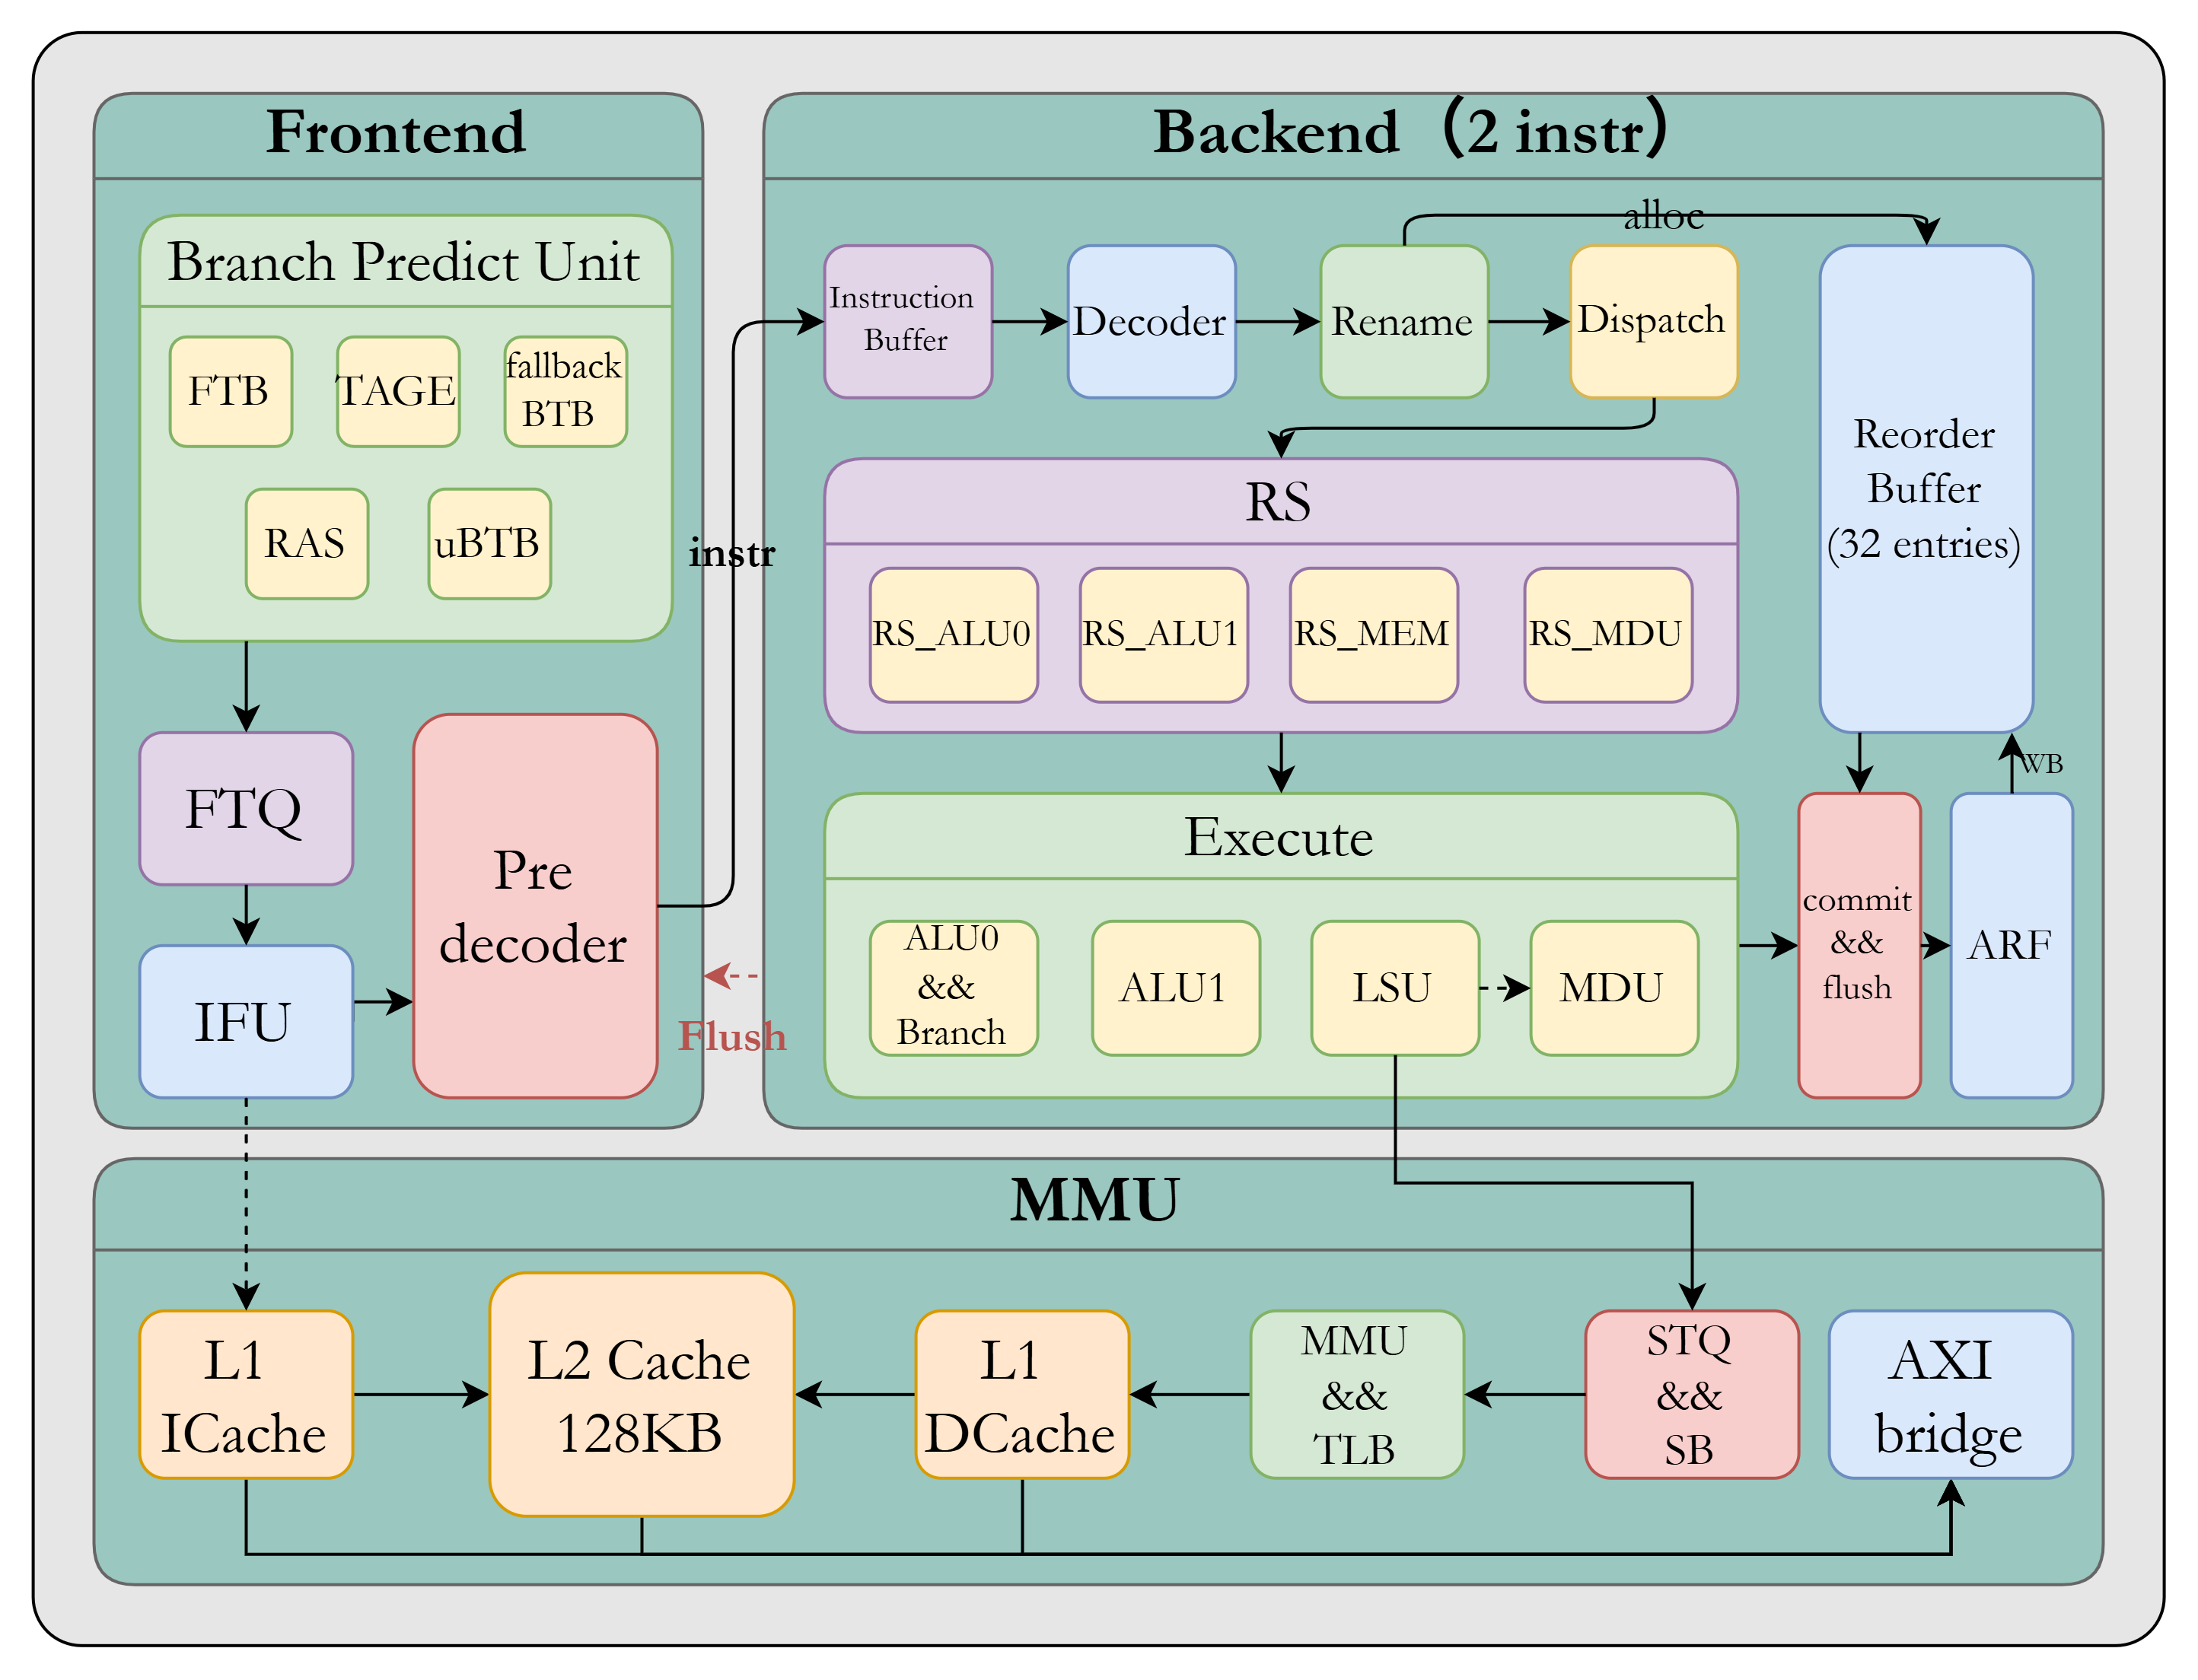
\includegraphics[width=0.95\textwidth]{figure/mycpu_arch.png}
  \caption{CPU 设计架构图}
  \label{fig:cpuarch}
\end{figure}

意味核采用前后端解耦的乱序结构。前端由分支预测器、FTQ、IFU、ICache 和 IB 组成，以最多 4 条指令的基本块推进；后端由译码、重命名、分发、异构保留站、三路 ALU、LSU、MDU、ROB 与提交控制组成。ROB 编号直接作为重命名标签，结果保存在 ROB 中，已提交的 ARF 是全局恢复后的权威状态，不设置独立 PRF 与 freelist。

处理器以 2 宽作为稳定基线：常规路径每拍处理两条指令；当 IB 中第三条指令满足资源与类型约束时，可机会式进入第三译码、重命名和分发通路，三条均为 ALU 类时可使用三路整数执行单元。提交级通常退休 2 条指令，在队首两条正常提交且下一对简单指令均已完成、无例外和串行副作用时，可启用受限四退休快路径。

指令执行过程如下：
\begin{enumerate}
  \item \textbf{预测与取指}：BPU 生成最多 4 条指令的预测块，FTQ 保存预测元数据，IFU 经 MMU 与 ICache 取回指令并写入 IB；
  \item \textbf{译码与重命名}：生成操作类型、立即数、特权和例外信息，查询 RAT/ARF/ROB 获得源操作数，以 ROB 编号建立寄存器依赖；
  \item \textbf{分发与发射}：按 ALU、MEM、MDU 三类路由到异构保留站，在操作数和功能单元就绪后发射；
  \item \textbf{执行与写回}：ALU、LSU 和 MDU 完成运算，将结果、分支结果或例外信息写回 ROB；
  \item \textbf{按序提交}：提交级更新 ARF、CSR、TLB、LLBit 与 Store Buffer，并统一处理分支误预测、例外、\texttt{ertn} 和缓存维护引起的重取。
\end{enumerate}

\begin{table}[H]
\centering
\caption{主要结构容量}
\label{tab:capacity}
\small
\begin{tabularx}{\textwidth}{>{\raggedright\arraybackslash}p{3.3cm}X}
\toprule
结构 & 规格 \\
\midrule
取指与后端宽度 & 每块最多 4 条取指；2 宽基线；机会式三宽译码、重命名与分发；受限四退休 \\
ROB & 32 项，奇偶双体组织 \\
IB / FTQ & 16 项 / 16 项 \\
保留站 & RS\_ALU $3\times5$ 项；RS\_MEM 8 项；RS\_MDU 2 项 \\
STQ / Store Buffer & 16 项 / 8 项 \\
L1 Cache & ICache、DCache 各 16\,KiB，4 路$\times$128 组$\times$32\,B，VIPT \\
L2 Cache & 128\,KiB，2 路$\times$2048 组$\times$32\,B，写回式 \\
TLB & 主 TLB 32 项、双查询口；I/D 微 TLB 各 8 项 \\
BPU & uBTB 32 项；fallback BTB 128 项；FTB $4\times2048$；TAGE 8K$+4\times2$K；局部预测器；RAS 32 双栈 \\
\bottomrule
\end{tabularx}
\end{table}

\subsubsection{指令实现}

处理器实现表~\ref{tab:inst} 所列 LA32R 整数与特权指令子集。\texttt{preld} 被识别为合法指令并以无执行副作用的方式退休；\texttt{ibar}/\texttt{dbar} 在提交级等待 Store Buffer 排空后触发重取，从而保证屏障之前的访存已经对系统可见。当前实现不包含浮点与向量执行单元。

\begin{table}[H]
\centering
\caption{指令实现}
\label{tab:inst}
\scriptsize
\begin{tabularx}{\textwidth}{>{\raggedright\arraybackslash}p{2.7cm}X}
\toprule
指令类型 & 指令名称 \\
\midrule
算术与逻辑 & \texttt{add.w}, \texttt{sub.w}, \texttt{addi.w}, \texttt{slt}, \texttt{sltu}, \texttt{slti}, \texttt{sltui}, \texttt{lu12i.w}, \texttt{pcaddu12i}, \texttt{pcaddi}, \texttt{and}, \texttt{or}, \texttt{nor}, \texttt{xor}, \texttt{andn}, \texttt{orn}, \texttt{andi}, \texttt{ori}, \texttt{xori} \\
移位 & \texttt{sll.w}, \texttt{srl.w}, \texttt{sra.w}, \texttt{slli.w}, \texttt{srli.w}, \texttt{srai.w} \\
乘除 & \texttt{mul.w}, \texttt{mulh.w}, \texttt{mulh.wu}, \texttt{div.w}, \texttt{div.wu}, \texttt{mod.w}, \texttt{mod.wu} \\
分支跳转 & \texttt{beq}, \texttt{bne}, \texttt{blt}, \texttt{bltu}, \texttt{bge}, \texttt{bgeu}, \texttt{b}, \texttt{bl}, \texttt{jirl} \\
普通访存 & \texttt{ld.b}, \texttt{ld.bu}, \texttt{ld.h}, \texttt{ld.hu}, \texttt{ld.w}, \texttt{st.b}, \texttt{st.h}, \texttt{st.w} \\
原子访存 & \texttt{ll.w}, \texttt{sc.w} \\
屏障与预取 & \texttt{ibar}, \texttt{dbar}, \texttt{preld} \\
特权与 TLB & \texttt{csrrd}, \texttt{csrwr}, \texttt{csrxchg}, \texttt{tlbsrch}, \texttt{tlbrd}, \texttt{tlbwr}, \texttt{tlbfill}, \texttt{invtlb}, \texttt{cacop}, \texttt{ertn}, \texttt{idle} \\
系统与计时器 & \texttt{syscall}, \texttt{break}, \texttt{rdcntid}, \texttt{rdcntvl.w}, \texttt{rdcntvh.w}, \texttt{cpucfg} \\
\bottomrule
\end{tabularx}
\end{table}

\subsubsection{CSR 实现}

CSR 模块保存处理器模式、例外、中断、计时器、TLB 和直接映射窗口状态。未实现编号的 CSR 读返回 0、写忽略；TICLR、SAVE0--3、TID 等低风险寄存器采用快速写路径，其他会改变执行环境的 CSR 写在提交级串行完成。

\begin{table}[H]
\centering
\caption{主要 CSR}
\label{tab:csr}
\scriptsize
\begin{tabularx}{\textwidth}{cXlcXl}
\toprule
地址 & 含义 & 名称 & 地址 & 含义 & 名称 \\
\midrule
0x0 & 当前模式信息 & CRMD & 0x30--33 & 数据保存 & SAVE0--3 \\
0x1 & 例外前模式信息 & PRMD & 0x40 & 定时器编号 & TID \\
0x2 & 扩展组件使能 & EUEN & 0x41 & 定时器配置 & TCFG \\
0x4 & 例外配置 & ECFG & 0x42 & 定时器值 & TVAL \\
0x5 & 例外状态 & ESTAT & 0x44 & 定时中断清除 & TICLR \\
0x6 & 例外返回地址 & ERA & 0x60 & LLBit 控制 & LLBCTL \\
0x7 & 出错虚地址 & BADV & 0x88 & TLB 重填入口 & TLBRENTRY \\
0xC & 例外入口地址 & EENTRY & 0x180--181 & 直接映射窗口 & DMW0--1 \\
0x10 & TLB 索引 & TLBIDX & 0x18 & 地址空间编号 & ASID \\
0x11 & TLB 表项高位 & TLBEHI & 0x19--1B & 页目录基址 & PGDL/H/D \\
0x12--13 & TLB 表项低位 & TLBELO0/1 & 0x20 & 处理器编号 & CPUID \\
\bottomrule
\end{tabularx}
\end{table}

\subsubsection{例外与中断}

例外信息随指令在流水线中传递，最终在提交级按优先级编码并更新 CSR，以保证精确例外。8 路外部硬中断接入 ESTAT.IS[9:2]，定时器中断接入 ESTAT.IS[11]。\texttt{idle} 退休后停止取指，直至可响应中断到来。

\begin{table}[H]
\centering
\caption{例外与中断类型}
\label{tab:excp}
\small
\begin{tabular}{cccc}
\toprule
Ecode & Esubcode & 代号 & 类型 \\
\midrule
0x0 & 0 & INT & 中断 \\
0x1 & 0 & PIL & Load 页无效 \\
0x2 & 0 & PIS & Store 页无效 \\
0x3 & 0 & PIF & 取指页无效 \\
0x4 & 0 & PME & 页修改 \\
0x7 & 0 & PPI & 页特权等级不合规 \\
0x8 & 0 & ADEF & 取指地址错误 \\
0x8 & 1 & ADEM & 访存地址错误 \\
0x9 & 0 & ALE & 地址非对齐 \\
0xB & 0 & SYS & 系统调用 \\
0xC & 0 & BRK & 断点 \\
0xD & 0 & INE & 指令不存在 \\
0xE & 0 & IPE & 指令特权等级错误 \\
0x3F & 0 & TLBR & TLB 重填 \\
\bottomrule
\end{tabular}
\end{table}

\subsubsection{地址翻译模式}

CRMD.DA$=1$、PG$=0$ 时采用直接地址；DA$=0$、PG$=1$ 时先匹配 DMW0/DMW1，未命中窗口则查询 TLB。TLB 表项同时给出物理页号、页大小、有效位、脏位、特权等级和存储访问类型，相关例外随取指或访存指令进入 ROB，并在提交级处理。

\subsection{前端设计}

\begin{figure}[H]
  \centering
  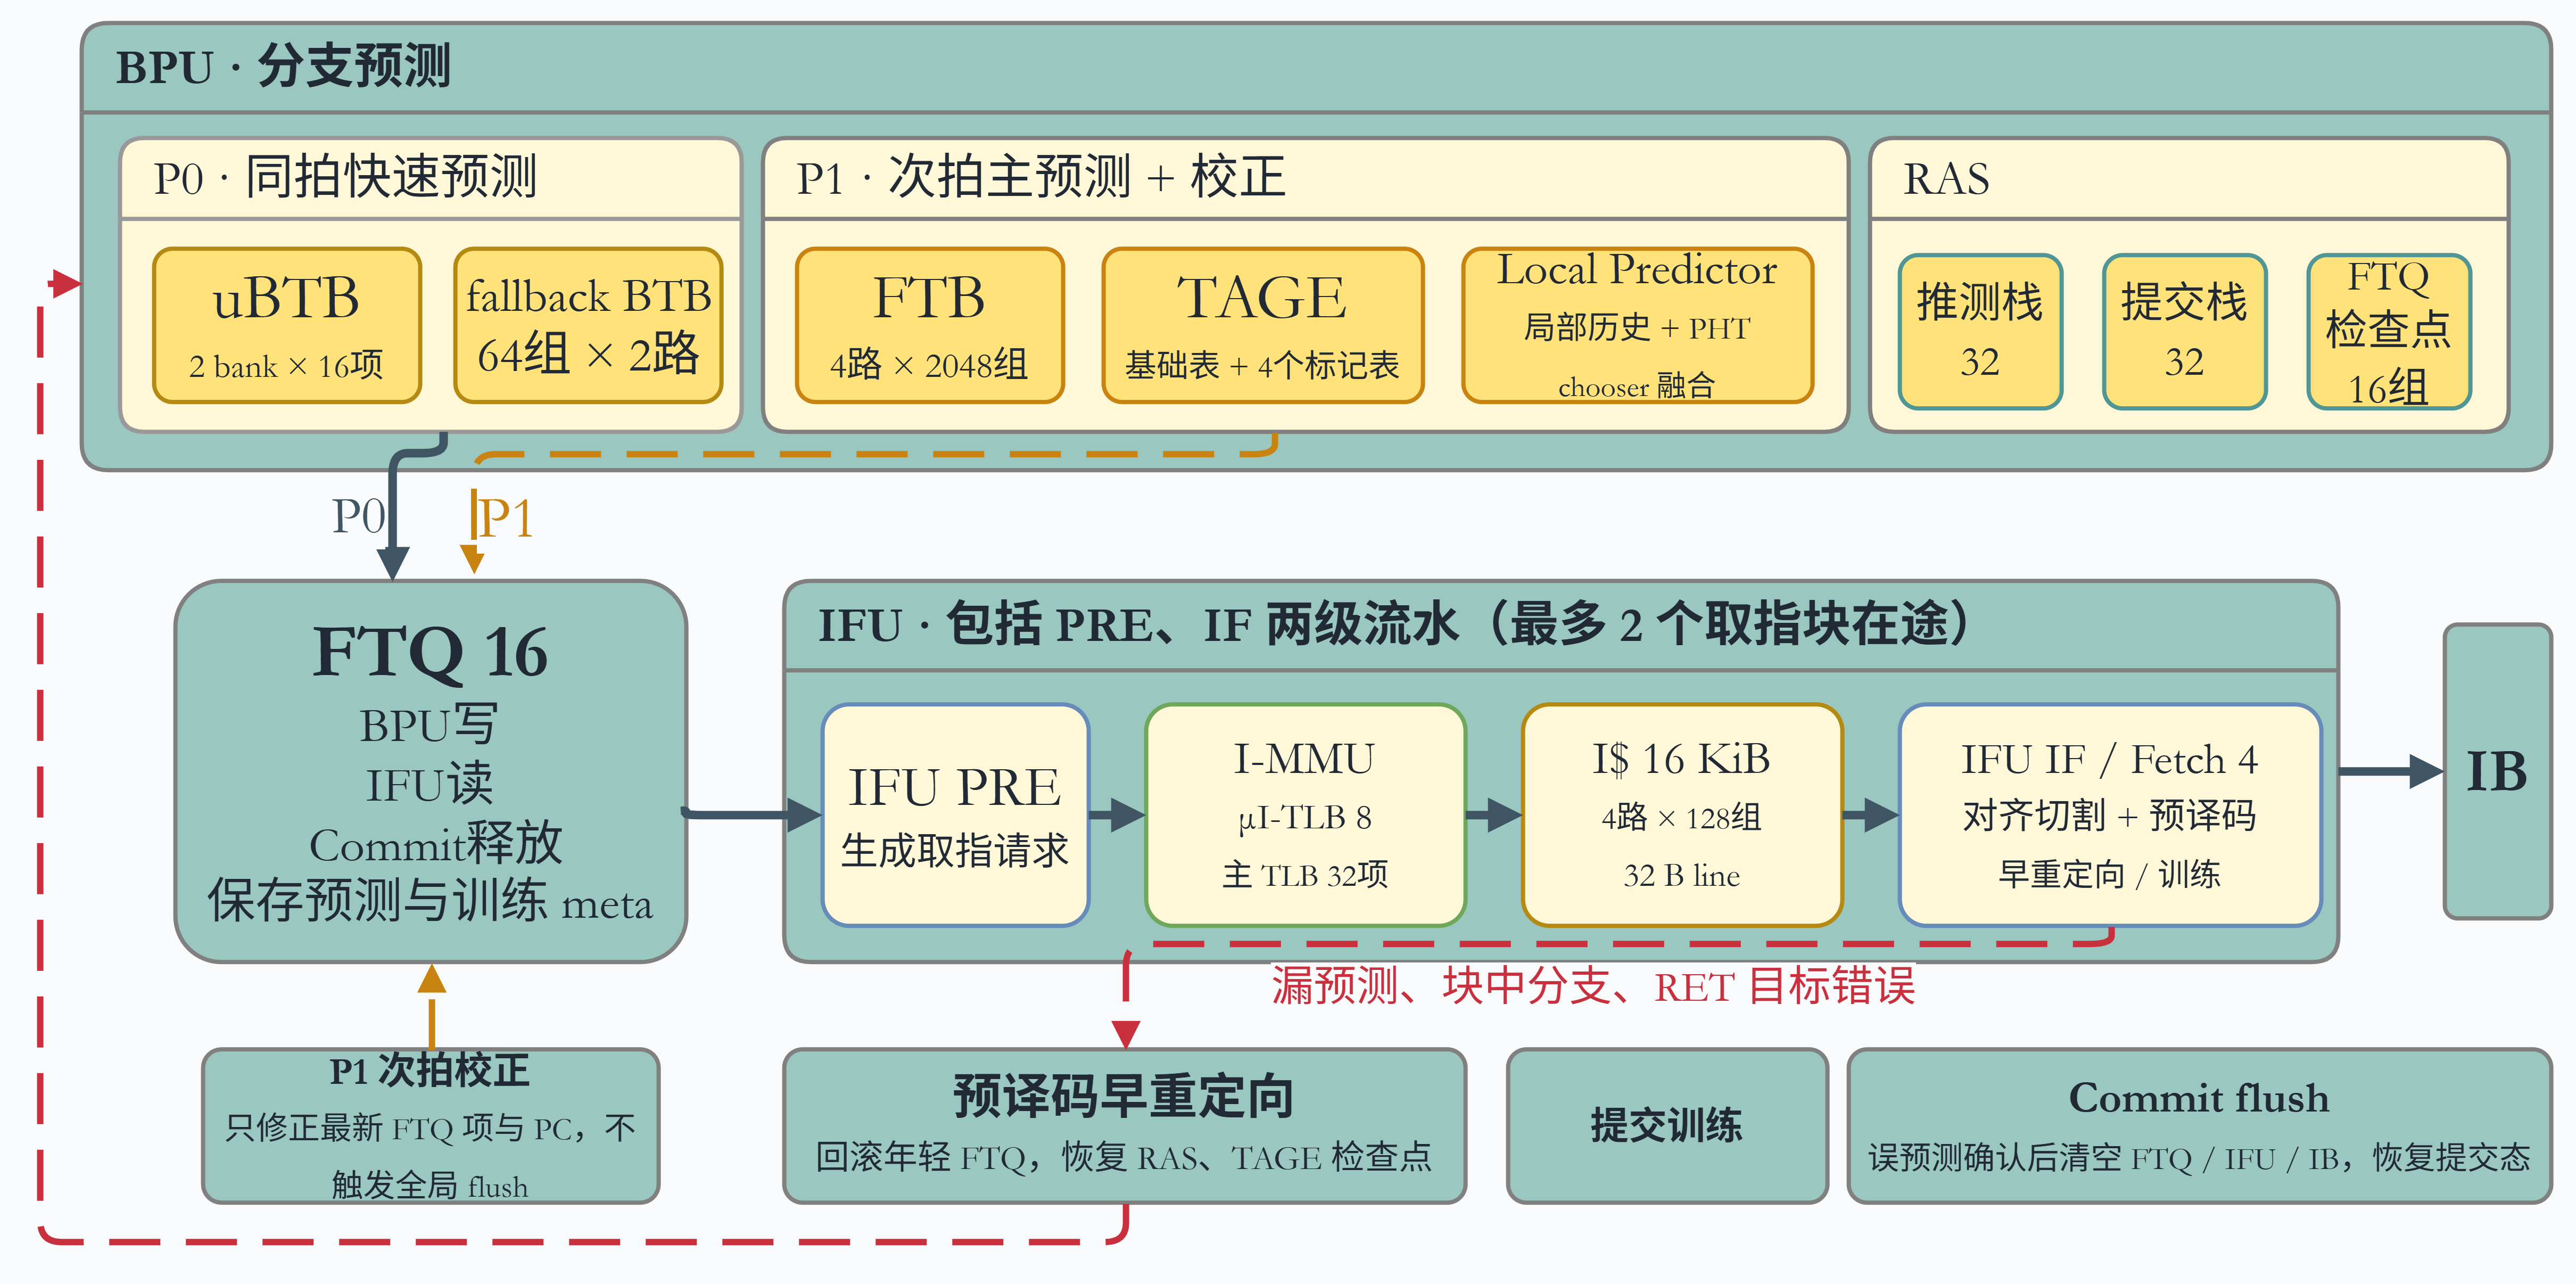
\includegraphics[width=0.95\textwidth]{figure/frontend.png}
  \caption{前端架构图}
  \label{fig:frontend}
\end{figure}

前端采用基本块取指结构，主要包含分支预测器（BPU）、取指目标队列（FTQ）、取指单元（IFU）、一级指令缓存（ICache）和指令缓冲（IB）。BPU 每拍针对一个起始 PC 产生一个预测块，块内最多包含 4 条指令，并在 4\,KB 页边界处截断，避免一次预测跨越两个地址翻译页。

\subsubsection{分支预测器}

分支预测器采用 P0/P1 两级响应。P0 使用快速结构当拍给出基线预测，P1 在下一拍返回容量更大的主预测结果；若两级结果不一致，则修正 FTQ 中对应条目并重定向前端。

\begin{itemize}
  \item \textbf{uBTB}：两银行、每银行 16 项，共 32 个物理表项；每次查询一个 16 路全相联银行，提供 P0 快速目标；
  \item \textbf{fallback BTB}：两路、每路 64 组，共 128 项，在 uBTB 未命中时提供快速后备目标；
  \item \textbf{FTB}：4 路$\times$2048 组，共 8192 项，保存基本块内分支位置、类型、目标和顺序下落地址；
  \item \textbf{TAGE}：8192 项基础计数表与 4 张各 2048 项、12 位标签的历史表，全局历史长度为 4/10/24/64；
  \item \textbf{局部预测器}：2048 项、每项 12 位的局部历史表，配合 4096 项两位计数 PHT 与选择器，补充规律性局部分支；
  \item \textbf{RAS}：32 项推测栈和 32 项提交栈组成双栈，在函数调用/返回预测与提交恢复之间隔离投机状态。
\end{itemize}

各预测结构按其职责分别维护推测态与提交态。TAGE 和局部方向预测器以提交结果更新计数与已提交历史，同时在取指路径维护可恢复的推测历史；BTB/FTB 除提交更新外，还可由 IFU 预译码对直接跳转进行早填充。RAS 在 P1 阶段执行推测 push/pop，并通过 checkpoint 在冲刷时恢复，提交栈用于保持架构确认状态。

\subsubsection{取指目标队列 FTQ}

FTQ 深度为 16，使用 BPU 写指针、IFU 读指针和提交释放指针管理环形队列。每项保存预测块起始 PC、顺序下落地址、目标、分支类型和各级预测器元数据。P0 结果先入队，P1 可以就地修正上一拍条目；提交级按程序顺序释放 FTQ 项并回送训练结果。

\subsubsection{IFU 与取指流水}

IFU 从 FTQ 读取预测块，经 MMU 完成取指地址翻译后访问 ICache。取指流水主要包括：
\begin{itemize}
  \item \textbf{PRE}：接收 FTQ 条目，进行页边界检查和地址翻译，满足条件时向 ICache 发起整行读取；
  \item \textbf{IF}：等待 Cache 行返回，按预测块起止位置切分至多 4 条指令并写入 IB；
  \item \textbf{预译码重定向}：检查无需寄存器操作数即可确定的直接跳转，发现漏预测时提前刷新前端；
  \item \textbf{冲刷协同}：提交级全局冲刷时清空流水寄存器；若已有 ICache 事务在途，则丢弃其迟到返回。
\end{itemize}

执行 \texttt{cacop} 等指令维护操作时，IFU 与 ICache 串行完成维护并清理前端状态，避免自修改代码路径继续使用旧指令。

\subsection{指令缓冲（IB）模块设计}

IB 位于取指前端与后端之间，用于吸收 ICache miss、分支修正和后端停顿造成的带宽波动。队列深度为 16，每拍最多接收 4 条取指结果，并向后端提供 3 个弹出端口；前两条构成稳定的 2 宽基线，第三条只在译码、重命名、ROB 与目标保留站均允许时机会式使用。

每个 IB 表项保存有效位、PC、指令码、分支预测信息、所属 FTQ 编号以及取指阶段产生的地址和例外信息。入队端根据实际有效指令数紧凑写入连续空位，出队端在后端确认接收后移动读指针，因而 1--4 条可变宽入队不会留下气泡。

后端停顿时 IB 保持队头内容稳定；提交级误预测、例外、\texttt{ertn} 或缓存维护重取会清空全部投机表项。该设计使 BPU/IFU 可以继续在短时后端阻塞期间预取，同时又能在统一恢复点快速丢弃错误路径。

\subsection{后端设计}

\begin{figure}[H]
  \centering
  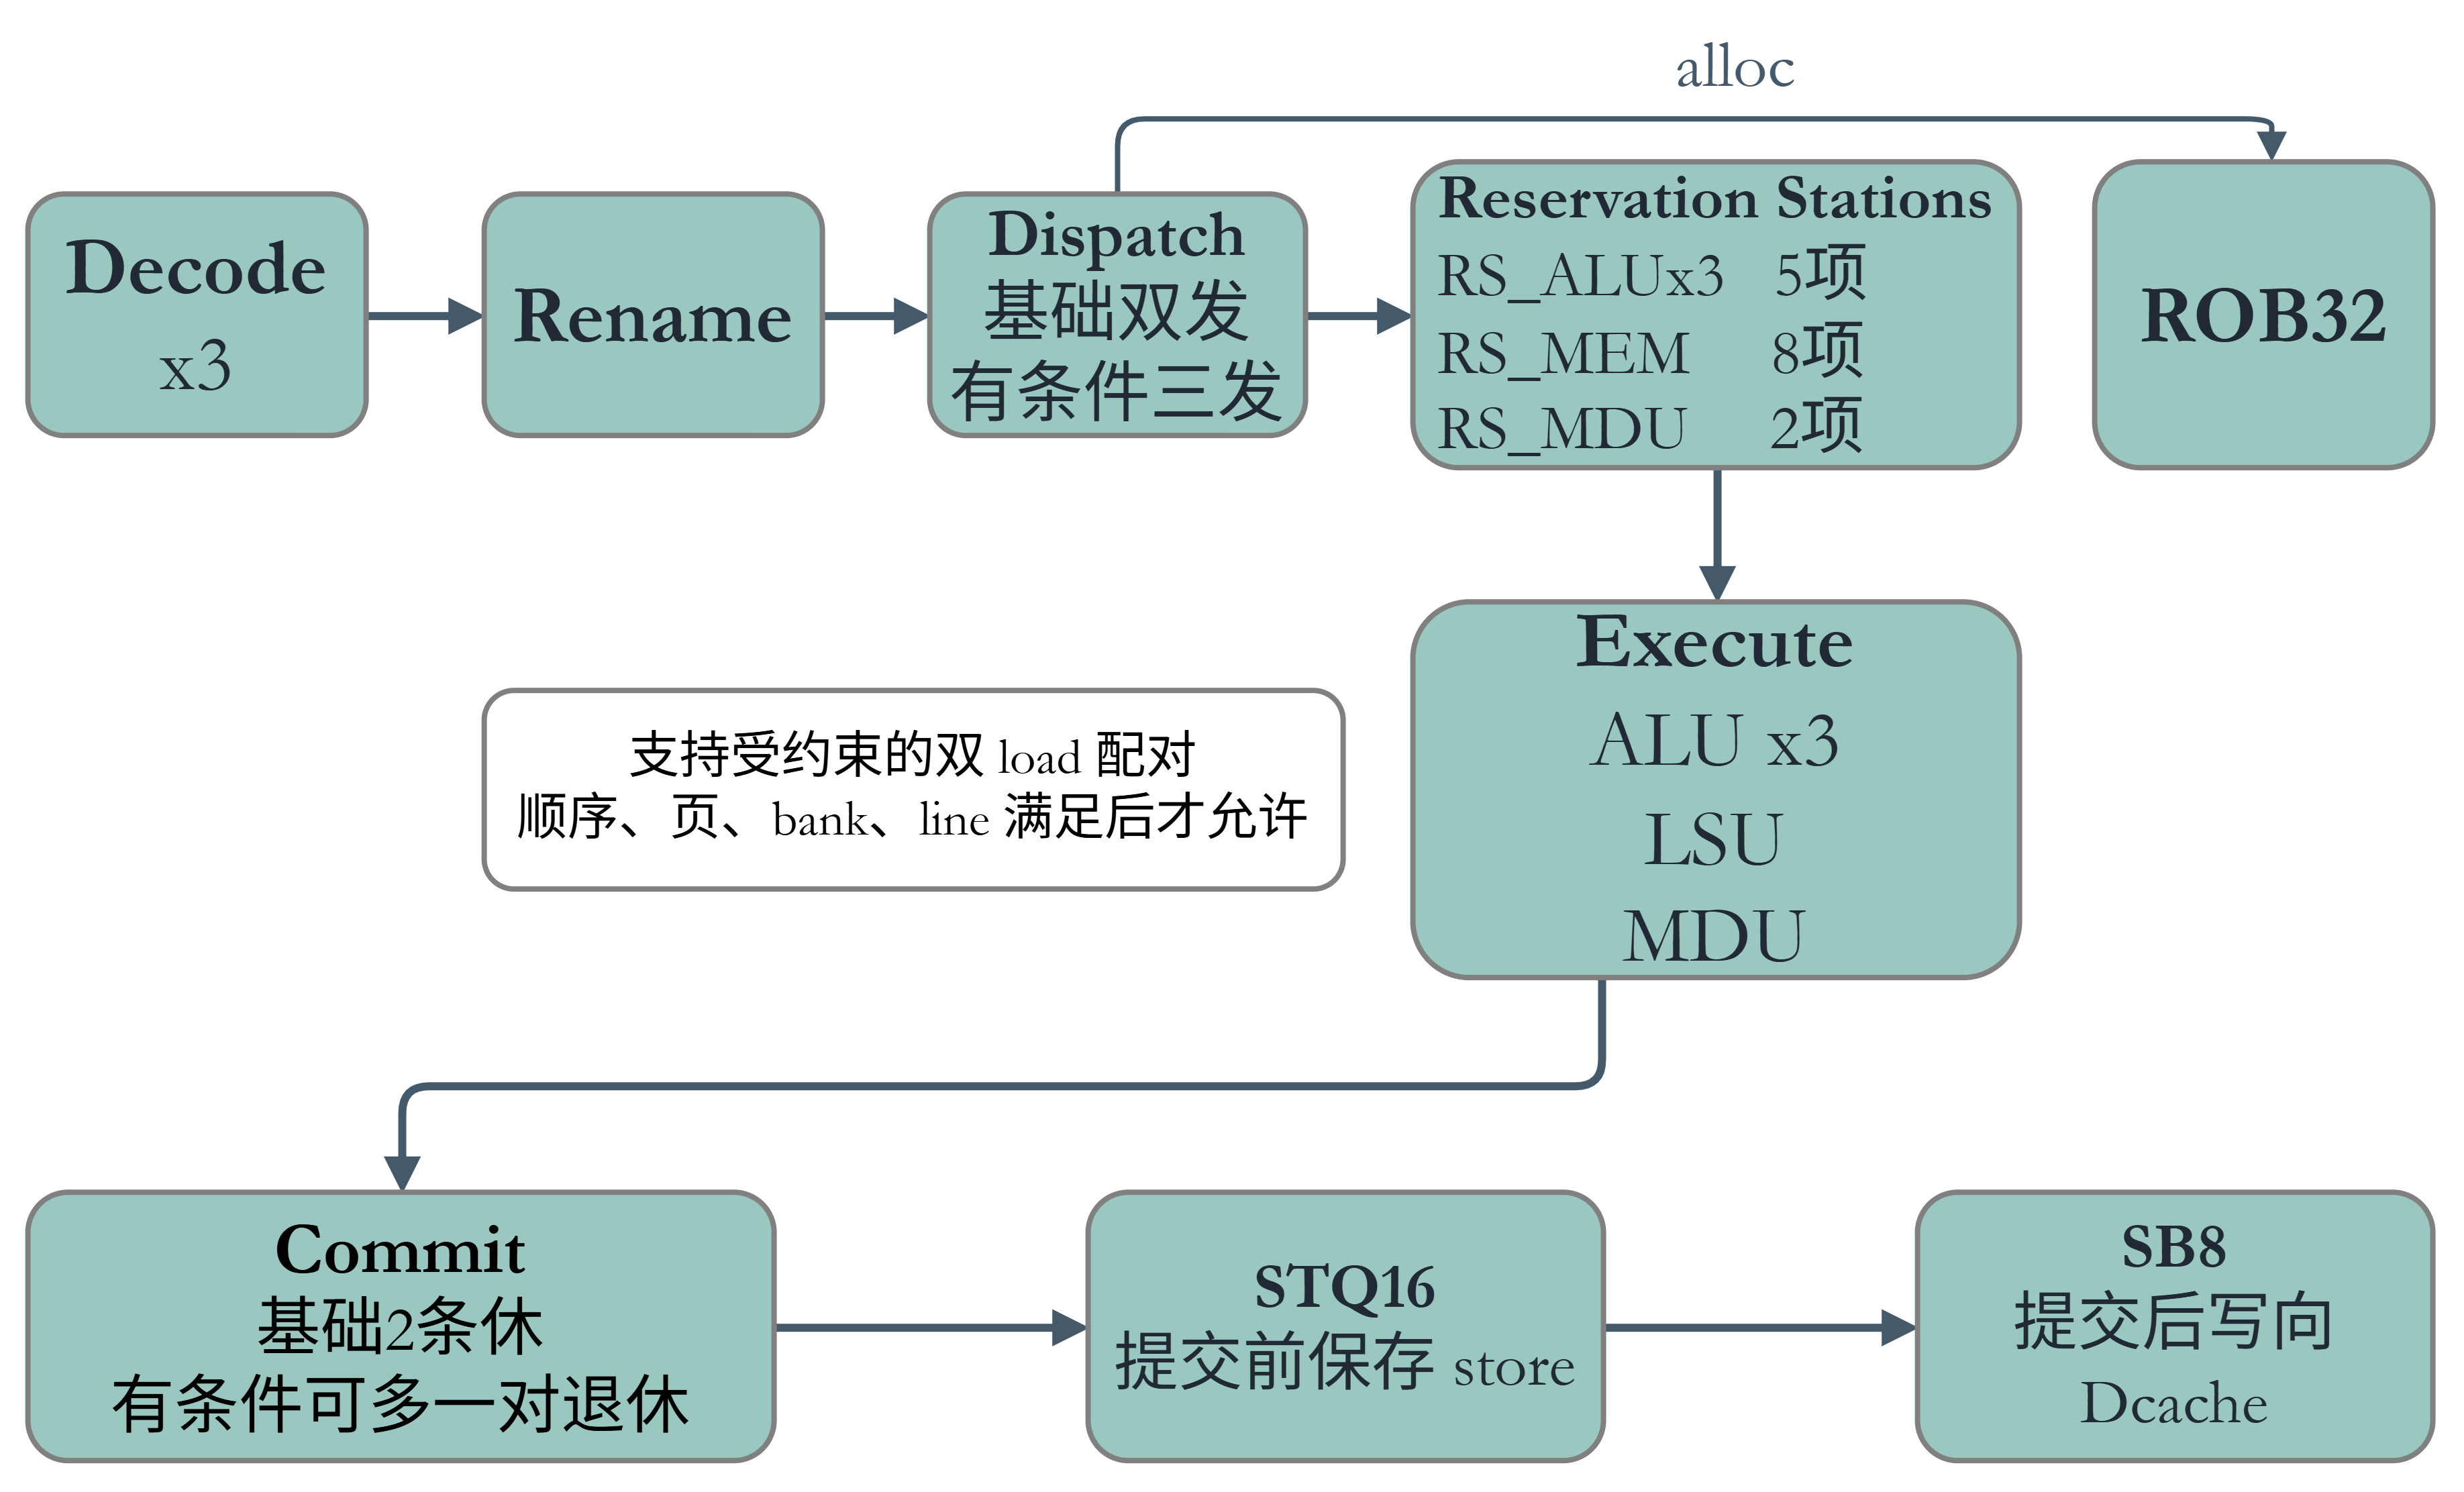
\includegraphics[width=0.95\textwidth]{figure/backend.png}
  \caption{后端架构图}
  \label{fig:backend}
\end{figure}

后端采用“2 宽基线、机会式三宽”的乱序组织，逻辑阶段为译码、重命名、分发、保留站发射、执行写回和按序提交。寄存器依赖以 ROB 编号表示，运算结果保存在 ROB；ARF 只在提交时更新，是例外或误预测恢复后的架构状态。

\subsubsection{译码与重命名}

IB 的前两条指令进入常规译码路径；第三条在资源满足时通过机会式通路继续推进。译码器生成 FU 类型、独热操作码、立即数、源/目的寄存器、访存宽度、分支类型、CSR/TLB/Cache 维护标记和例外向量。

RAT 为 32 项逻辑寄存器映射表，记录 busy 状态和最新生产者的 ROB 编号。重命名级从 RAT、ARF 和已完成 ROB 项中选择源操作数，并处理同拍指令之间的 RAW/WAW 关系。写寄存器指令更新 RAT；提交时仅在退休项仍为最新生产者时清除对应 busy。

\subsubsection{分发与保留站}

分发单元补齐可从 ROB 旁路得到的源操作数，并按类型送入异构保留站：
\begin{itemize}
  \item \textbf{RS\_ALU0/1/2}：三组、每组 5 项，从就绪项中选择指令；三条均为 ALU 类且三个执行通路可接收时可同拍三发；
  \item \textbf{RS\_MEM}：8 项。完整 SoC 模式仅允许队首访存发射，以保持 Linux 和 MMIO 顺序；性能模式可在连续且已确认 cached 的窗口内扫描最多 4 项，并启用成对 Load 优化；
  \item \textbf{RS\_MDU}：2 项 FIFO，服务乘除、CSR 读、计时器、\texttt{cpucfg} 和 TLB 维护准备操作。
\end{itemize}

unknown、TLB、uncached、MMIO 或顺序敏感访存会终止年轻访存旁路。CSR 写、TLB 修改、屏障和例外等架构副作用不在发射级生效，而在提交级串行执行。

\subsubsection{执行单元}

\begin{itemize}
  \item \textbf{ALU0/1/2}：完成整数算术、逻辑、移位、比较和分支目标计算，并将结果或分支判定写回 ROB；
  \item \textbf{LSU}：由 AGU 与 DCache 访问级组成。AGU 计算虚地址、调用 MMU 并检查对齐和页例外；后级执行 STQ/SB 前递、Cache/uncached 访问和 miss 管理；
  \item \textbf{MDU}：乘法使用寄存后的 DSP 乘积，启动后一拍完成；除法先用 CLZ 对齐，再按有效位数迭代，延迟随操作数变化。
\end{itemize}

尚未提交的 Store 保存在 16 项 STQ 中，为年轻 Load 提供顺序检查与安全前递；Store 退休后转入 8 项 Store Buffer。Store Buffer 保存已提交写操作，因此全局冲刷不会清空其内容。

\subsubsection{ROB 与提交}

ROB 共 32 项，采用奇偶双体环形组织。表项保存 PC、目的寄存器、执行结果、访存信息、预测元数据、CSR/TLB 操作和例外向量。功能单元写回后置位 complete，提交级始终从队首按程序顺序检查。

正常情况下每拍最多退休两条指令。当前两条可正常提交，且后续一对均为已完成、无例外、无分支和无串行副作用的简单指令时，可同时退休下一对，峰值为 4 条。\texttt{ll}/\texttt{sc}、CSR/TLB、屏障、\texttt{cacop}、例外和 \texttt{ertn} 会限制提交宽度。

\subsubsection{统一冲刷与精确例外}

误预测、例外、\texttt{ertn} 和需要重取的特权操作均由提交级产生全局冲刷。冲刷清空前端、RAT、ROB 和各保留站的投机状态，以已提交 ARF、CSR 与 Store Buffer 为恢复基础，再从正确 PC 重新取指。该方案没有复杂的选择性历史回滚，保证了精确例外与已提交访存不丢失。

\subsection{AXI Line Bridge}

CPU 顶层提供 32 位地址、32 位数据、4 位 ID 的 AXI 主接口，包含 AR/R/AW/W/B 五通道，并保留 SoC 互连所需的写数据 ID。\texttt{axi\_line\_bridge} 位于 L2 与该接口之间，将 32\,B Cache 行转换为 8 拍、每拍 32 位的 INCR burst。

\begin{itemize}
  \item \textbf{行读取}：\texttt{ARLEN}=7。指令和数据读取分别使用 ID 0/1，最多允许两路读取在途，R 通道按 ID 分流；
  \item \textbf{行写回}：\texttt{AWLEN}=7，上游分段送入整行数据，桥接器缓存并产生 8 拍写突发，最多允许两笔写响应在途；
  \item \textbf{Uncached 访问}：根据字节、半字或字访问设置 \texttt{ARSIZE}/\texttt{AWSIZE} 和写掩码，设备写等待 B 响应后才完成；
  \item \textbf{顺序约束}：存在未完成写事务时限制新的读请求，避免脏行写回与同地址 refill 发生可见次序倒置。
\end{itemize}

当前桥接器接收但不解释 \texttt{RRESP} 与 \texttt{BRESP}，因此不会把 AXI slave error 转换为处理器总线例外。这是现有接口的功能边界。CPU/uncore 跨时钟域由 SoC 中的 AXI Clock Converter 完成，不在核内桥接器中处理。

\subsection{Cache 与访存层次}

\begin{figure}[H]
  \centering
  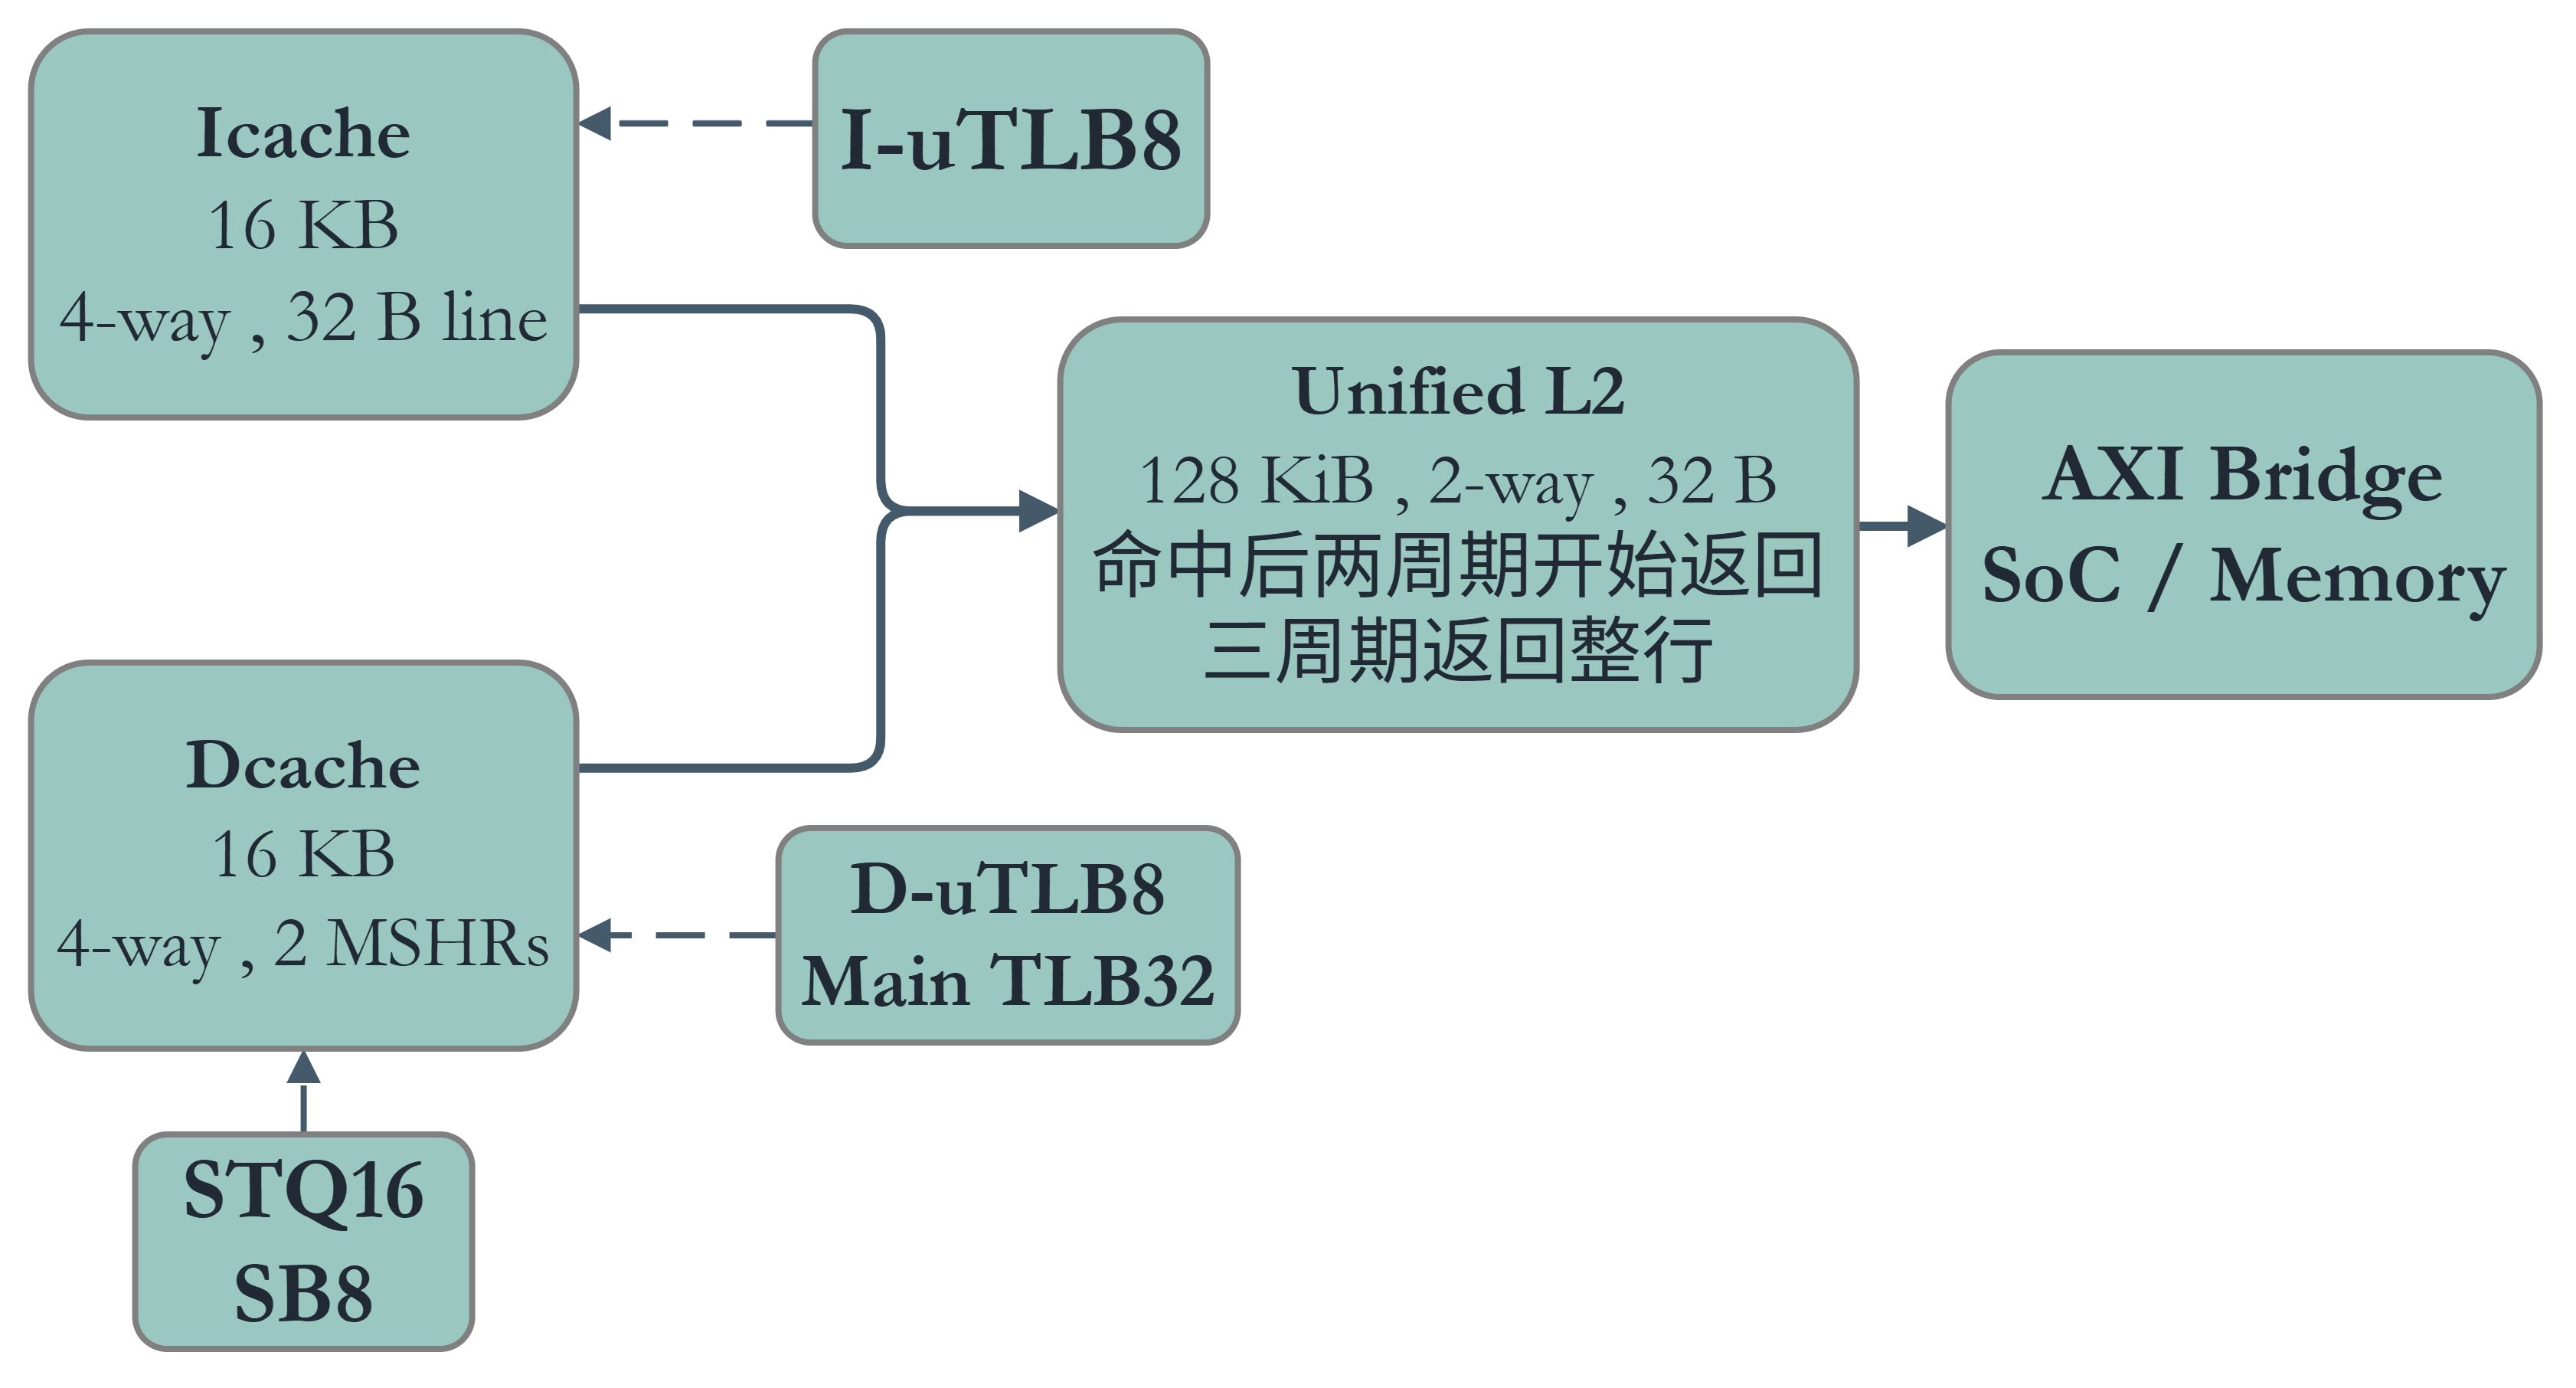
\includegraphics[width=0.95\textwidth]{figure/memory.png}
  \caption{访存架构图}
  \label{fig:memory}
\end{figure}

意味核采用 ICache/DCache、统一 L2 Cache 和 AXI 行桥的三级访问路径，并以 STQ 与 Store Buffer 分离投机 Store 和已提交 Store。

\subsubsection{一级指令缓存}

ICache 容量为 16\,KB，组织为 4 路$\times$128 组$\times$32\,B，采用 VIPT 查询。命中时向 IFU 返回完整 Cache 行；缺失时通过单一 miss 状态机向 L2 请求 refill。\texttt{cacop} 维护请求在当前事务完成后串行执行，在途返回若已因前端冲刷失效则不再写入取指流水。

\subsubsection{一级数据缓存}

DCache 同样为 16\,KiB、4 路$\times$128 组$\times$32\,B、VIPT，面向 LSU 的 Load/Store。两个 MSHR 支持 hit-under-miss，并可合并同一 Cache 行上的后续 Load。命中路径结合 STQ/SB 前递，缺失路径访问 L2；脏行替换采用写回策略。

\subsubsection{统一二级缓存}

L2 容量为 128\,KB，2 路$\times$2048 组$\times$32\,B，供 ICache 与 DCache 共享。L2 具有 I/D 独立下游读端口、4 项 victim buffer 和写回控制，可在 DCache refill 时尽早向上游返回所需数据。保守的 ICache next-line 与 DCache stream 预取在不破坏需求访问优先级的前提下减少连续访问 miss。

\subsubsection{STQ 与 Store Buffer}

\begin{itemize}
  \item \textbf{STQ（16 项）}：保存未提交 Store，按 ROB 顺序提供 Load 相关性检查与数据前递；错误路径冲刷时相应投机项被清除；
  \item \textbf{Store Buffer（8 项）}：保存已提交 Store，可合并同一 Cache 行或相邻写掩码，再写入 DCache/L2；其内容在全局冲刷后继续排空。
\end{itemize}

LSU 优先检查 STQ 与 Store Buffer 前递，再访问 DCache。已确认的数据旁路可以提前完成对应 ROB 项，从而降低访存密集程序的提交阻塞。

\subsection{地址翻译设计}

\subsubsection{MMU 模块}

MMU 为 IFU 与 LSU 提供独立翻译通路，根据 CRMD、DMW0/1、ASID 和访问类型在直接地址、直接映射窗口与 TLB 页映射之间选择。返回结果包括物理地址、MAT（cached/uncached）、页权限和例外信息。

\subsubsection{主 TLB 与微 TLB}

主 TLB 为 32 项全相联结构，具有指令、数据两个查询口，支持 4\,KB 与 4\,MB 页，并提供 \texttt{tlbsrch}、\texttt{tlbrd}、\texttt{tlbwr}、\texttt{tlbfill} 和 \texttt{invtlb} 维护端口。

取指和访存通路前各设置 8 项微 TLB，只缓存常用 4\,KB 翻译。微 TLB 命中可在当前拍完成；未命中时查询主 TLB，结果由管理器登记并在下一拍交付请求方。大页请求直接使用主 TLB 结果。

TLBR、PIL/PIS/PIF、PPI、PME 与地址类例外随对应指令进入 ROB，提交级更新 BADV、ESTAT 等 CSR，并重定向到 EENTRY 或 TLBRENTRY。TLB 维护和 CSR 地址空间切换均在提交级串行完成，防止年轻指令观察到部分更新状态。

\subsection{SoC 设计}
在 SOC 顶层实例化了我们的 CPU ，向 SoC 提供单路 32 位 AXI 主接口和 8 路外部中断输入。

\begin{figure}[H]
  \centering
  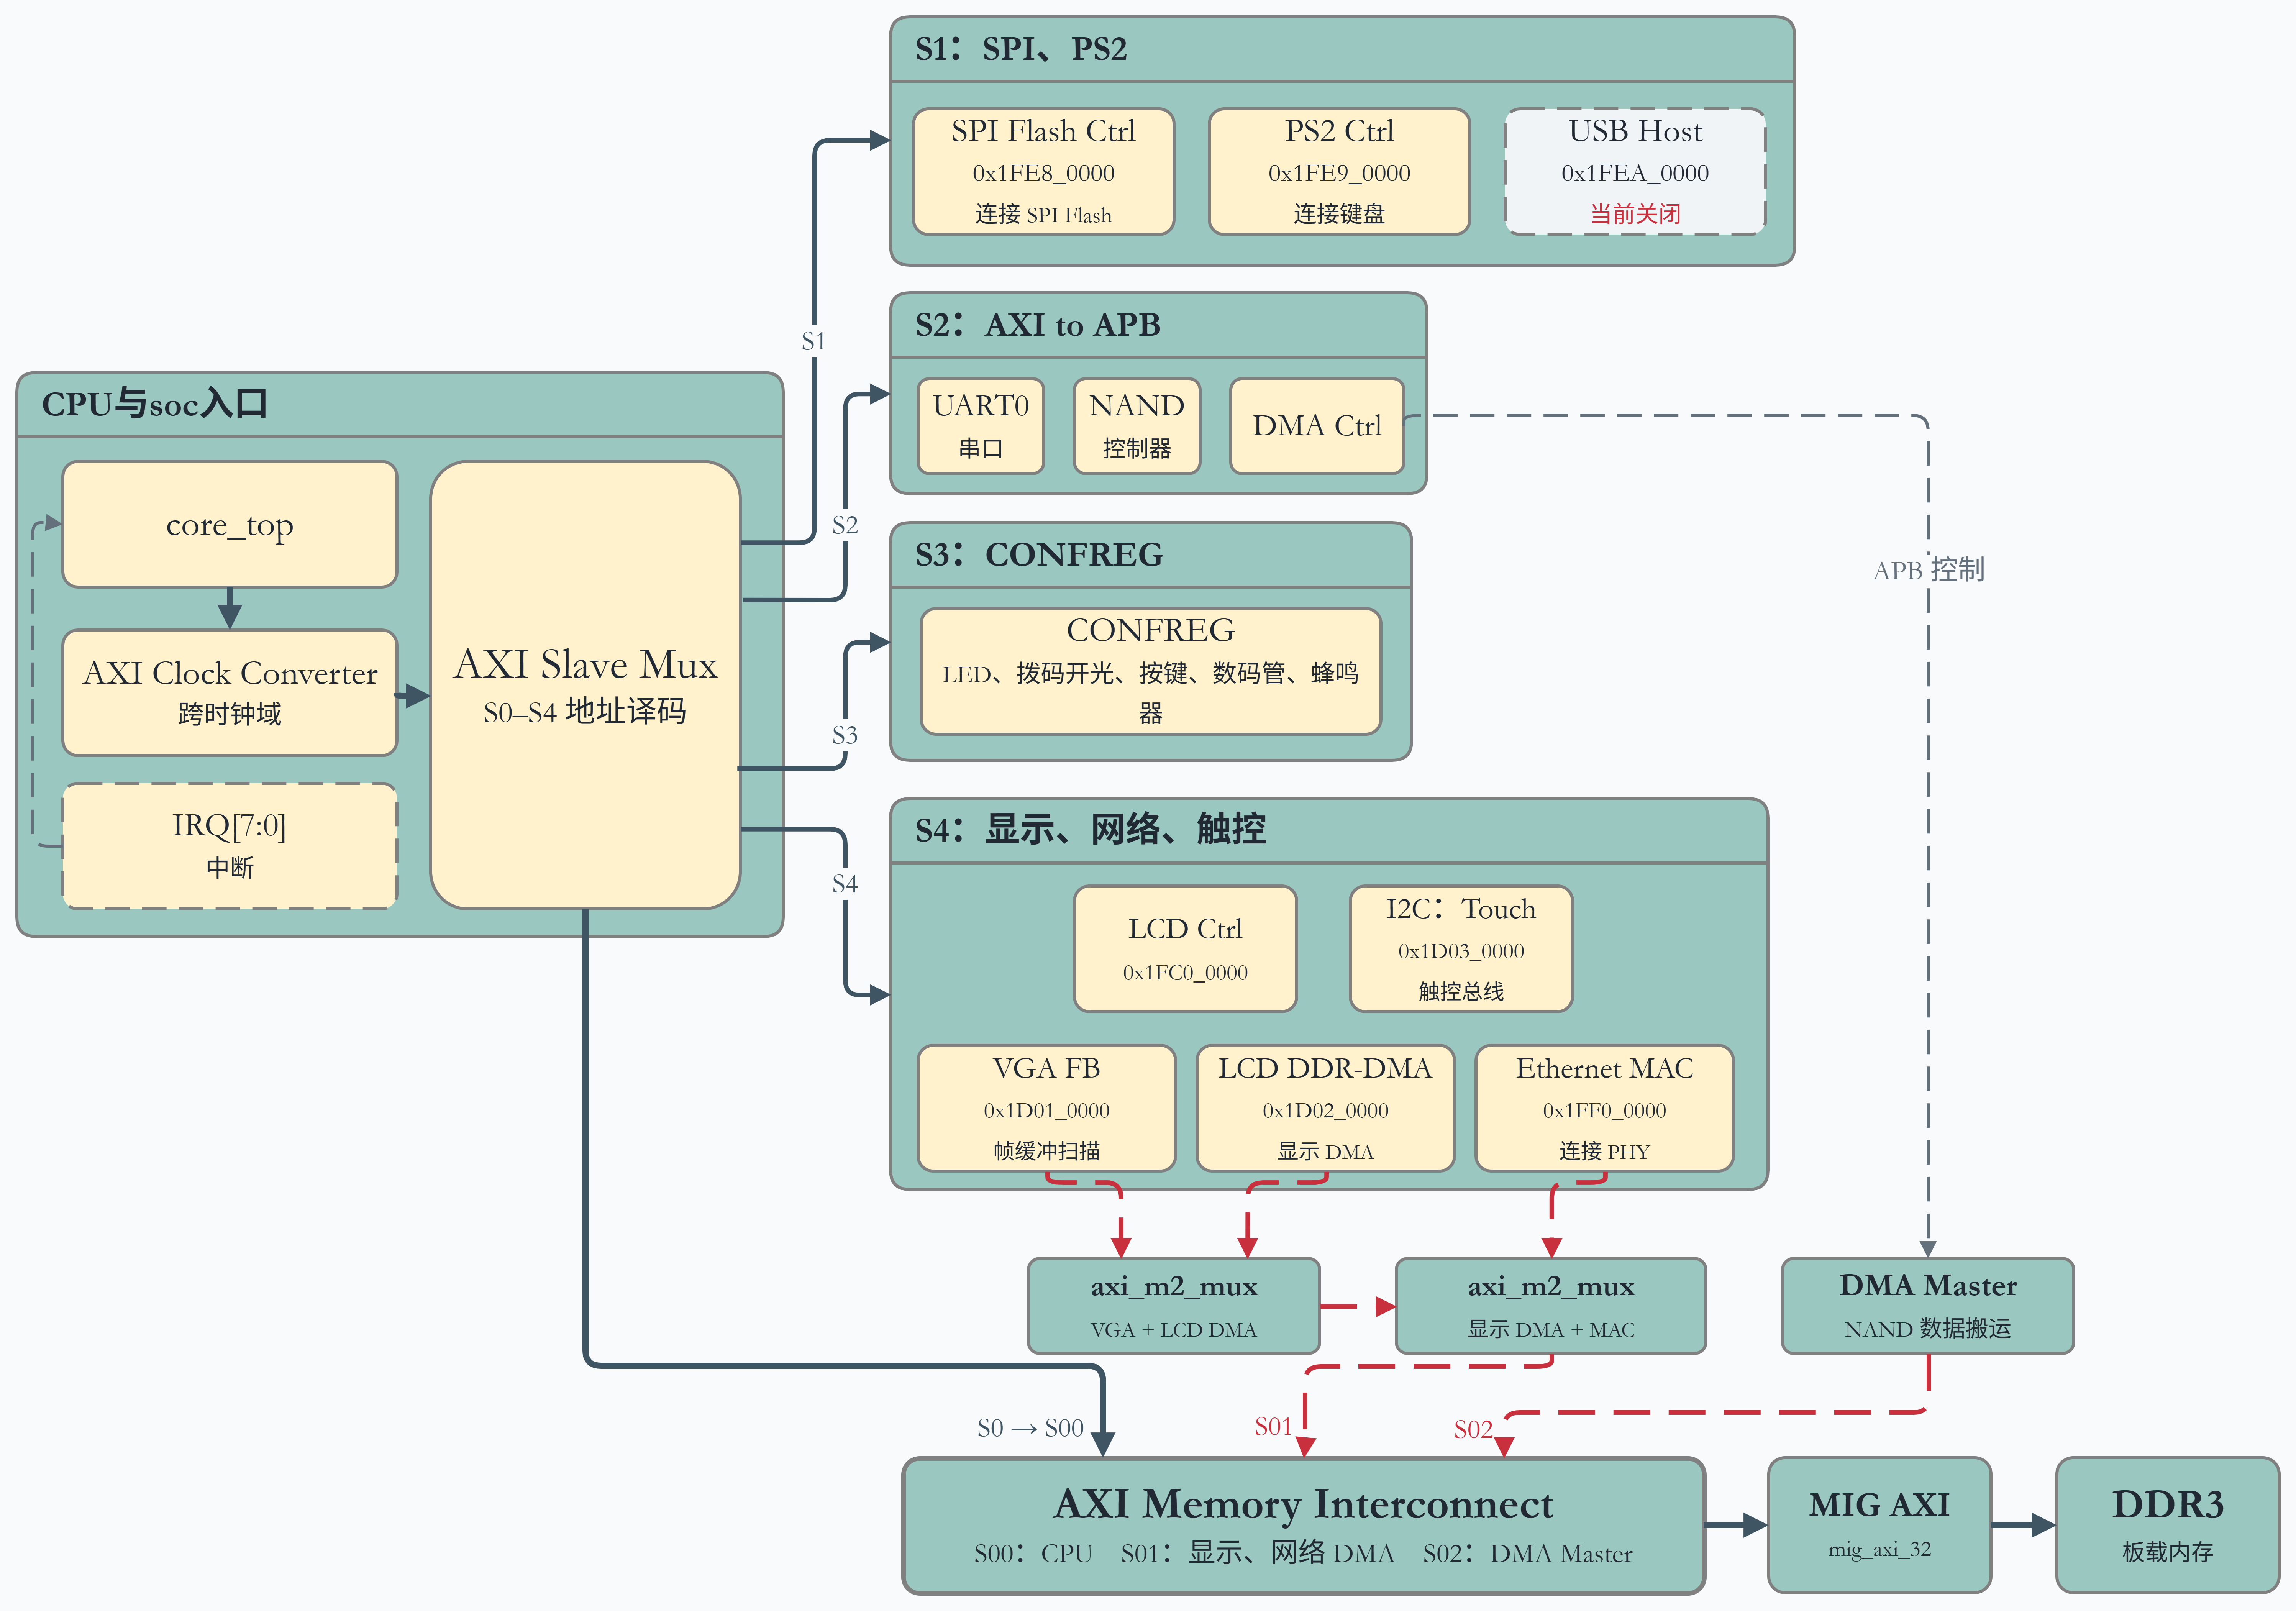
\includegraphics[width=0.95\textwidth]{figure/soc.png}
  \caption{soc架构图}
  \label{fig:soc}
\end{figure}

\subsubsection{互连、时钟与复位}

CPU AXI 经 AXI Clock Converter 进入 uncore 域，再由地址译码和 AXI/APB 互连分发至 DDR3、CONFREG 与各外设。DDR3 前端使用多主口互连，除 CPU 外，还承载 VGA/LCD/以太网 DMA 和 NAND/通用 DMA 流量。

\begin{table}[H]
\centering
\caption{SoC 主要时钟}
\label{tab:soc_clock}
\small
\begin{tabular}{lll}
\toprule
时钟 & 频率 & 用途 \\
\midrule
板级输入 & 100\,MHz & PLL 与时钟管理输入 \\
CPU & 60\,MHz & 处理器核与 CPU 侧 AXI \\
uncore & 60\,MHz & 外设、APB 与 SoC 主互连 \\
MIG 参考 & 200\,MHz & DDR3 PHY 参考 \\
MIG UI / DDR AXI & 100\,MHz & DDR3 用户接口 \\
VGA 像素 & 25\,MHz & 640$\times$480@60\,Hz 输出 \\
MII RX/TX 接口 & 25\,MHz & 以太网收发时钟 \\
\bottomrule
\end{tabular}
\end{table}

CPU 复位采用异步拉低、同步释放；DDR 相关逻辑还等待 PLL 锁定、MIG 校准完成和 UI 复位释放。PLL 失锁或 uncore 复位会重新复位 CPU 与跨时钟域桥，避免总线两侧进入不一致状态。

\subsubsection{地址分配}

\begin{table}[H]
\centering
\caption{SoC 主要物理地址映射}
\label{tab:addr}
\scriptsize
\begin{tabularx}{\textwidth}{>{\ttfamily}p{3.4cm}>{\raggedright\arraybackslash}p{3.2cm}X}
\toprule
地址 & 模块 & 说明 \\
\midrule
0x00000000--0x07FFFFFF & DDR3 & 128\,MiB 系统内存 \\
0x0A000000 & VGA Framebuffer & RGB565 默认 DMA 地址；经 MIG 低 27 位寻址别名至 DDR 0x02000000 \\
0x1C000000--0x1C0FFFFF & SPI Flash Window & 启动镜像和存储器访问窗口 \\
0x1D010000 & VGA Controller & DDR 帧缓冲显示控制 \\
0x1D020000 & LCD DMA & LCD 独立 DDR 读取通道 \\
0x1D030000 & I2C Master & 通用 I2C 与触摸共享总线 \\
0x1FC00000 区域 & LCD Controller & 8080 接口 LCD 控制，常用寄存器位于 0x1FC0C000 \\
0x1FD00000 区域 & CONFREG & GPIO、定时器、LED、数码管、按键、蜂鸣器与 DMA 控制 \\
0x1FE001E0 & UART & 16550 串口数据与控制端口 \\
0x1FE70000 区域 & NAND & NAND 控制器，Linux 节点使用 0x1FE78000 \\
0x1FE80000 & SPI Controller & SPI Flash 控制寄存器 \\
0x1FE90000 & PS/2 & 键盘/鼠标控制器 \\
0x1FEA0000 & USB Host & 保留窗口，当前工程未启用 \\
0x1FF00000 & Ethernet MAC & MII 10/100M MAC 与 DMA \\
\bottomrule
\end{tabularx}
\end{table}

地址译码未匹配的访问会落入 DDR 路径，而 MIG 仅使用低 27 位地址。软件将规范 DDR 可用范围限制为 128\,MiB，避免高地址别名。

\subsubsection{外设与中断}

我们的 SOC 集成 UART、SPI、NAND、PS/2、GPIO、定时器、LED、数码管、蜂鸣器、VGA、8080 LCD、I2C 与 MII Ethernet。USB Host RTL 和管脚接口仍保留，但配置宏关闭；EJTAG 与调试 UART 也只作为保留接口，不作为当前已完成的调试功能。

\begin{table}[H]
\centering
\caption{CPU 外部中断映射}
\label{tab:interrupt}
\small
\begin{tabular}{cl}
\toprule
CPU 中断位 & 中断源 \\
\midrule
0 & Ethernet MAC \\
1 & UART \\
2 & SPI \\
3 & NAND \\
4 & DMA \\
5 & PS/2 \\
6 & 保留；启用 USB Host 时可连接 USB \\
7 & 保留 \\
\bottomrule
\end{tabular}
\end{table}

所有 uncore 外设中断在送入 CPU 前经过两级同步。VGA 使用 640$\times$480@60\,Hz、RGB565 DDR 帧缓冲；LCD 使用 16 位 8080 接口并可由独立 DMA 从 DDR 读取图像。

\subsection{U-Boot 启动软件}

系统启动程序基于官方 U-Boot v2026.07，参考清华 JIT 团队的uboot优化，并针对我们的 SoC 完成板级移植。上电后由 FPGA MIG 完成 DDR3 初始化与校准，处理器随后从 SPI Flash 启动；U-Boot 初始化直接映射窗口、Cache、串口与网络设备，确认并使用 128\,MiB SDRAM，将自身从 Flash 执行区重定位到 SDRAM，最终进入 \texttt{u-boot@LoongsonSoC\#} 命令行。

\subsubsection{板级适配}

主要适配内容包括：
\begin{itemize}
  \item LA32R 启动入口、重定位、Cache 初始化、计时器和 16550 串口；
  \item 128\,MiB SDRAM 容量识别与重定位、SPI Flash、非 PCI DC2114x Ethernet MAC 与板级设备树；
  \item 非一致 DMA 所需的 cached/uncached DMW 地址转换和 \texttt{dbar} 所有权屏障；
  \item Linux ELF 装载和跳转前的 Cache 清理、屏障与启动参数传递。
\end{itemize}

当前网络驱动使用 32 个 RX descriptor 与 4 个 TX descriptor，配置 full-duplex、store-and-forward 和发送阈值；RX packet buffer 使用 uncached 映射，避免每包重复 Cache sweep。TFTP 默认块大小为 1468\,B、窗口大小为 1。当前 SoC 没有 SD/MMC 控制器、引脚或设备树节点，因此启动路径不包含 SD 卡。

\subsubsection{TFTP 启动 Linux}
U-Boot 2026.07 已在 CPU 为 60\,MHz 的当前 SoC 上完成实际启动，并可通过串口进入命令行、通过 TFTP 加载 Linux 镜像。TFTP 加载速度高达 500 KB/s。

\begin{figure}[H]
  \centering
  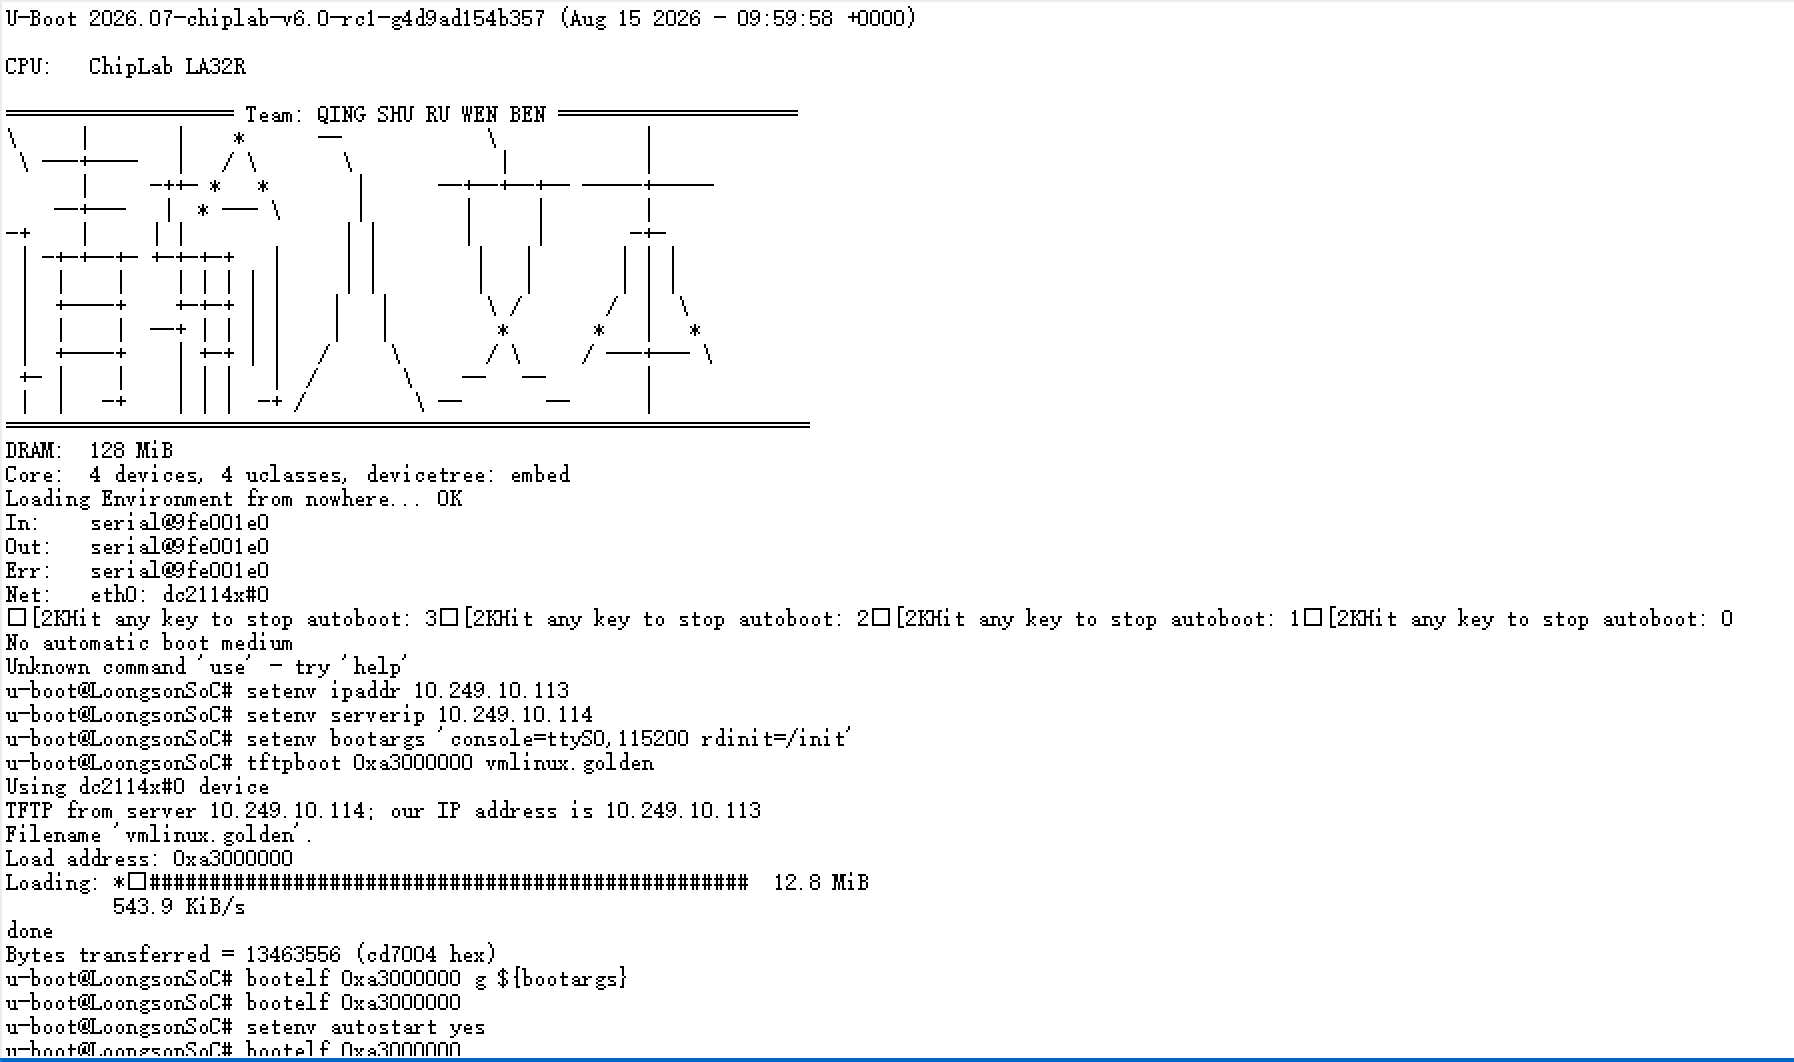
\includegraphics[width=0.95\textwidth]{figure/uboot.png}
  \caption{uboot启动linux}
  \label{fig:uboot}
\end{figure}

\subsection{Linux 系统}

我们致力于搭建一个具有较完善 GUI 系统和丰富软件生态的 Linux 系统。

\begin{figure}[H]
  \centering
  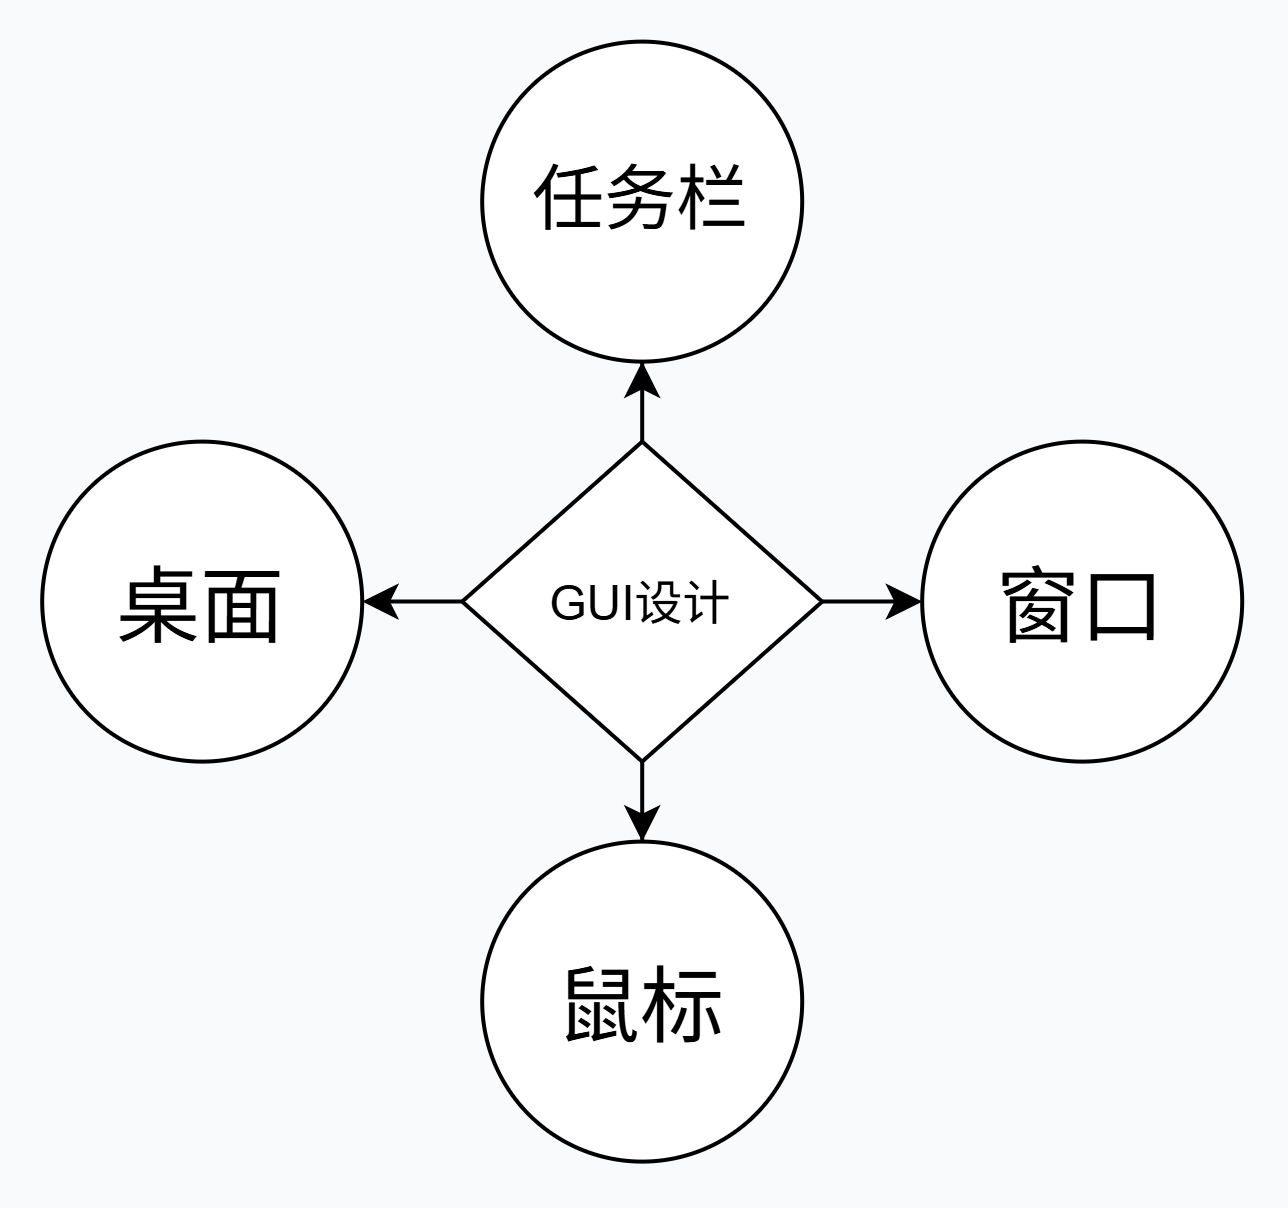
\includegraphics[width=0.5\textwidth]{figure/GUI.png}
  \caption{GUI}
  \label{fig:GUI}
\end{figure}

\begin{figure}[H]
  \centering
  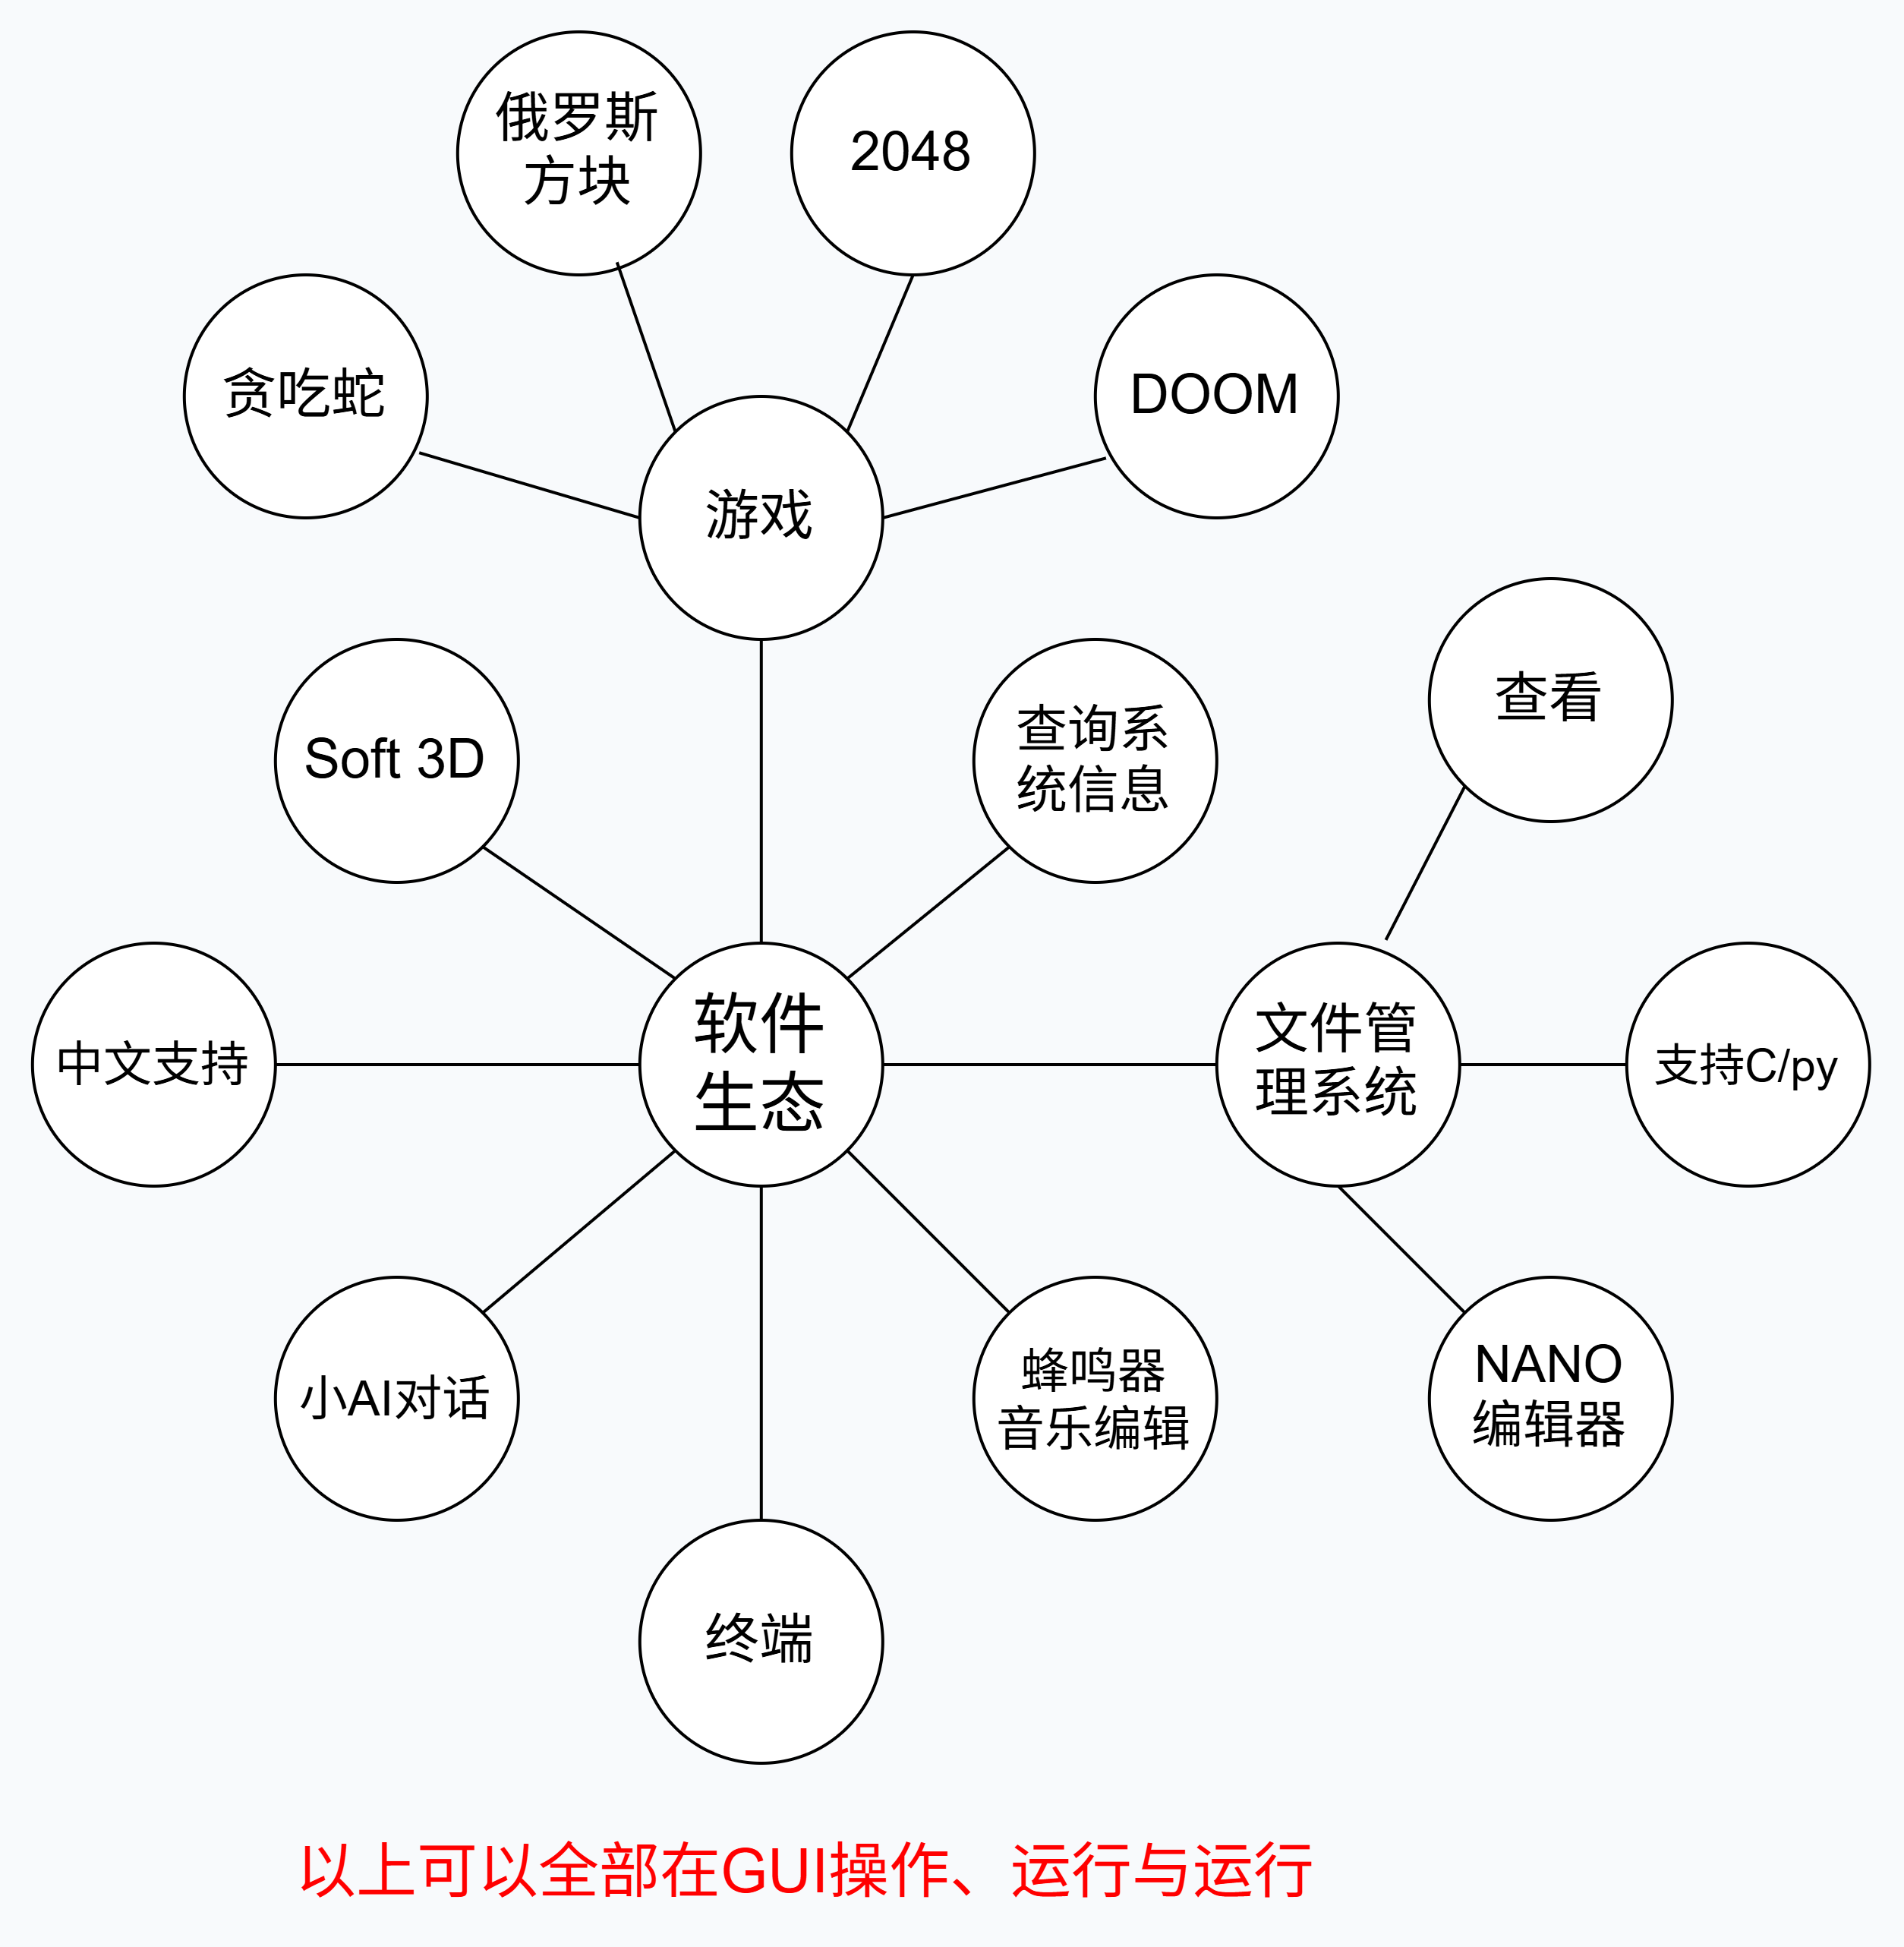
\includegraphics[width=0.95\textwidth]{figure/软件生态.png}
  \caption{软件生态}
  \label{fig:软件生态}
\end{figure}

\subsubsection{GUI展示}

我们的GUI支持完整的桌面、鼠标（ LCD 控制）、任务栏、时间、多窗口、鼠标拖拽等设计。如下：

\begin{figure}[H]
  \centering
  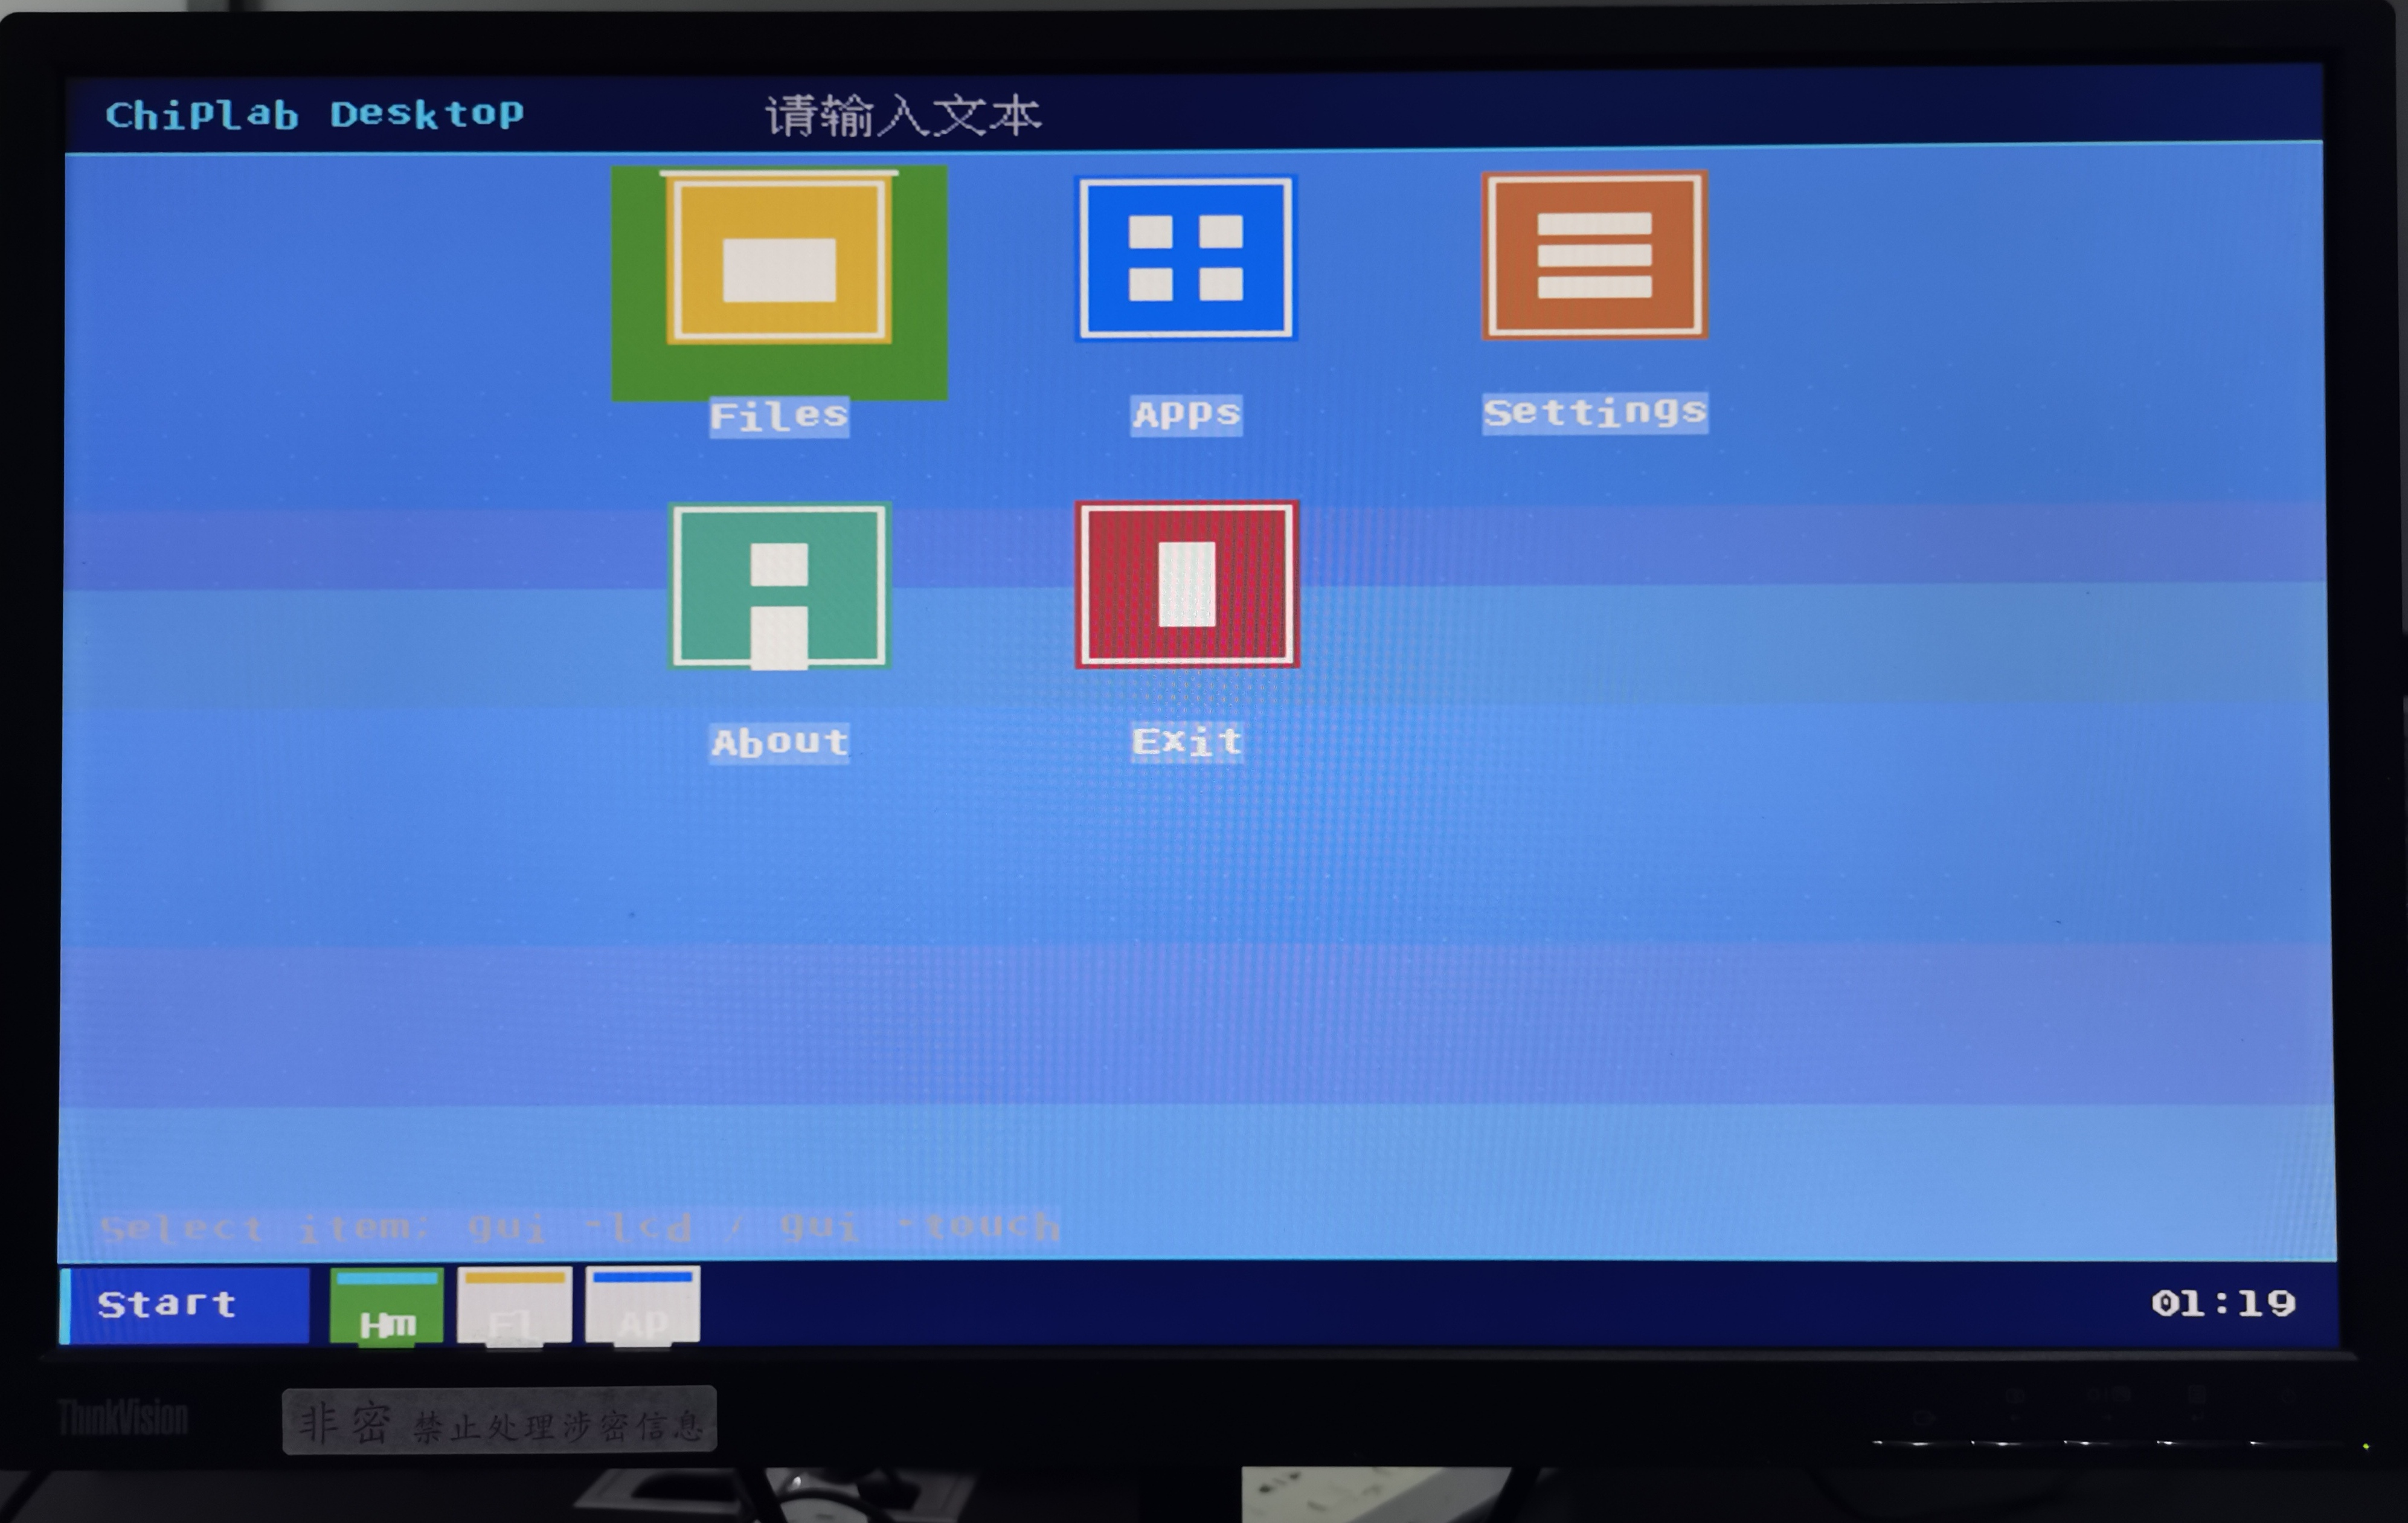
\includegraphics[width=0.95\textwidth]{figure/GUI桌面.jpg}
  \caption{GUI 桌面}
  \label{fig:GUI 桌面}
\end{figure}

\begin{figure}[H]
  \centering
  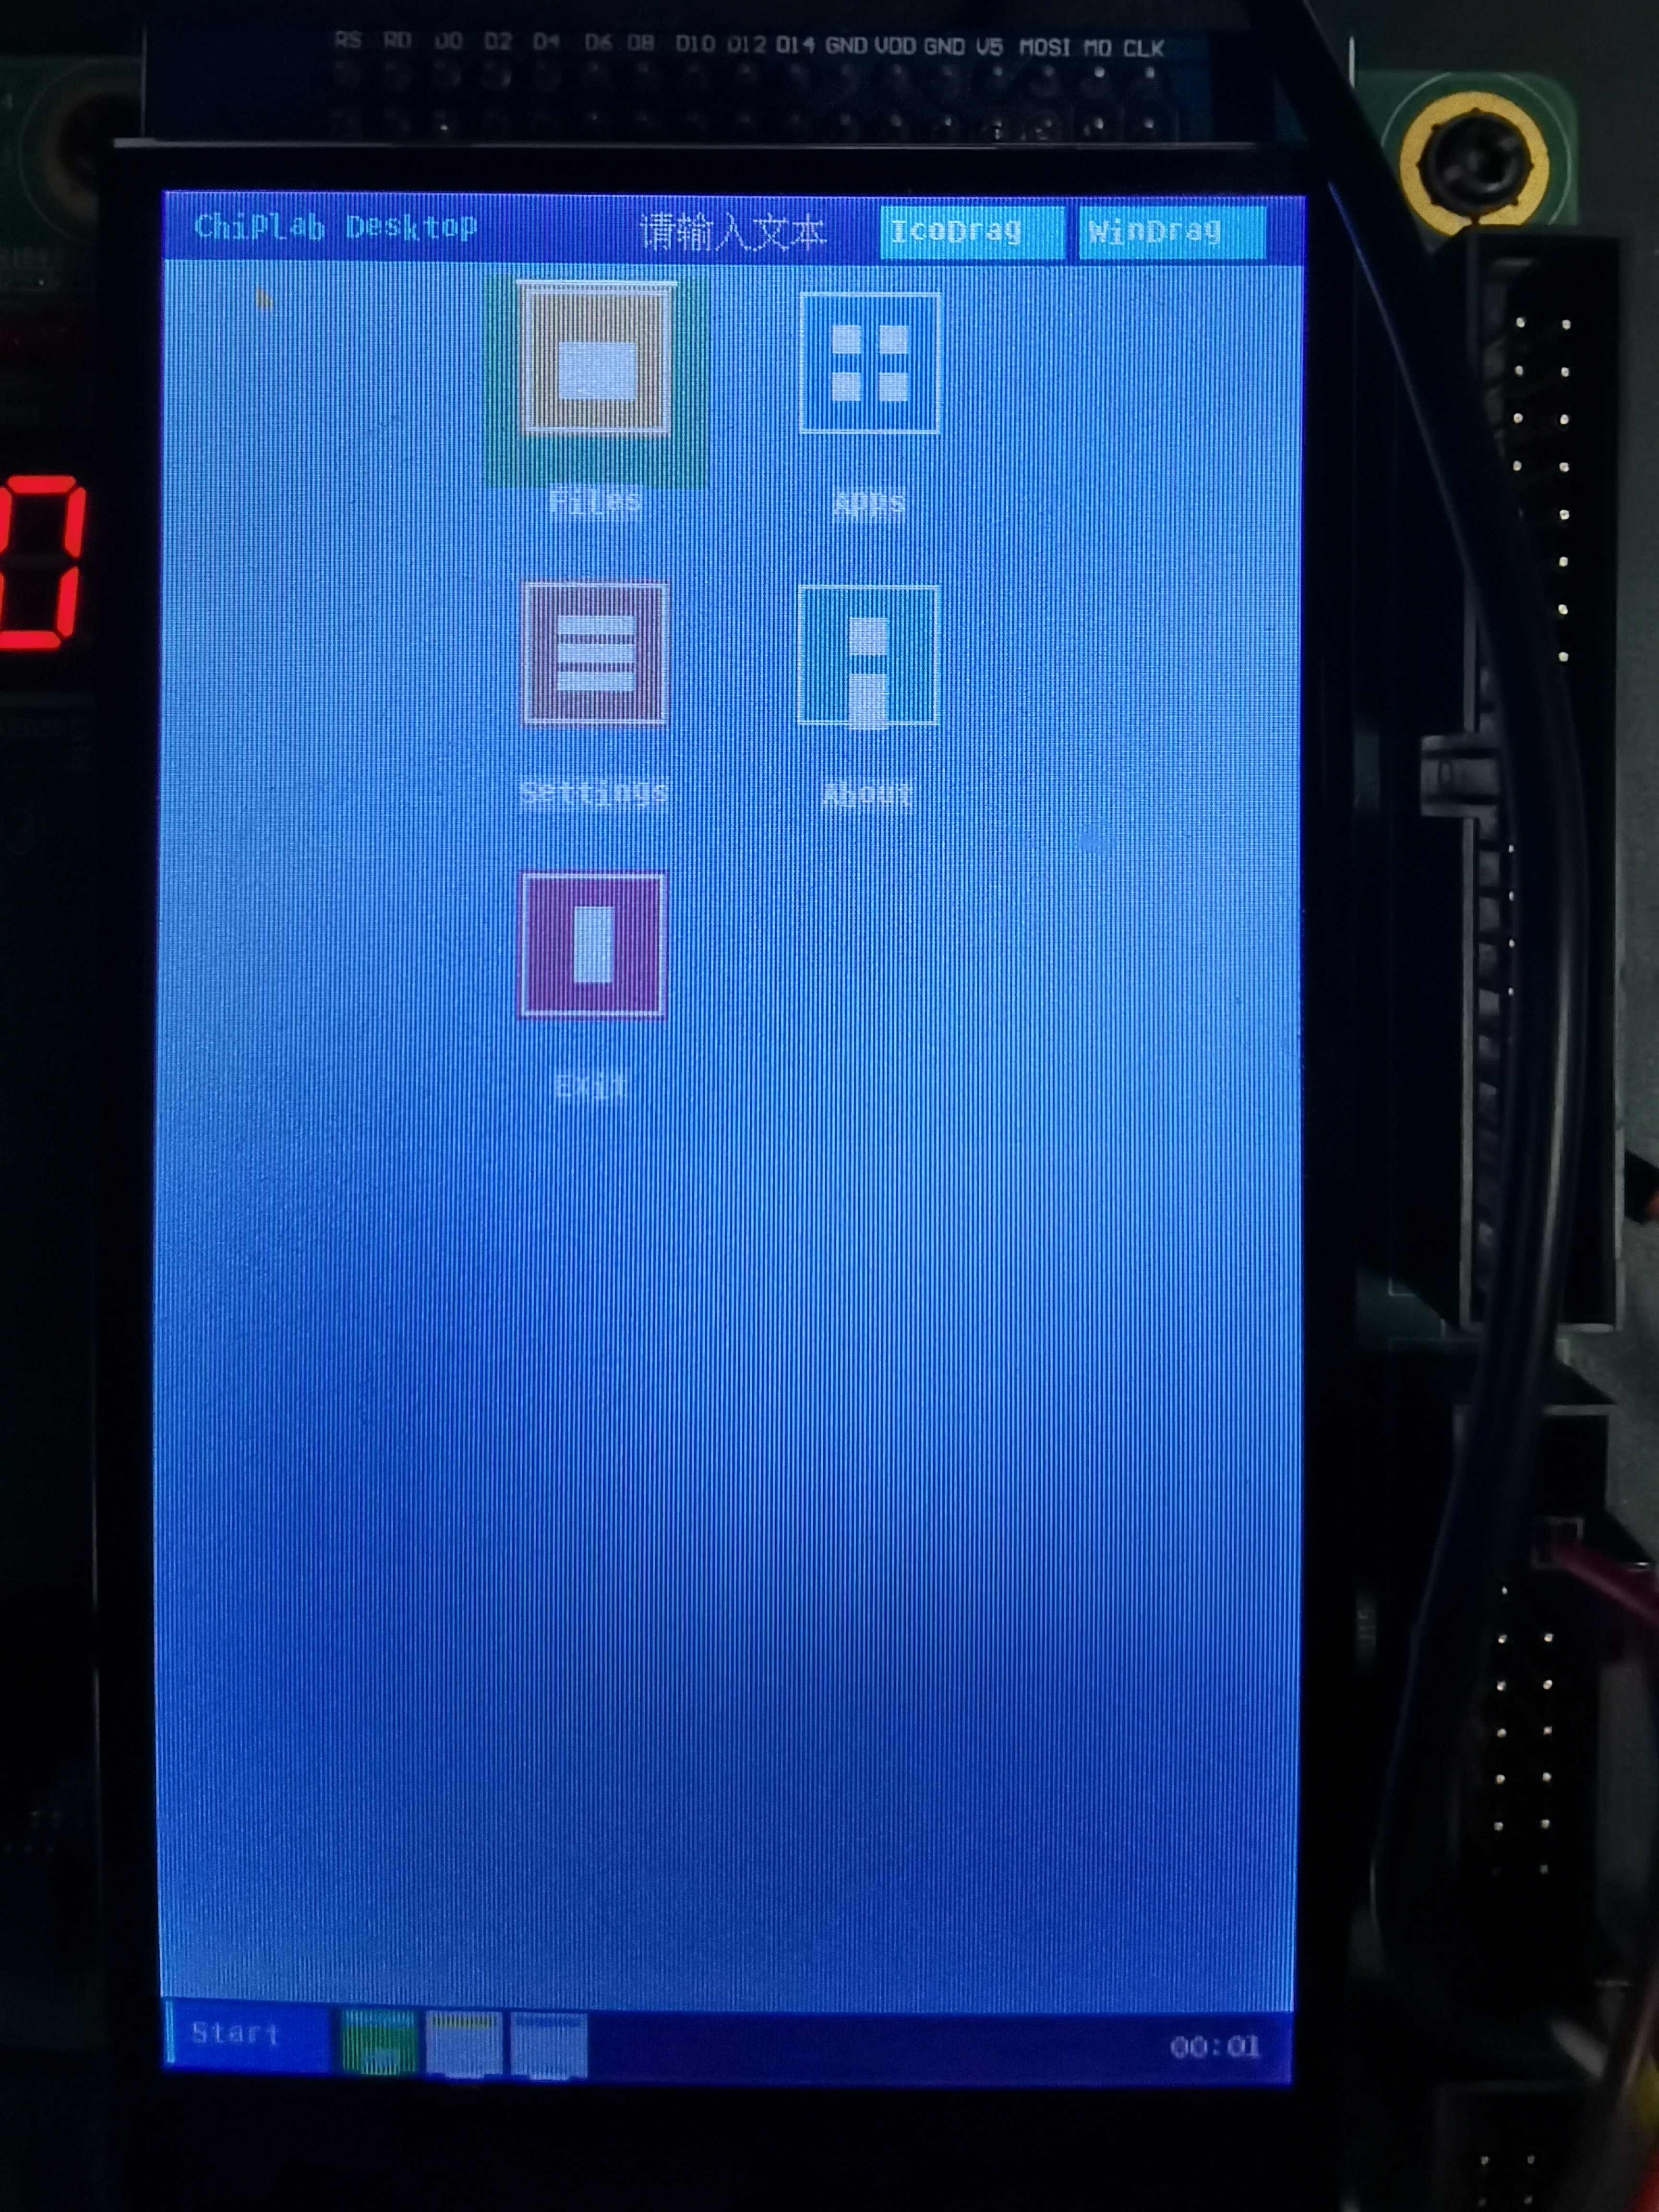
\includegraphics[width=0.3\textwidth]{figure/LCD_GUI.jpg}
  \caption{LCD GUI}
  \label{fig:LCD GUI}
\end{figure}

\begin{figure}[H]
  \centering
  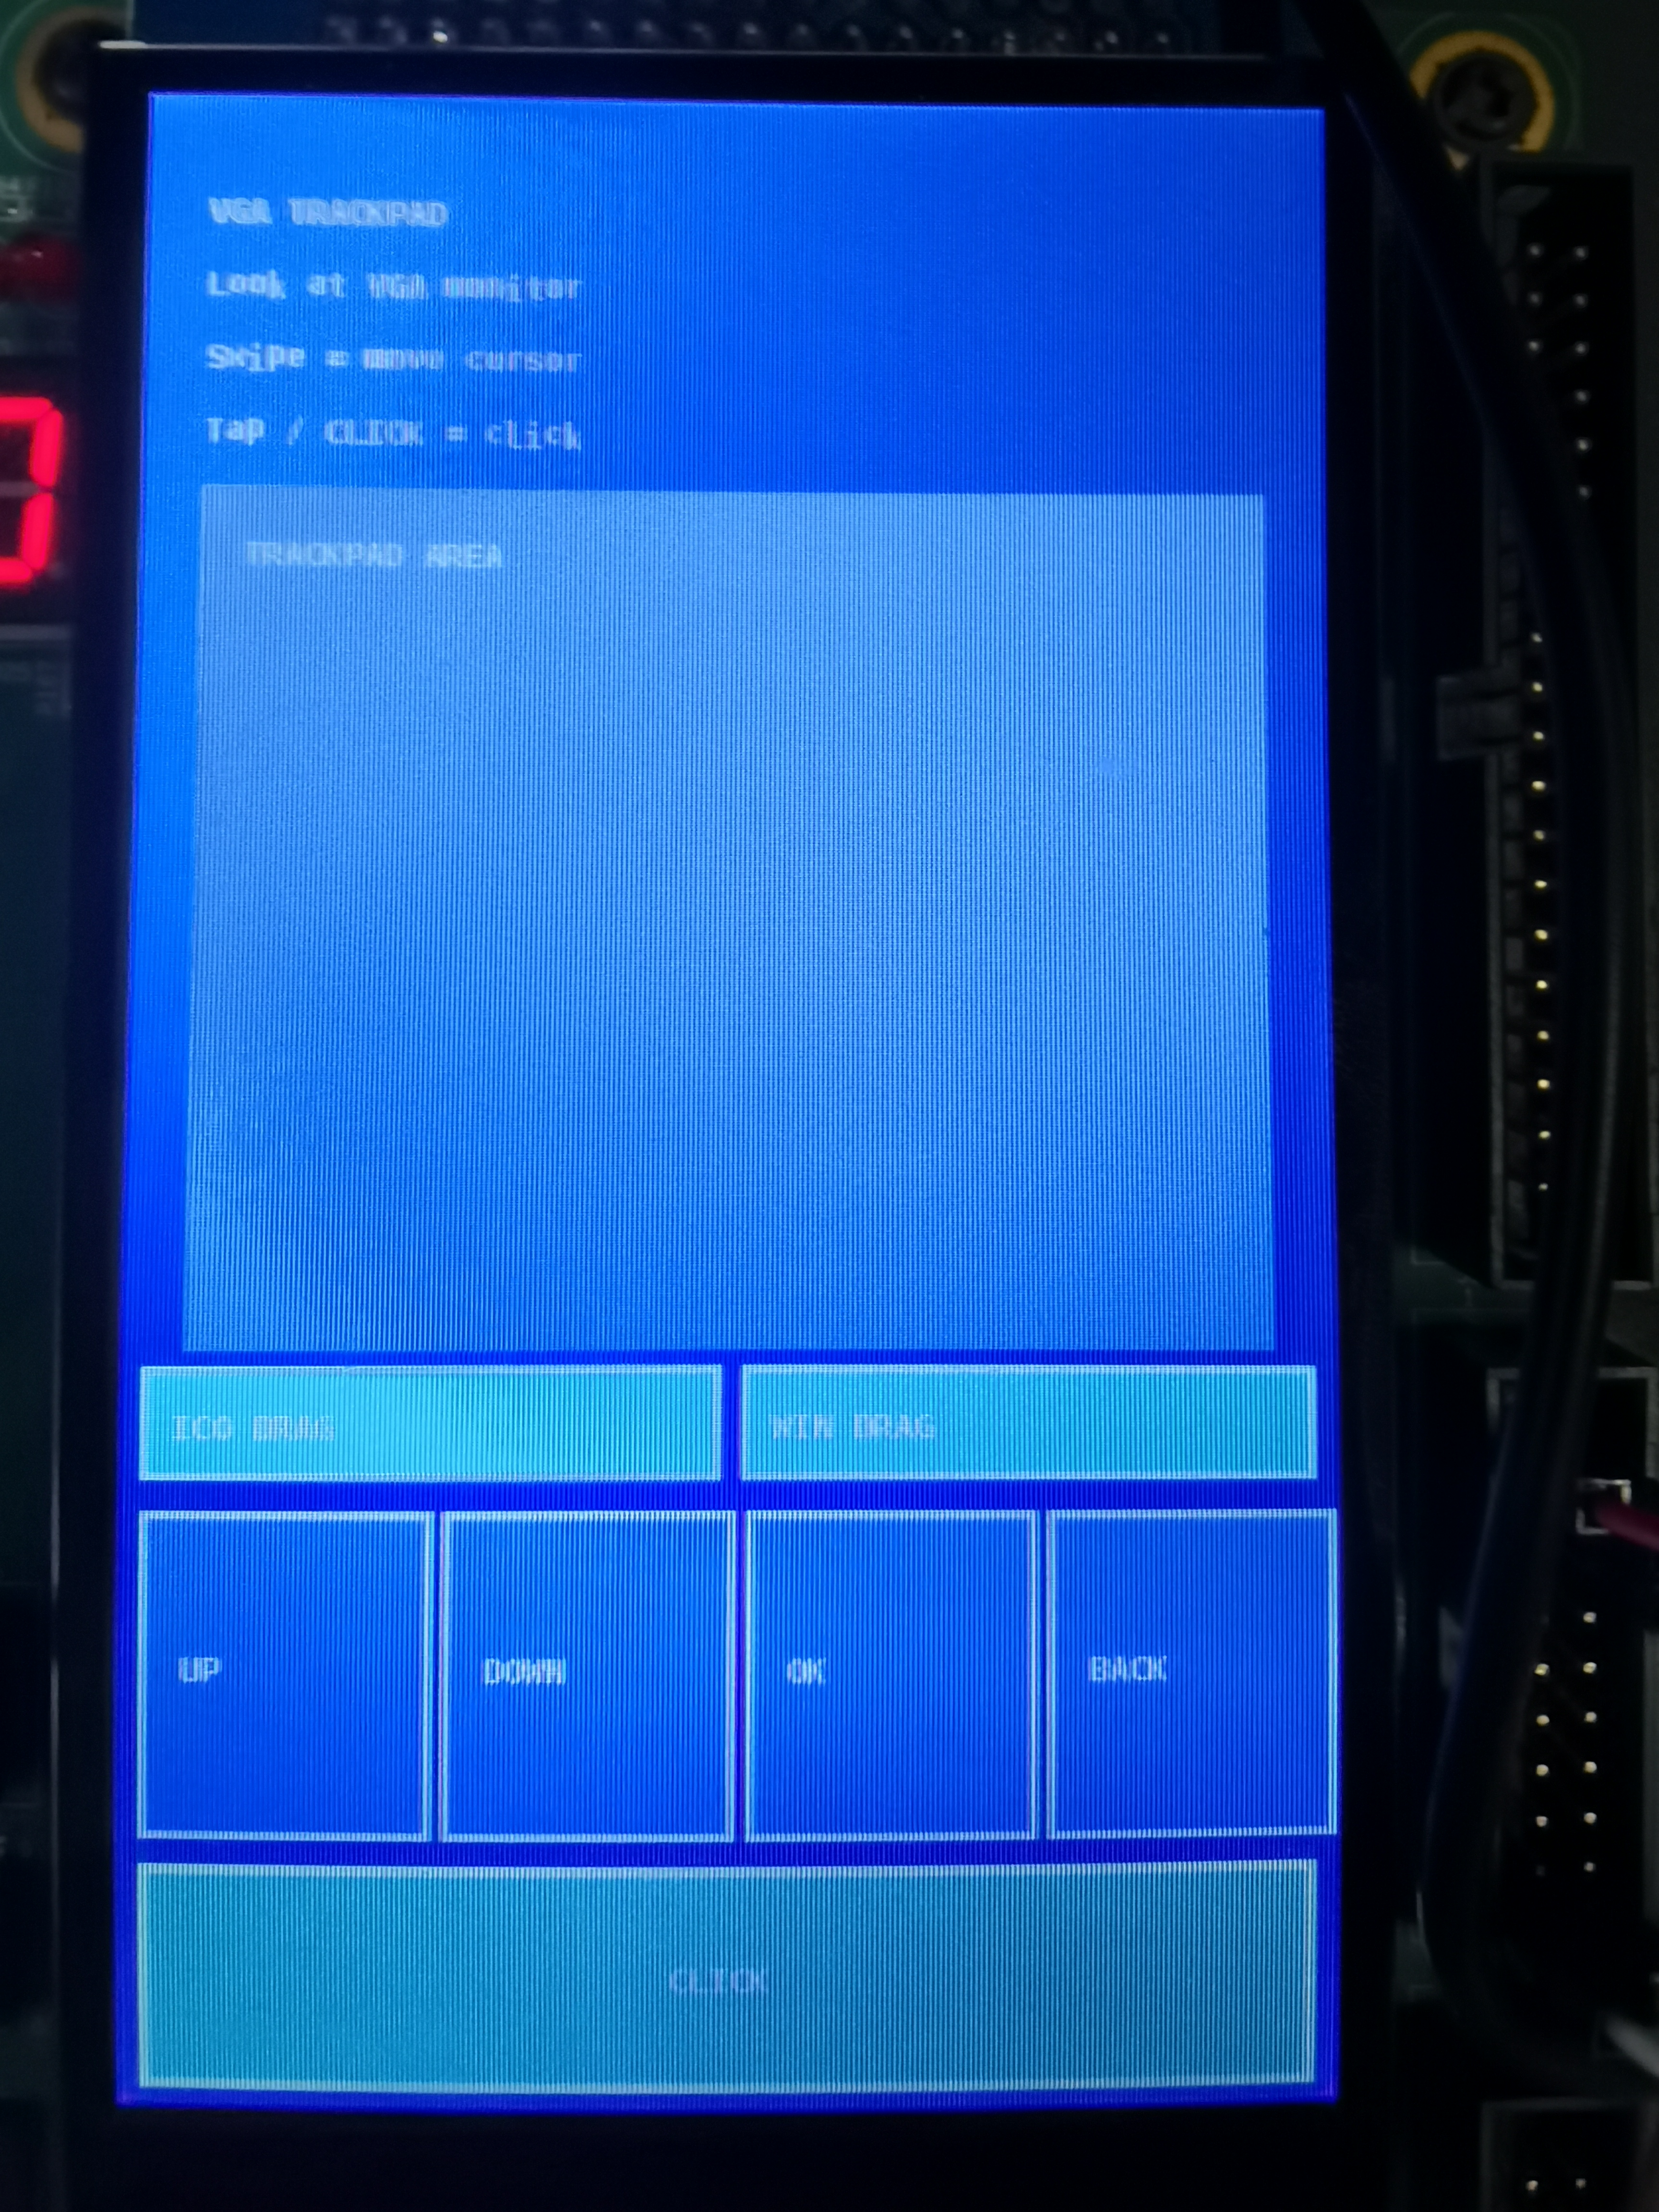
\includegraphics[width=0.3\textwidth]{figure/LCD_Mouse.jpg}
  \caption{LCD Mouse}
  \label{fig:LCD Mouse}
\end{figure}

\begin{figure}[H]
  \centering
  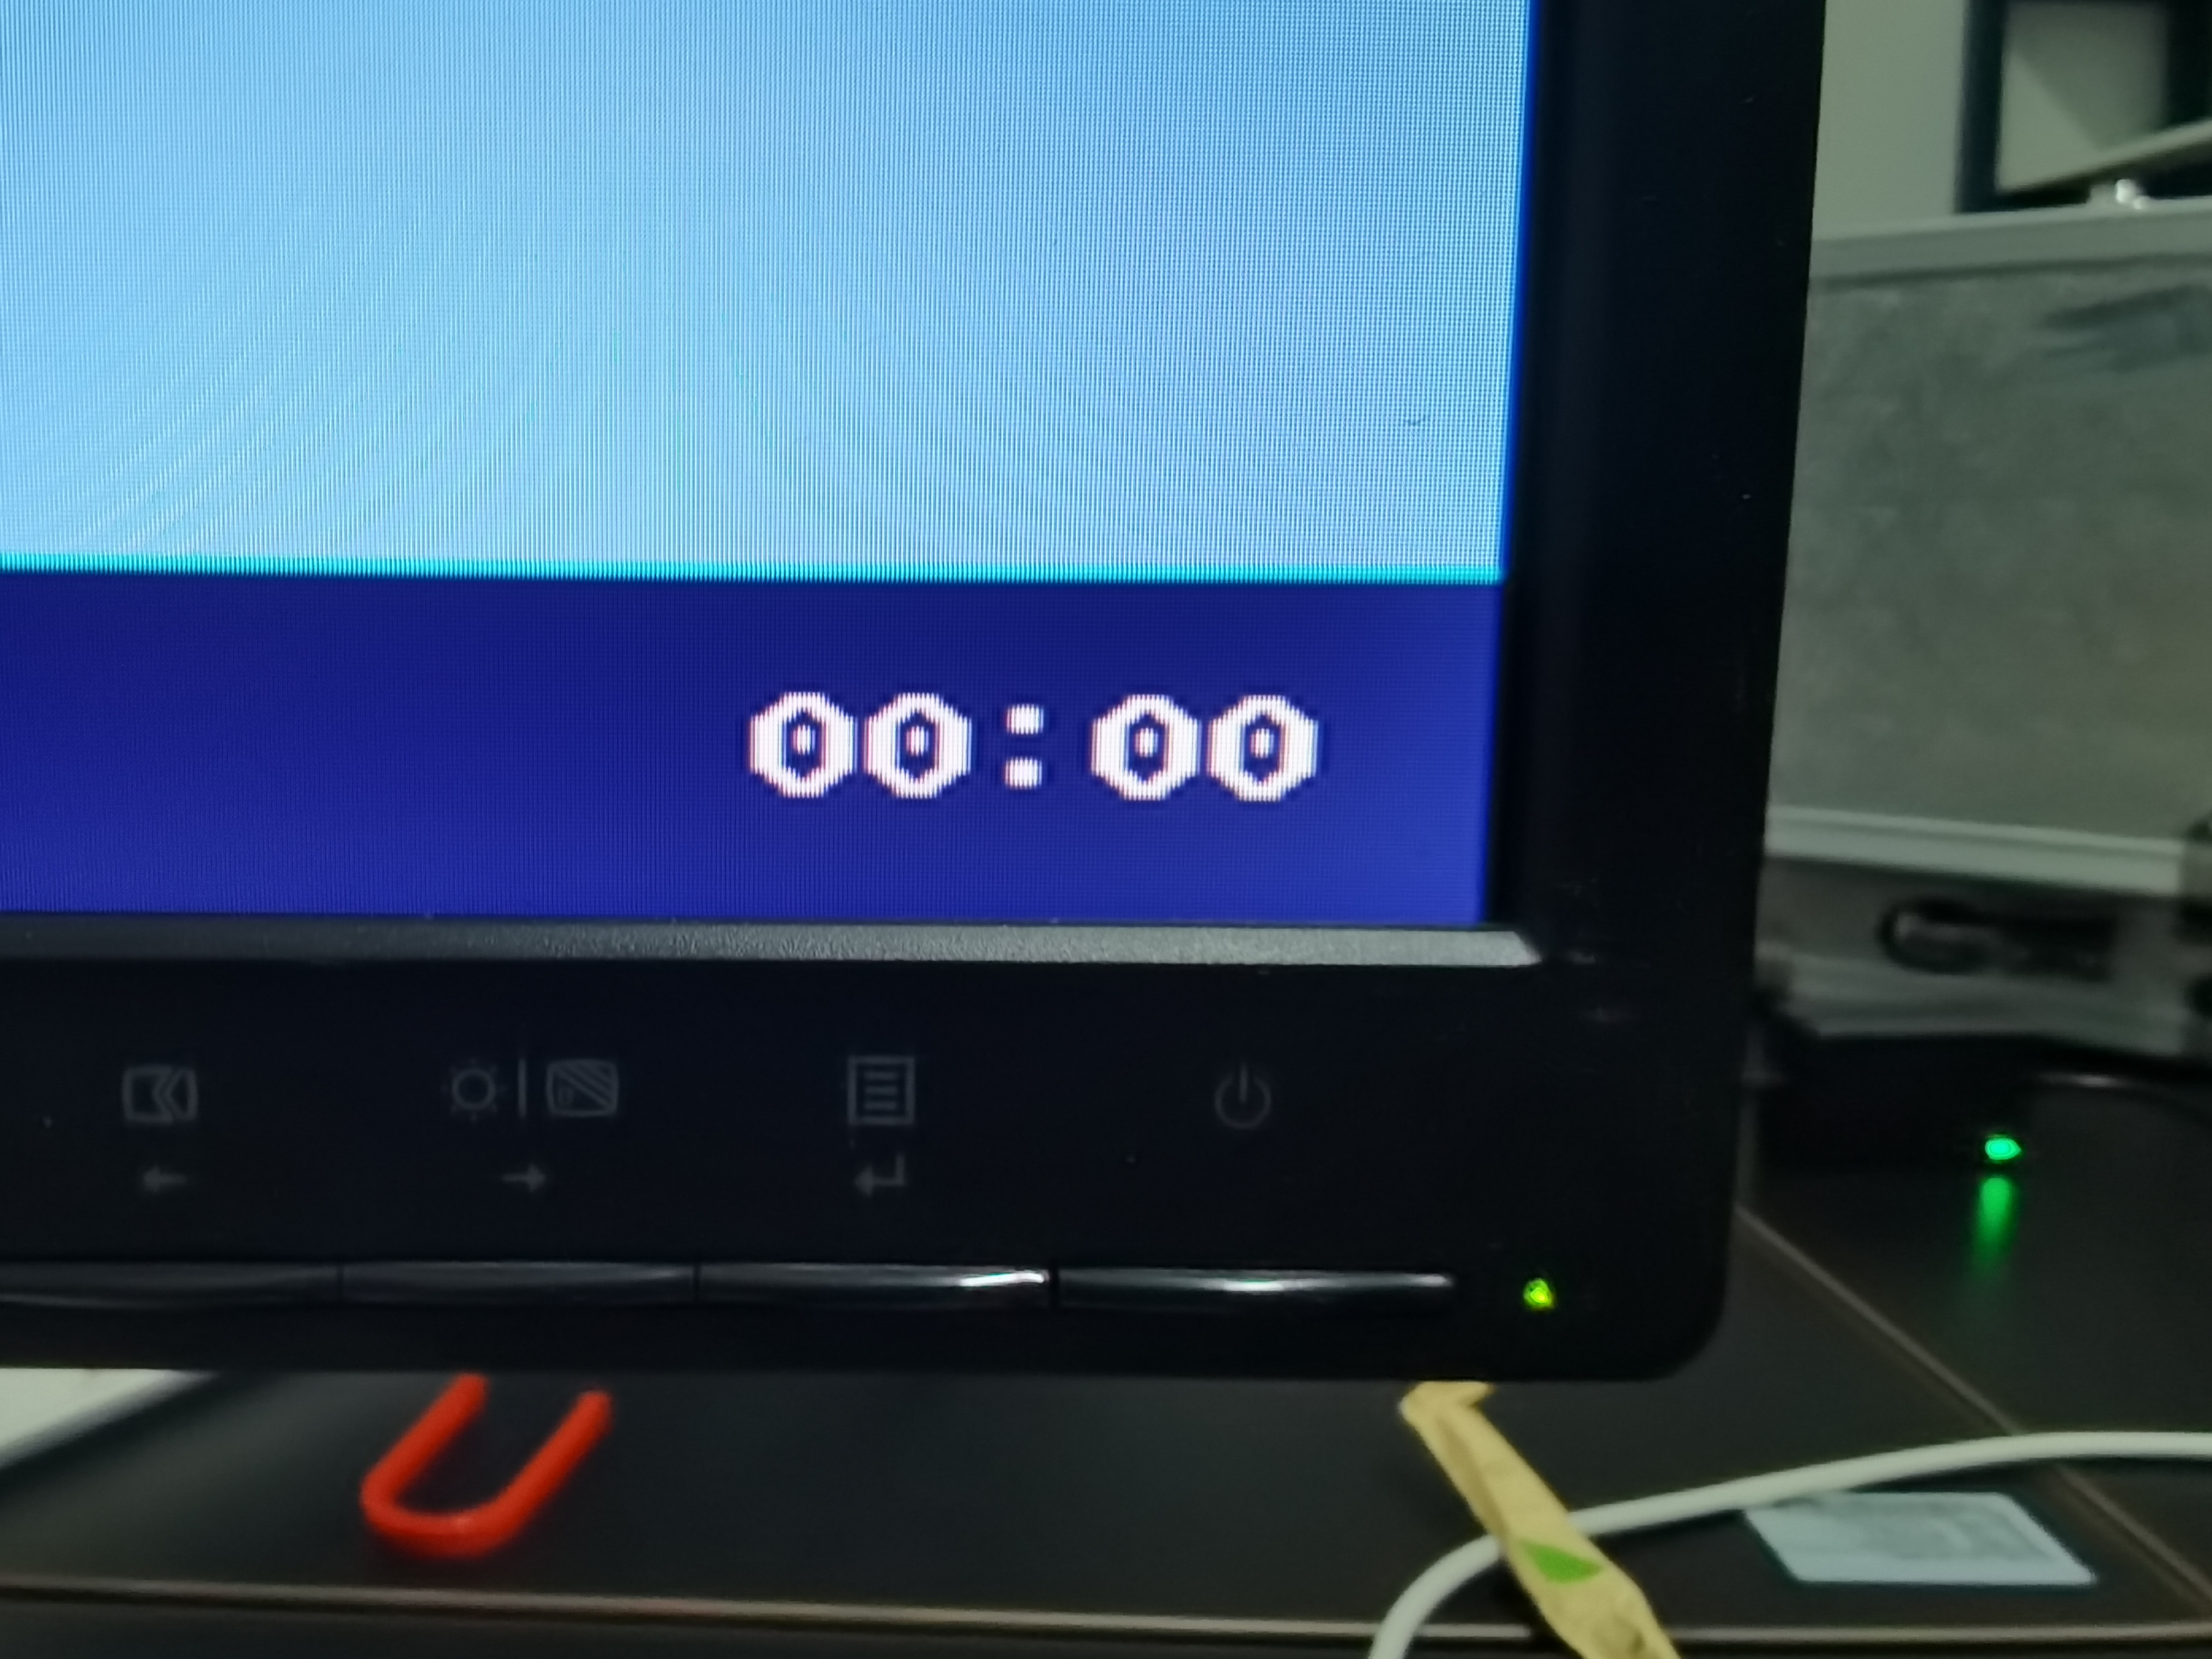
\includegraphics[width=0.3\textwidth]{figure/LCD_Time.jpg}
  \caption{LCD Time}
  \label{fig:LCD Time}
\end{figure}

\begin{figure}[H]
  \centering
  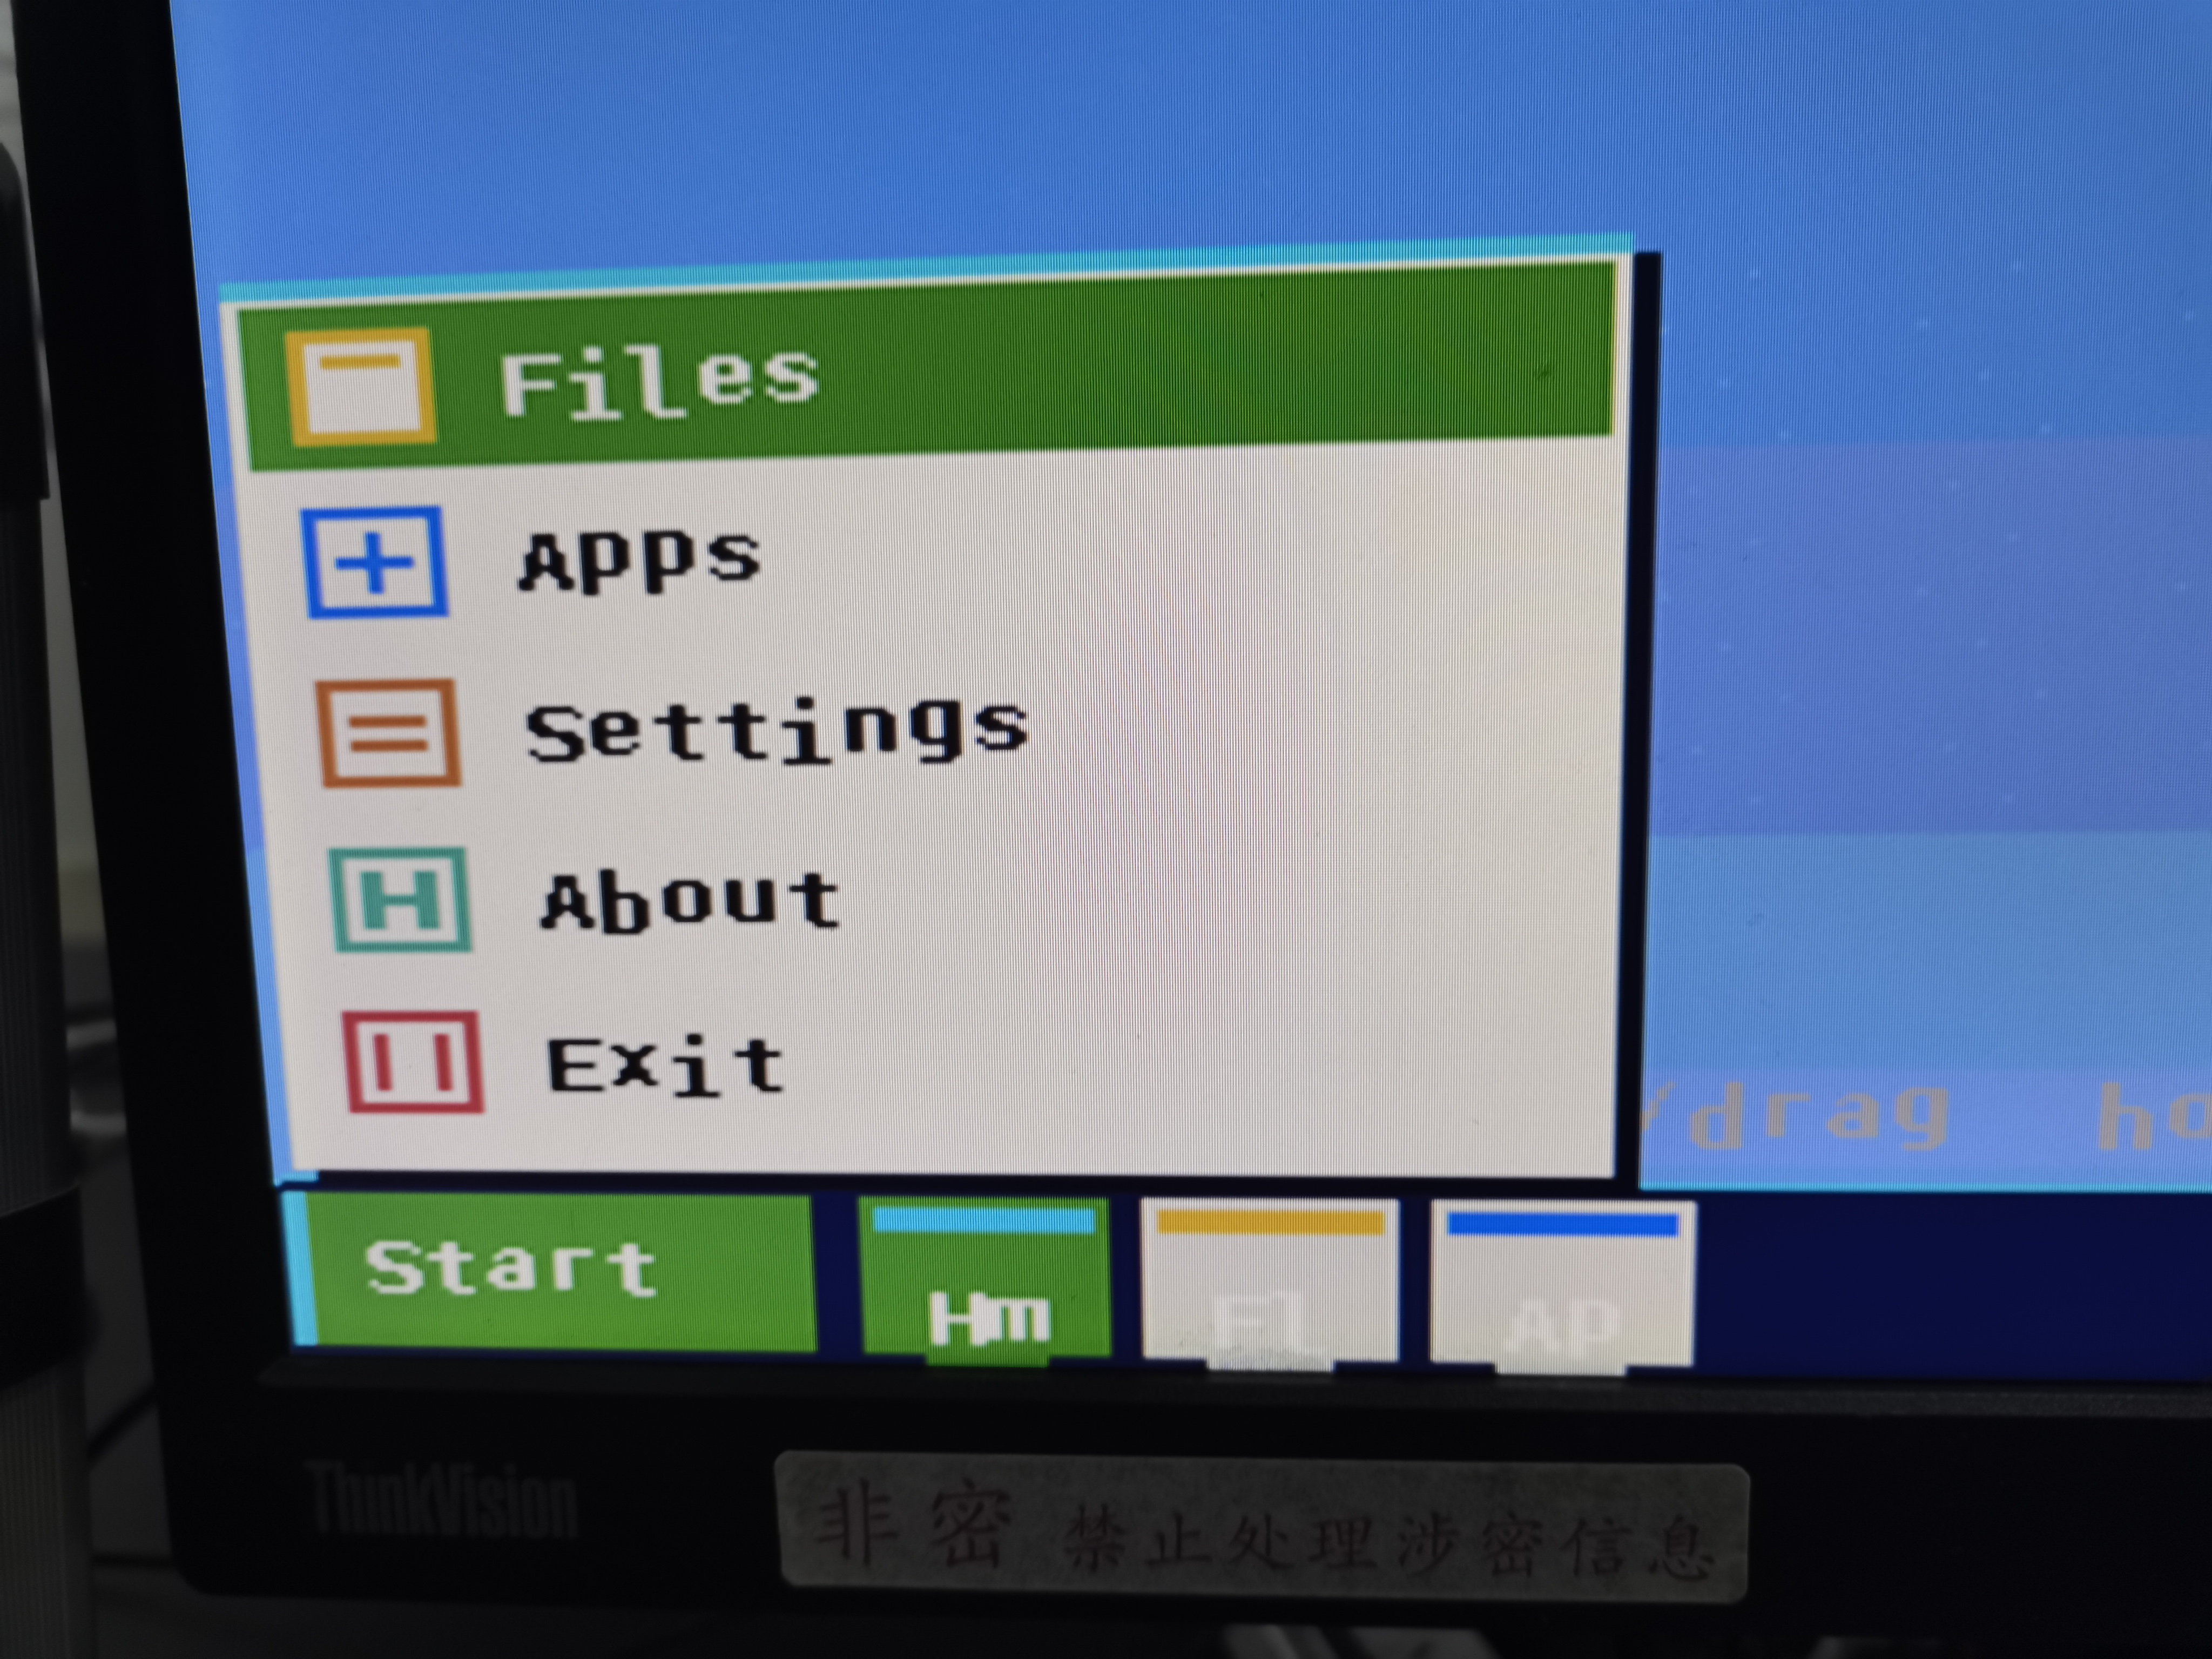
\includegraphics[width=0.3\textwidth]{figure/菜单栏.jpg}
  \caption{菜单栏}
  \label{fig:菜单栏}
\end{figure}

\begin{figure}[H]
  \centering
  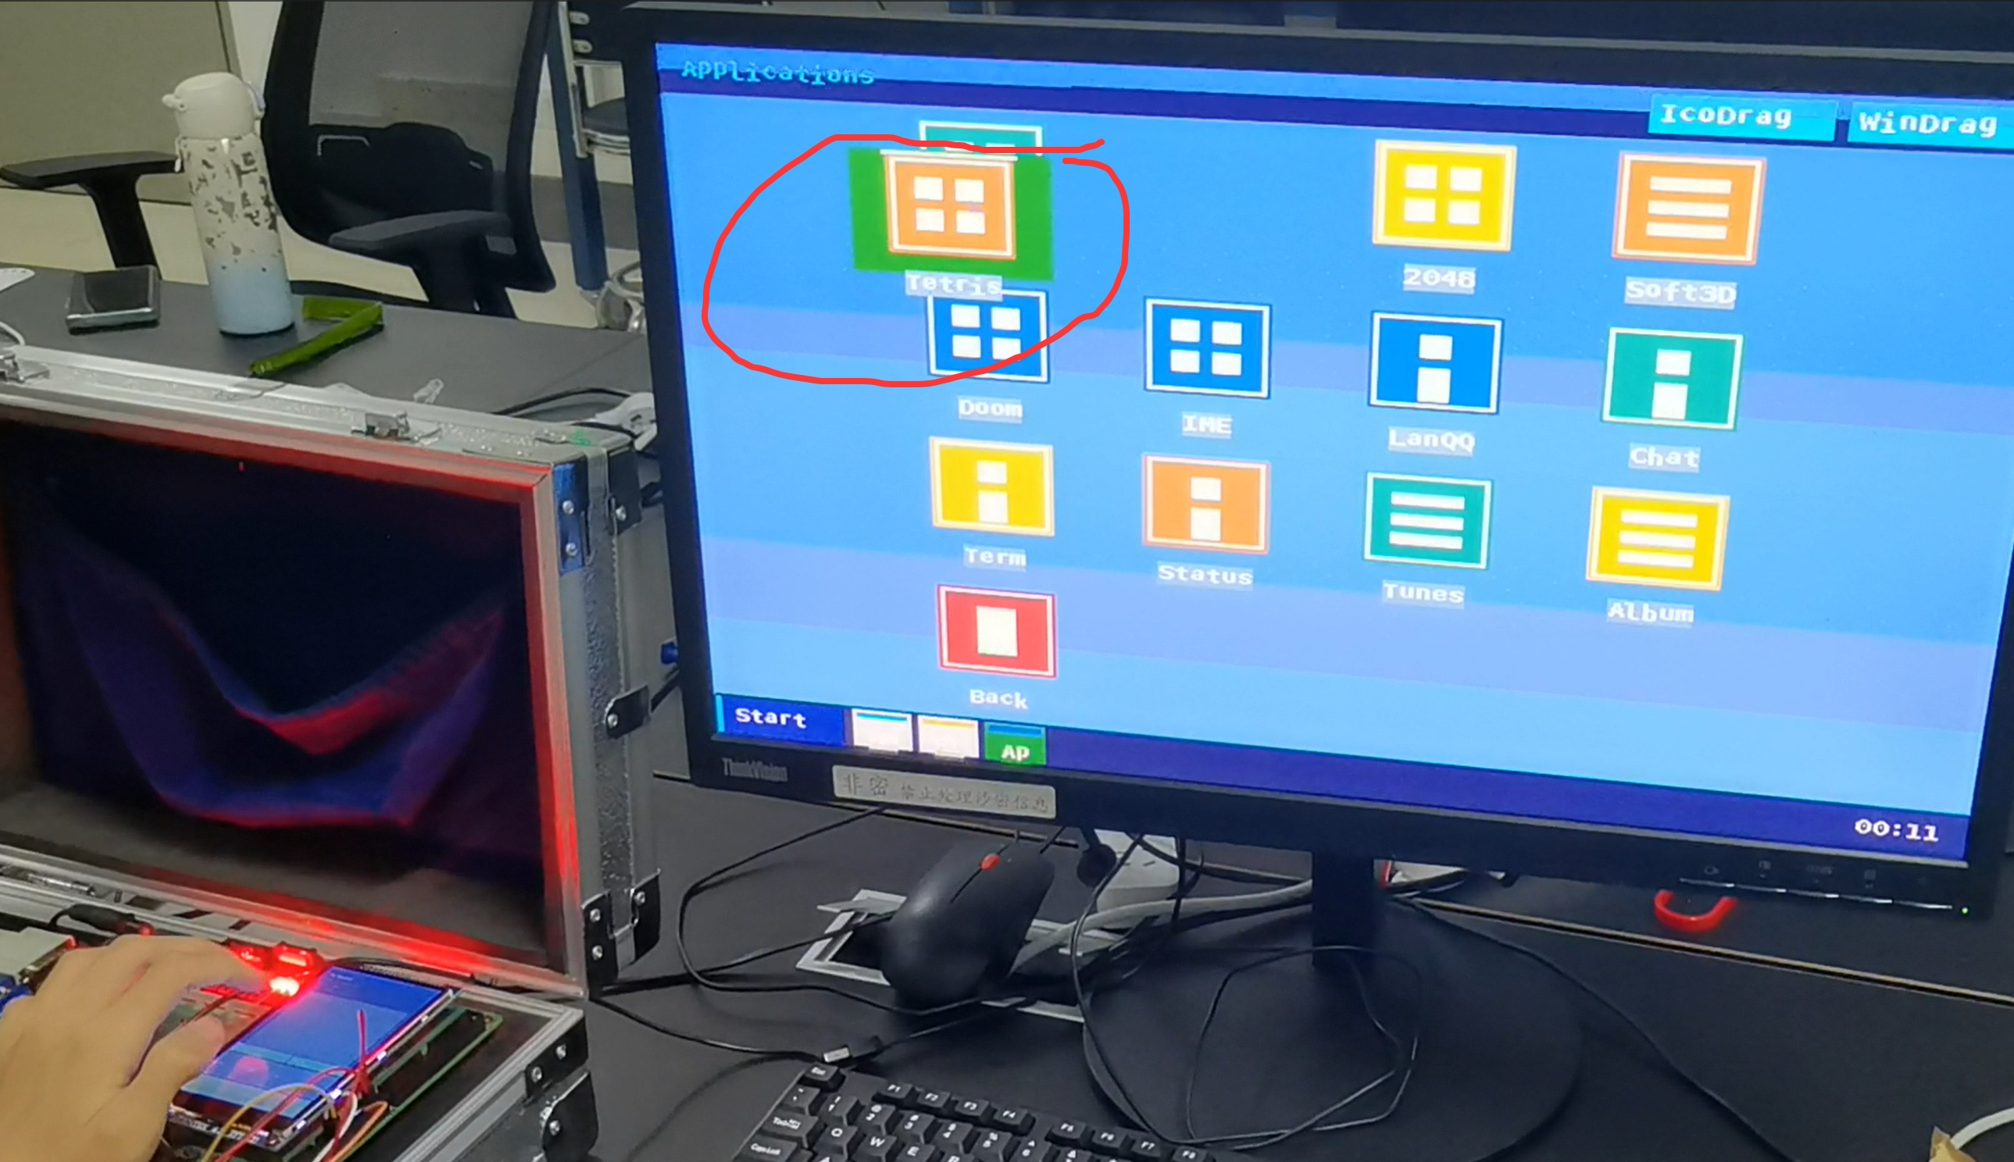
\includegraphics[width=0.95\textwidth]{figure/鼠标拖拽.png}
  \caption{鼠标拖拽}
  \label{fig:鼠标拖拽}
\end{figure}

\subsubsection{软件生态}

我们的 linux 系统支持多种游戏（包括 DOOM）、软浮点 3D 渲染、中文支持、小型意图推理模型、 NANO 编辑、 C/py 编译等。

\begin{figure}[H]
  \centering
  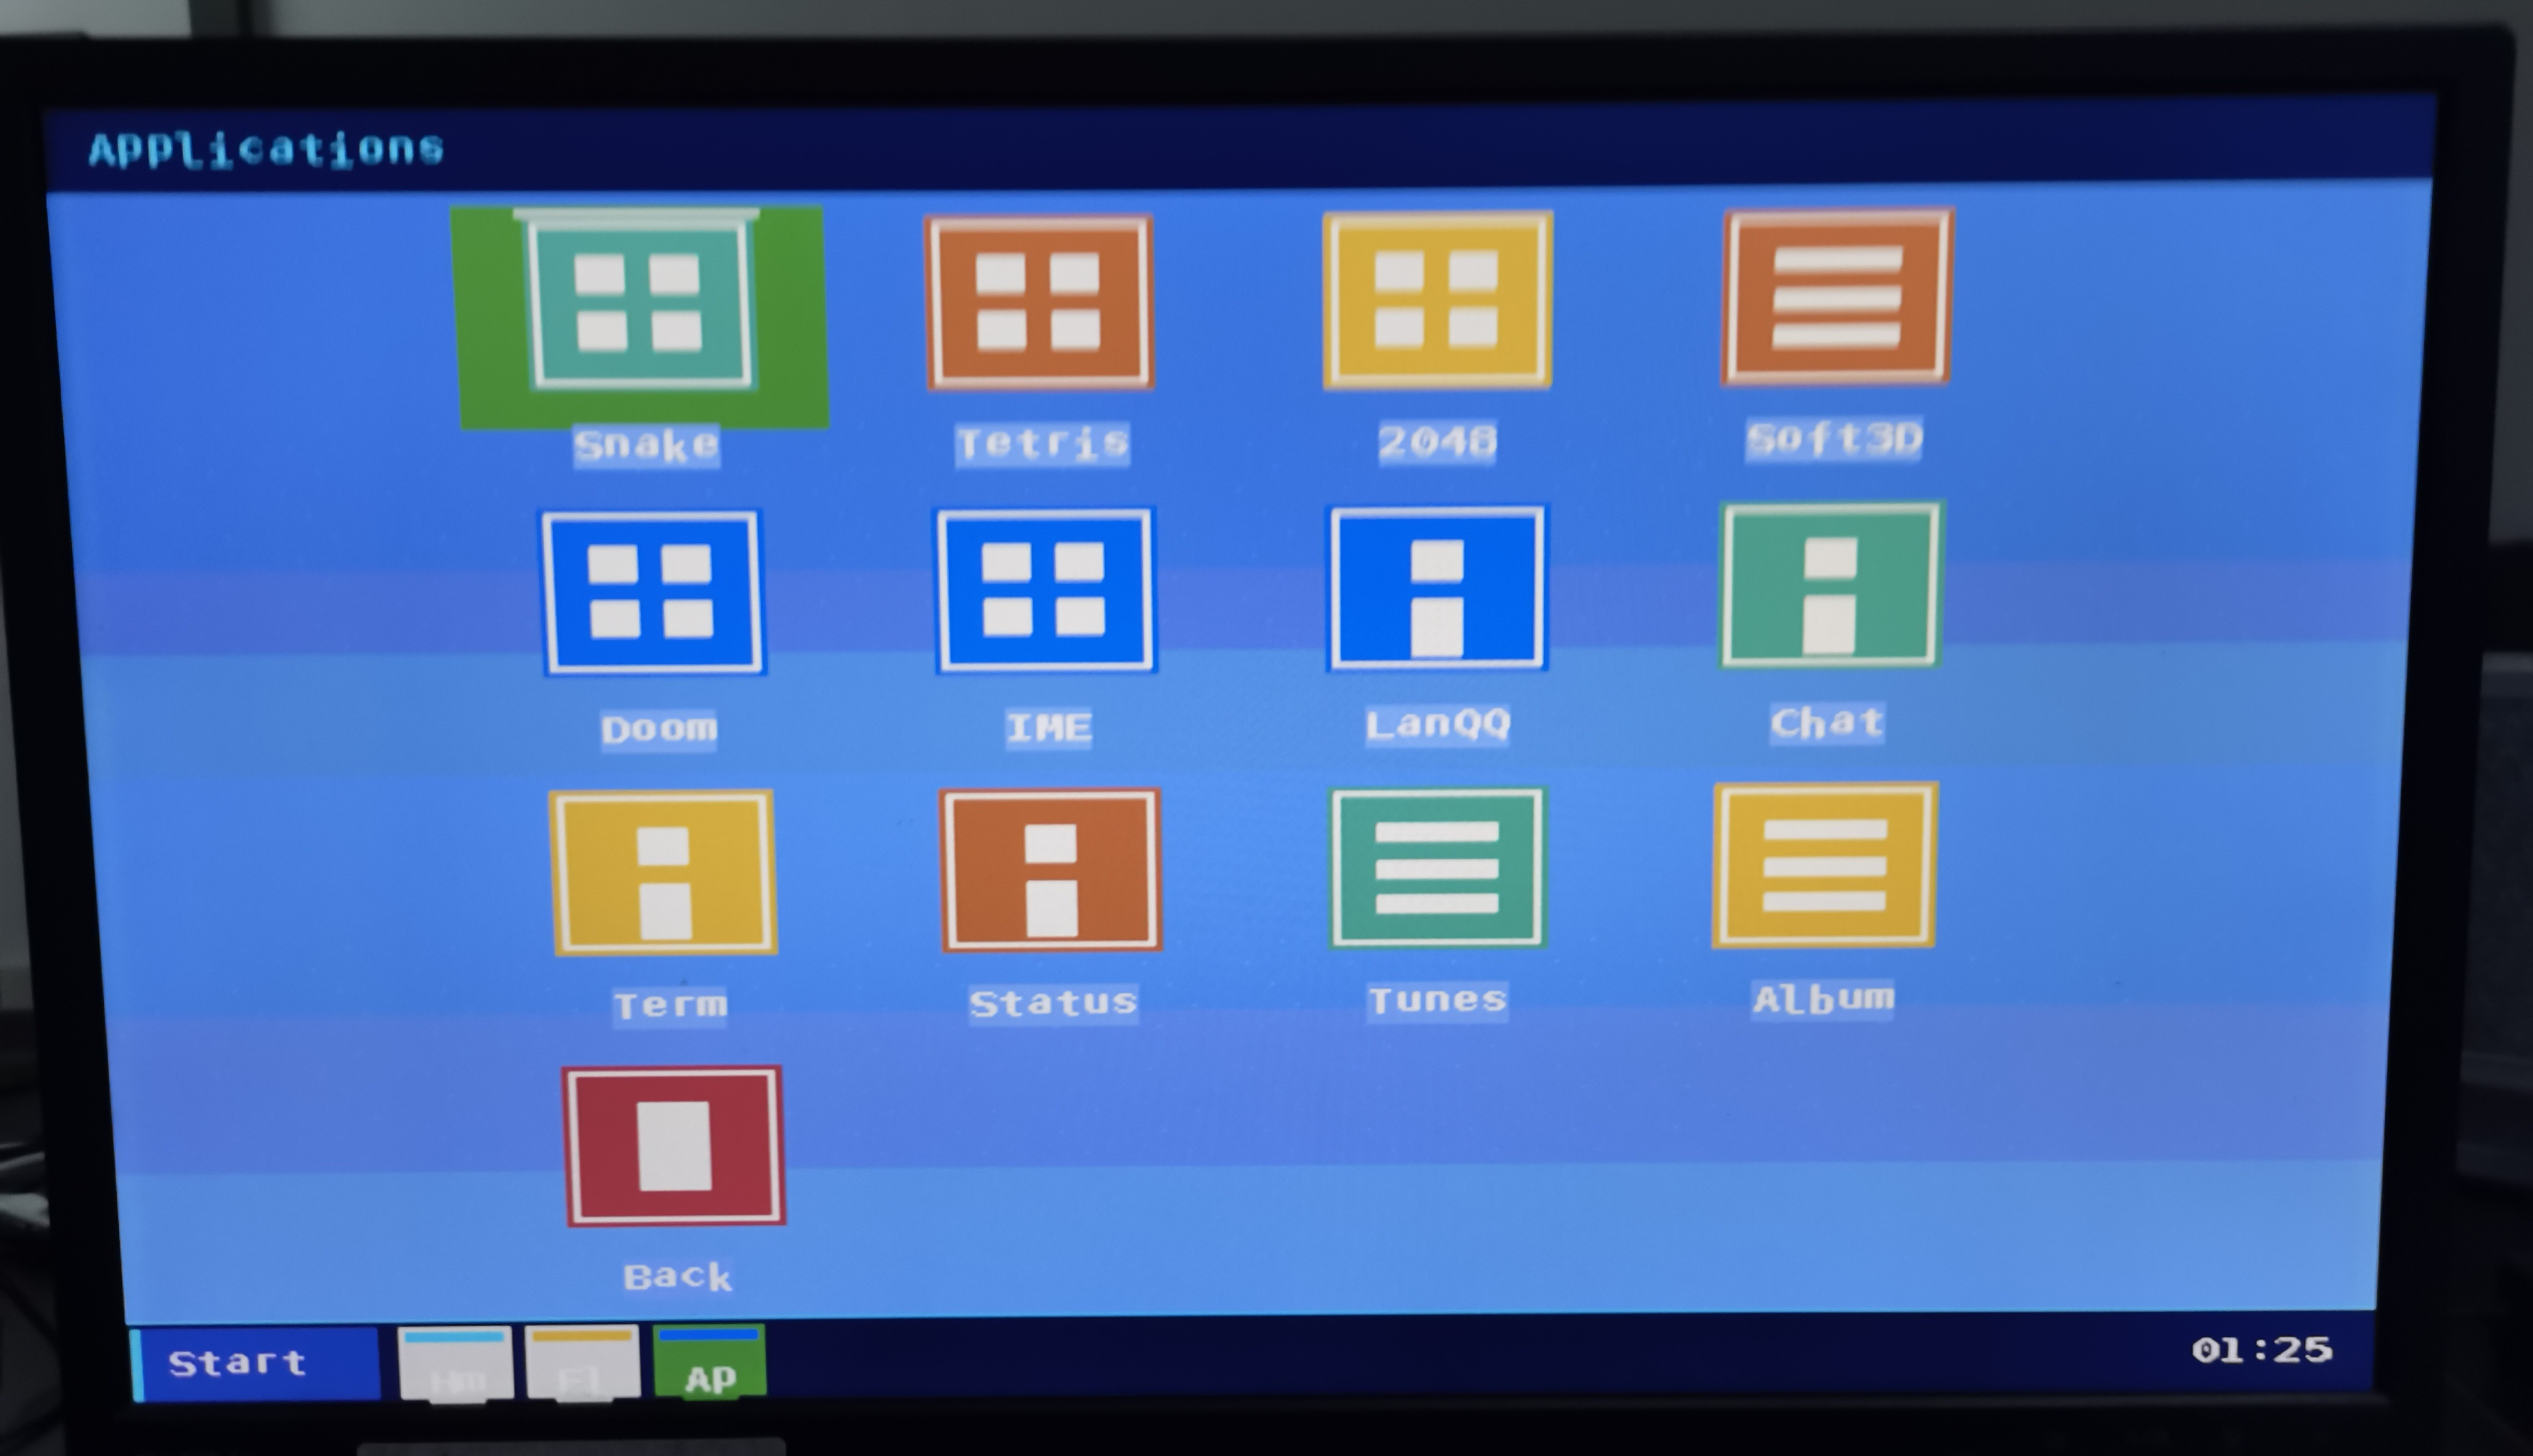
\includegraphics[width=0.95\textwidth]{figure/应用总览.jpg}
  \caption{应用总览}
  \label{fig:应用总览}
\end{figure}

\begin{figure}[H]
  \centering
  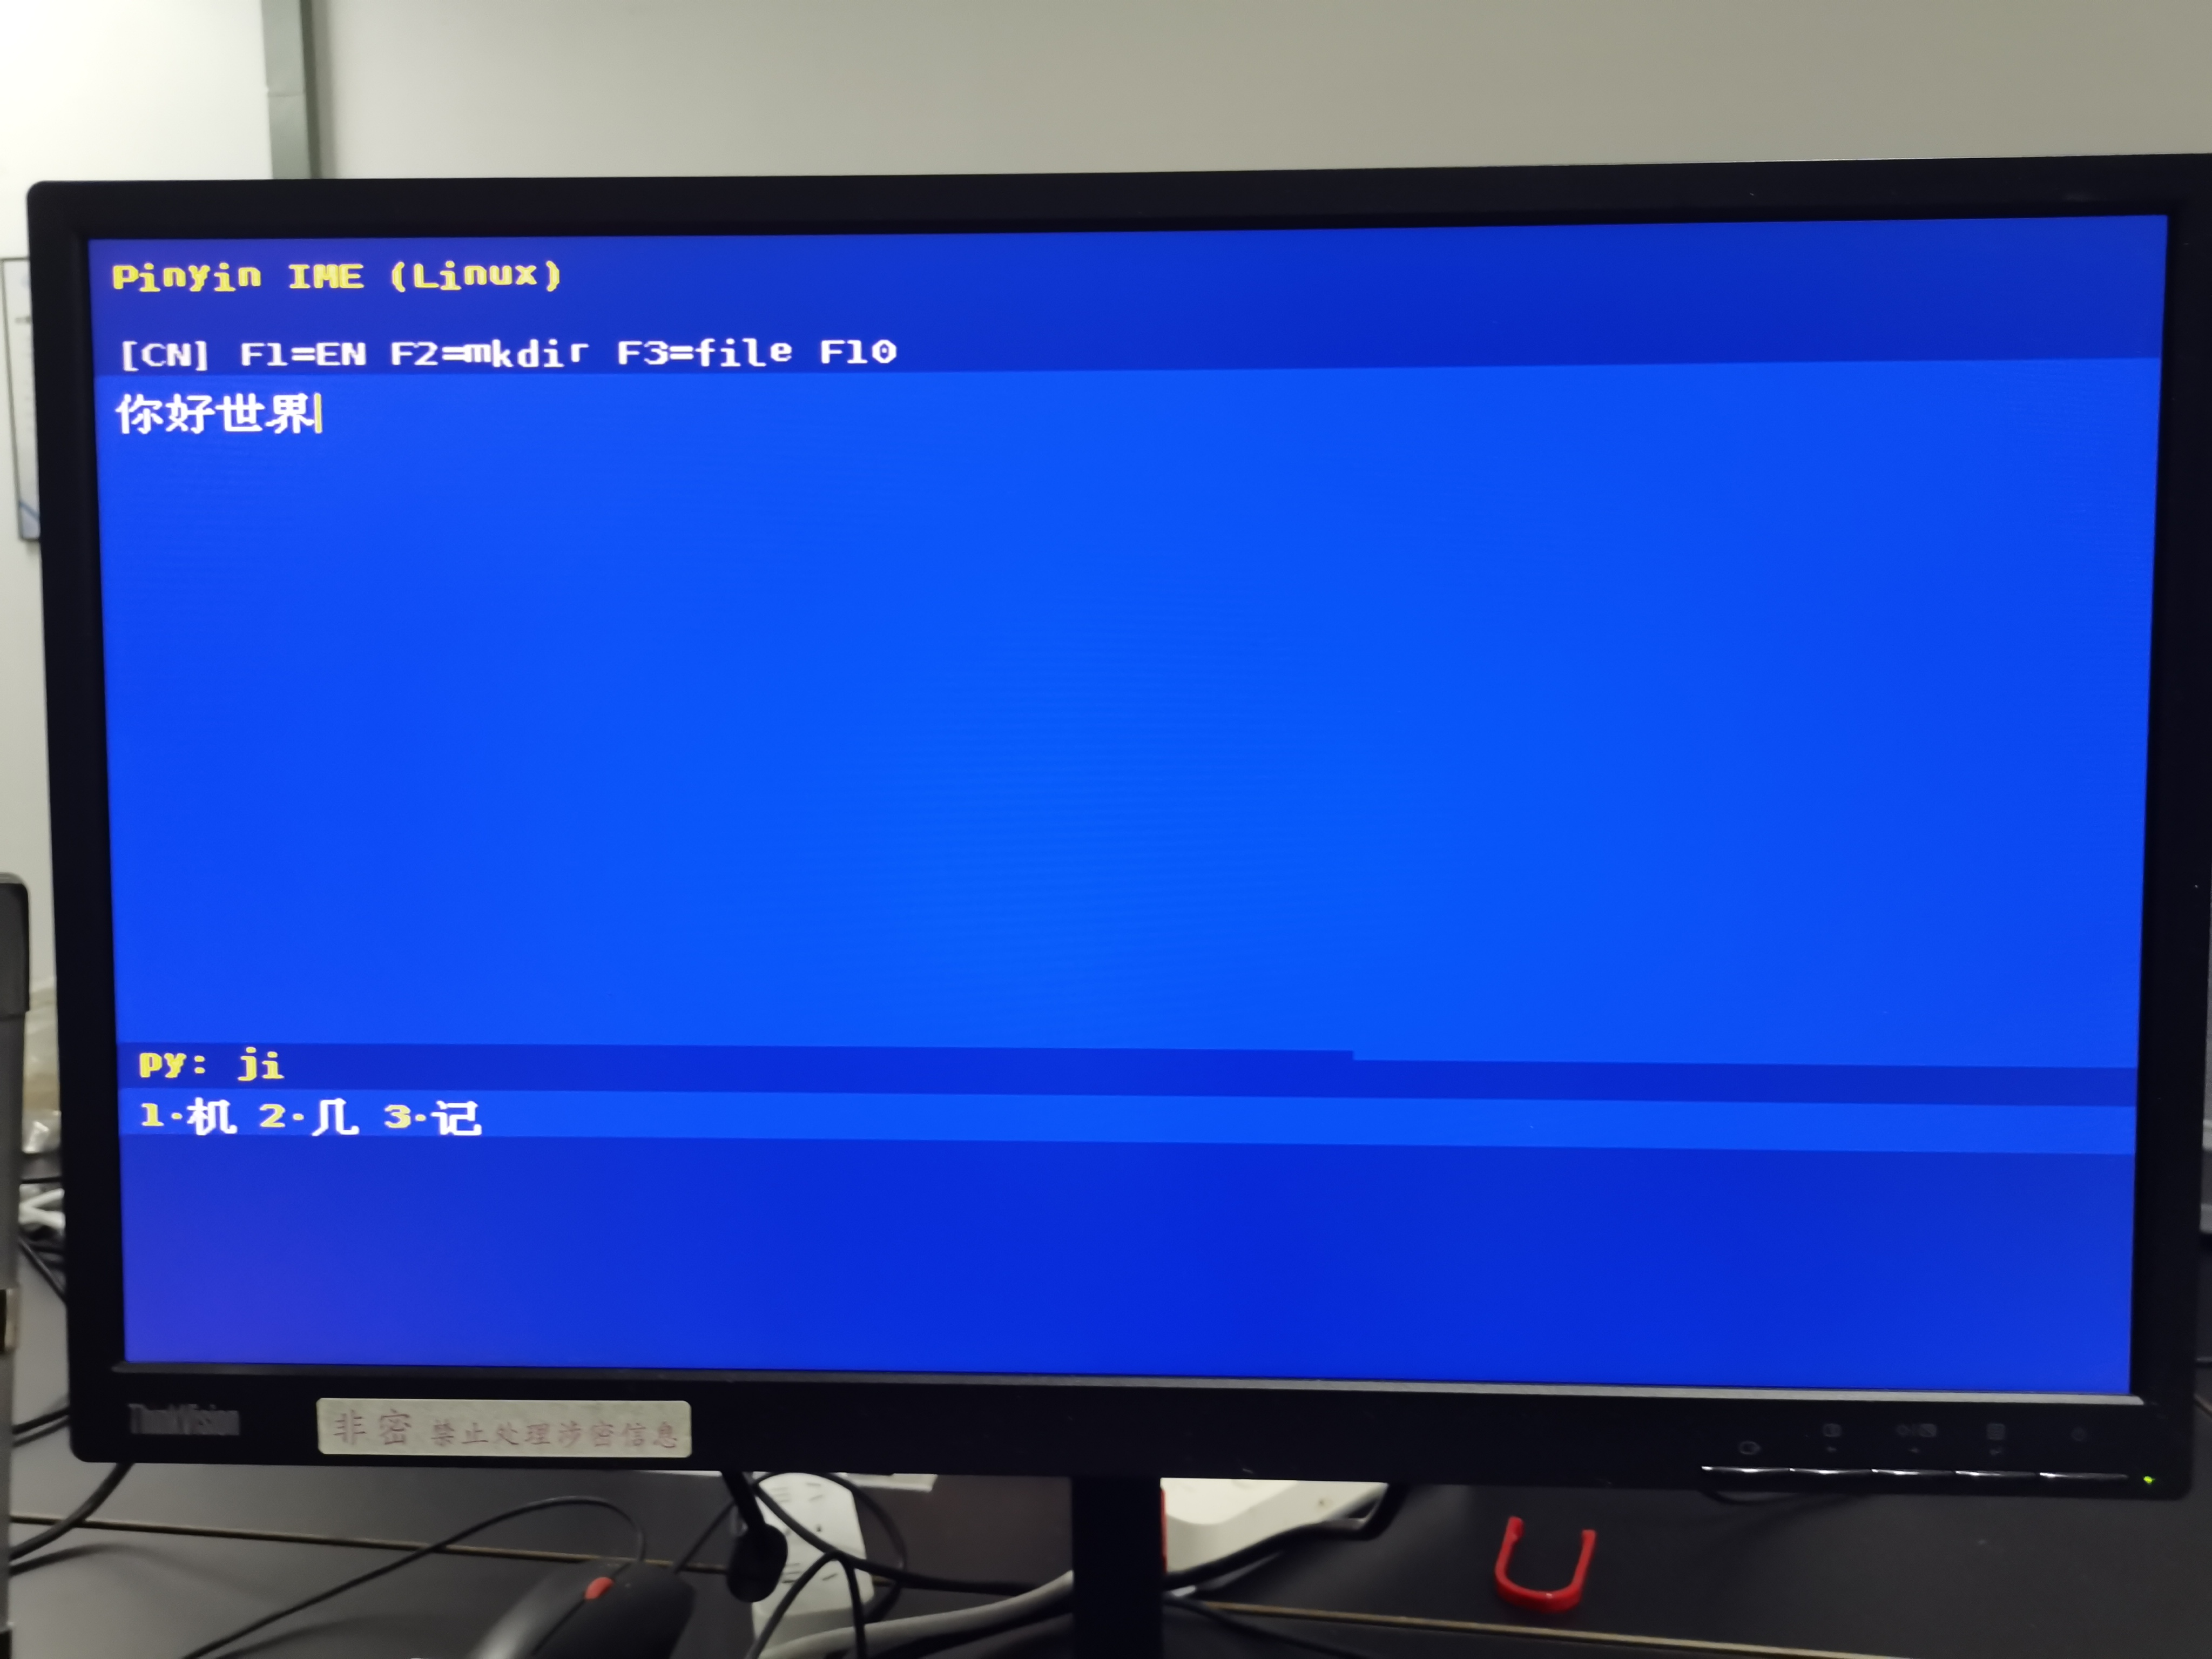
\includegraphics[width=0.95\textwidth]{figure/中文输入法.jpg}
  \caption{中文输入法}
  \label{fig:中文输入法}
\end{figure}

\begin{figure}[H]
  \centering
  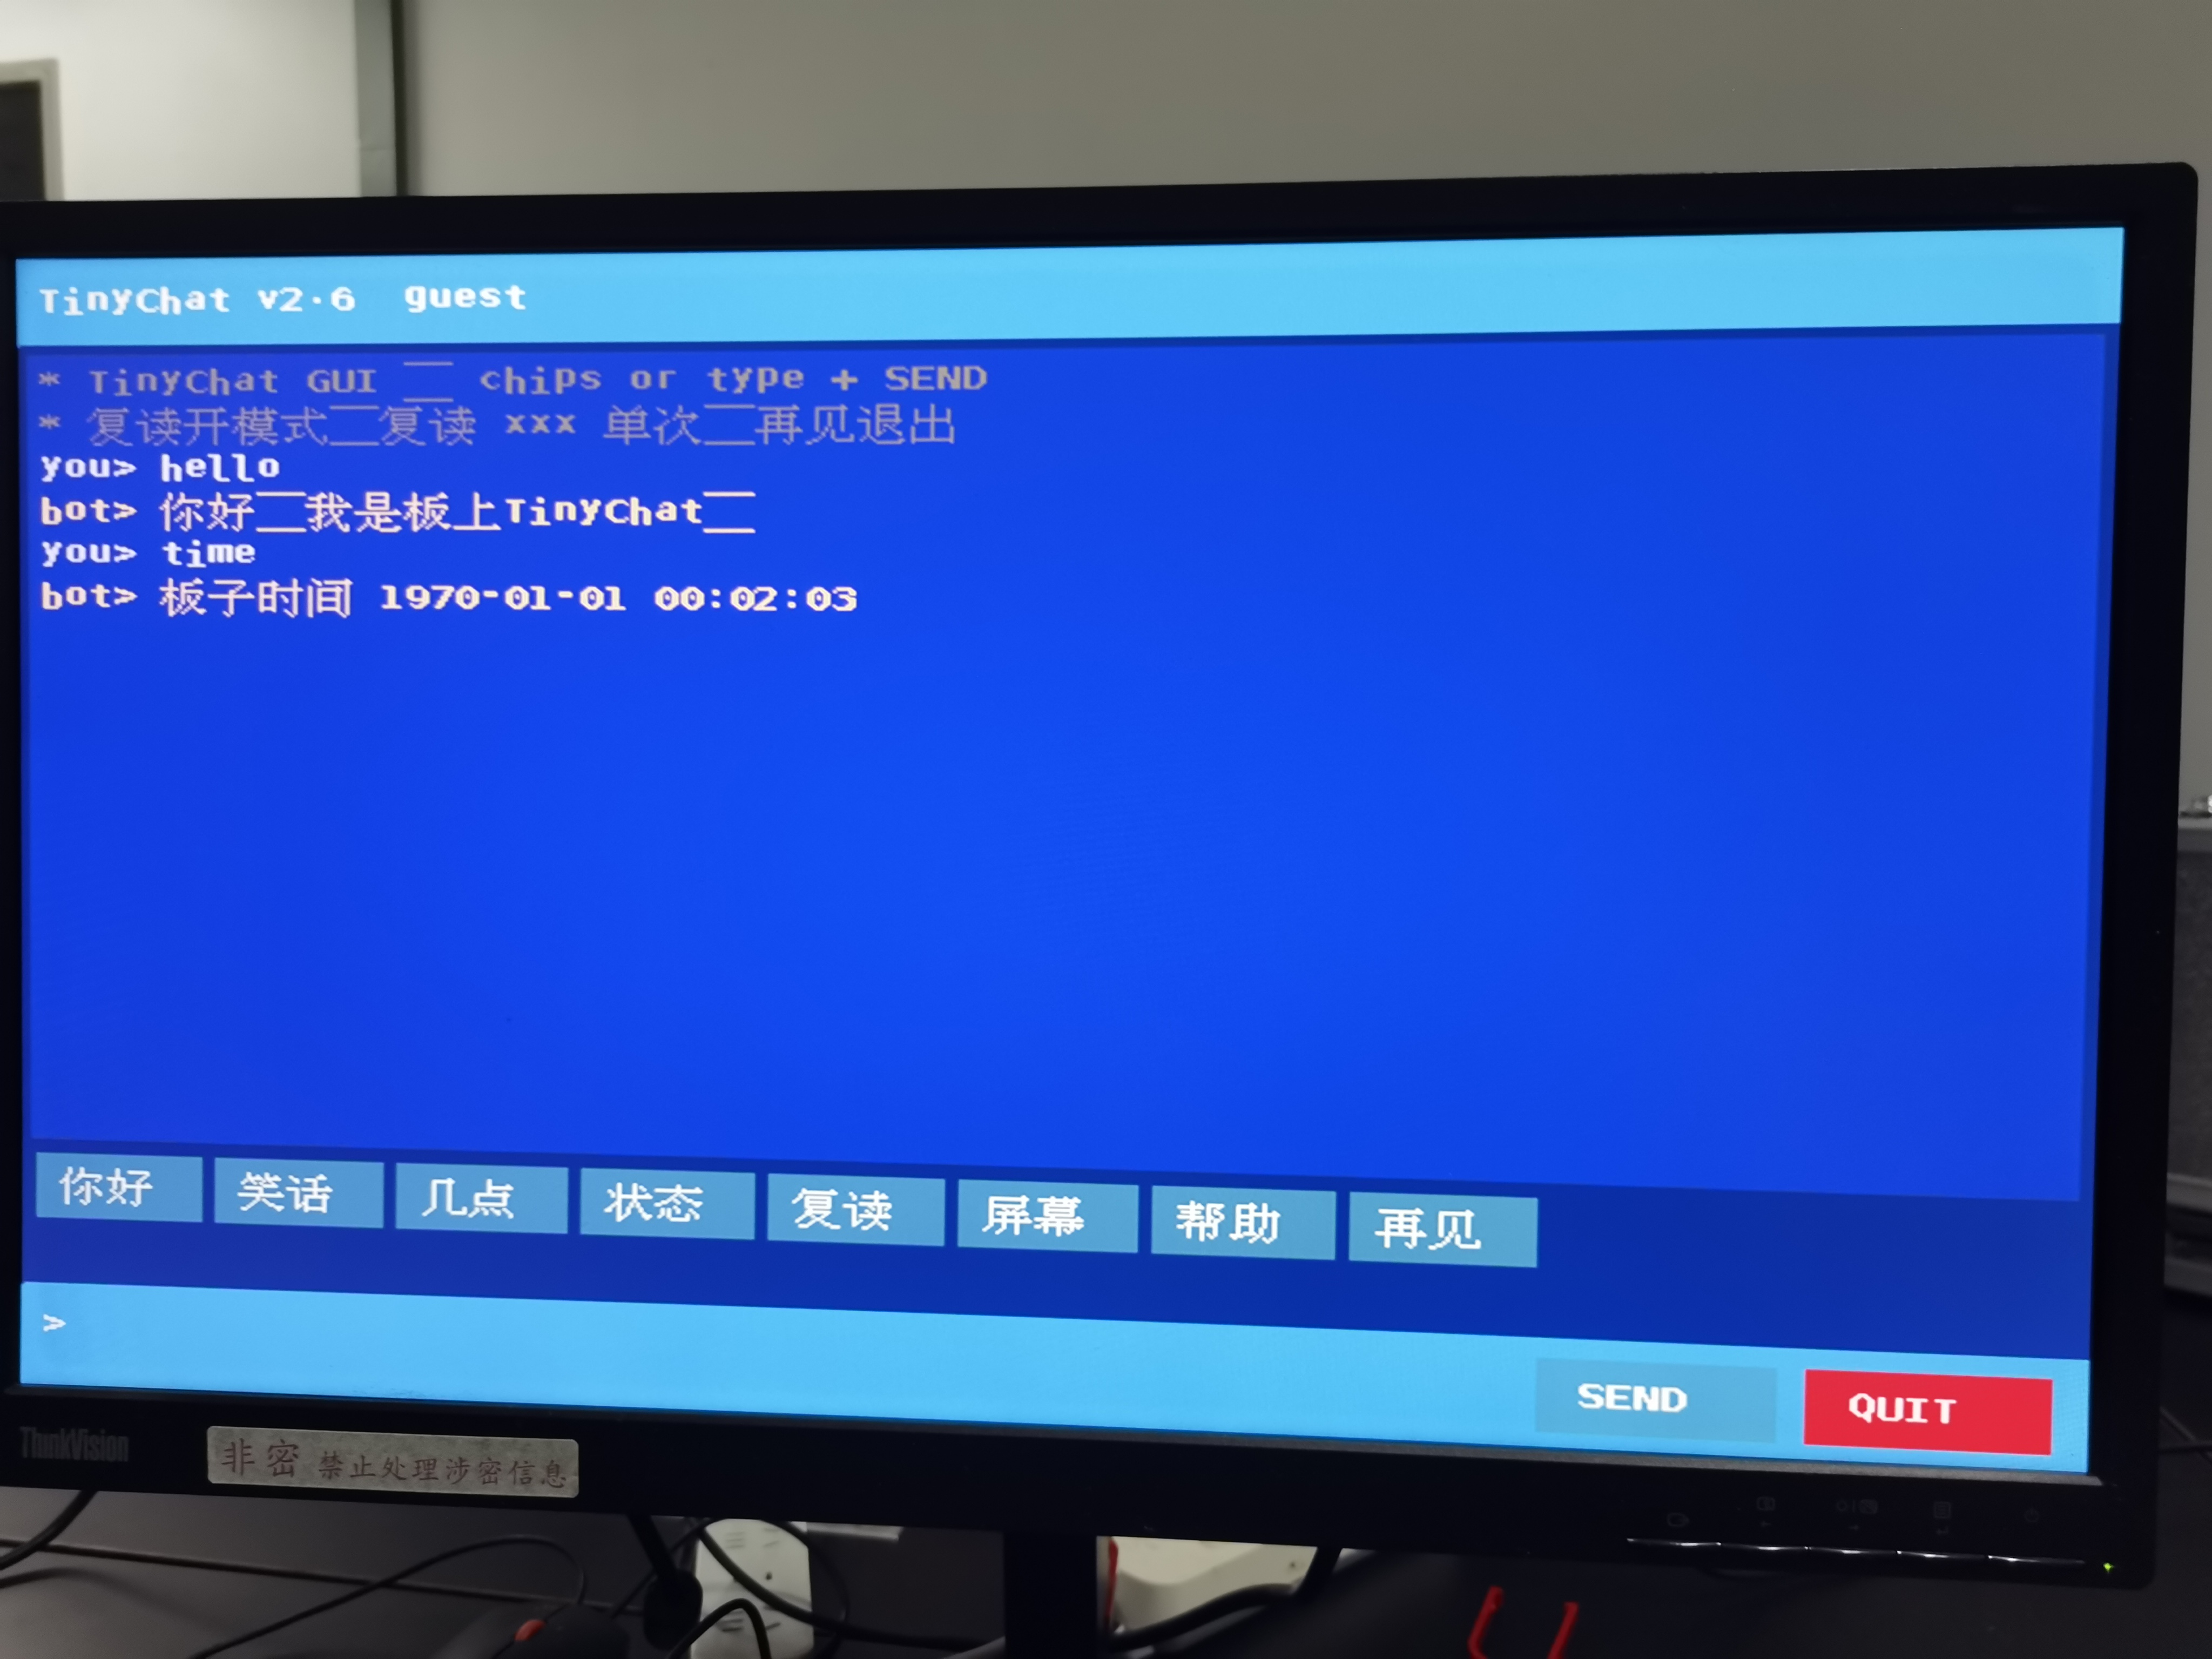
\includegraphics[width=0.95\textwidth]{figure/小AI对话.jpg}
  \caption{小AI对话}
  \label{fig:小AI对话}
\end{figure}

\begin{figure}[H]
  \centering
  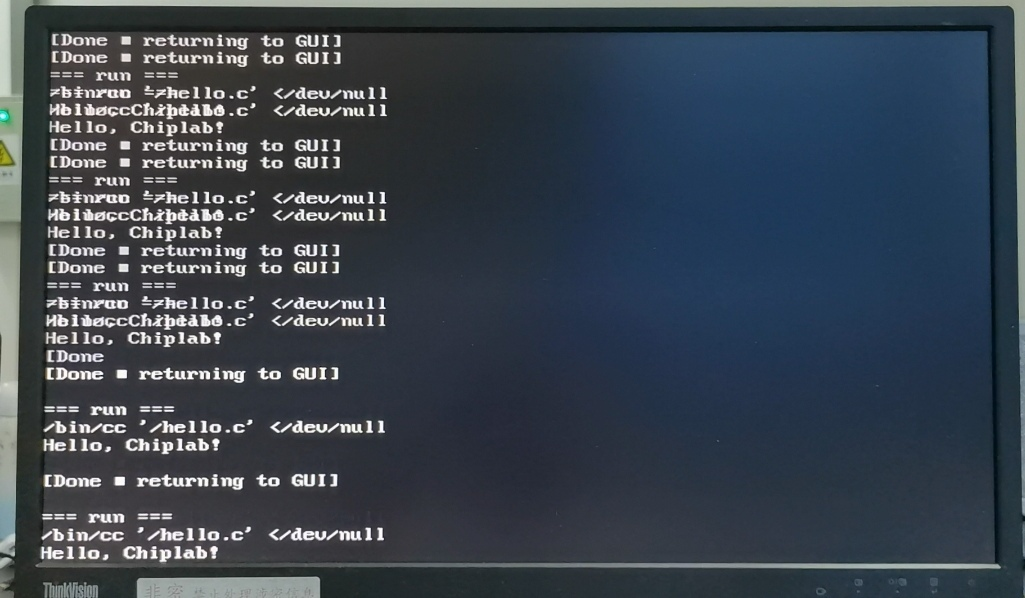
\includegraphics[width=0.95\textwidth]{figure/文件管理系统_执行代码.jpg}
  \caption{执行代码}
  \label{fig:执行代码}
\end{figure}

\begin{figure}[H]
  \centering
  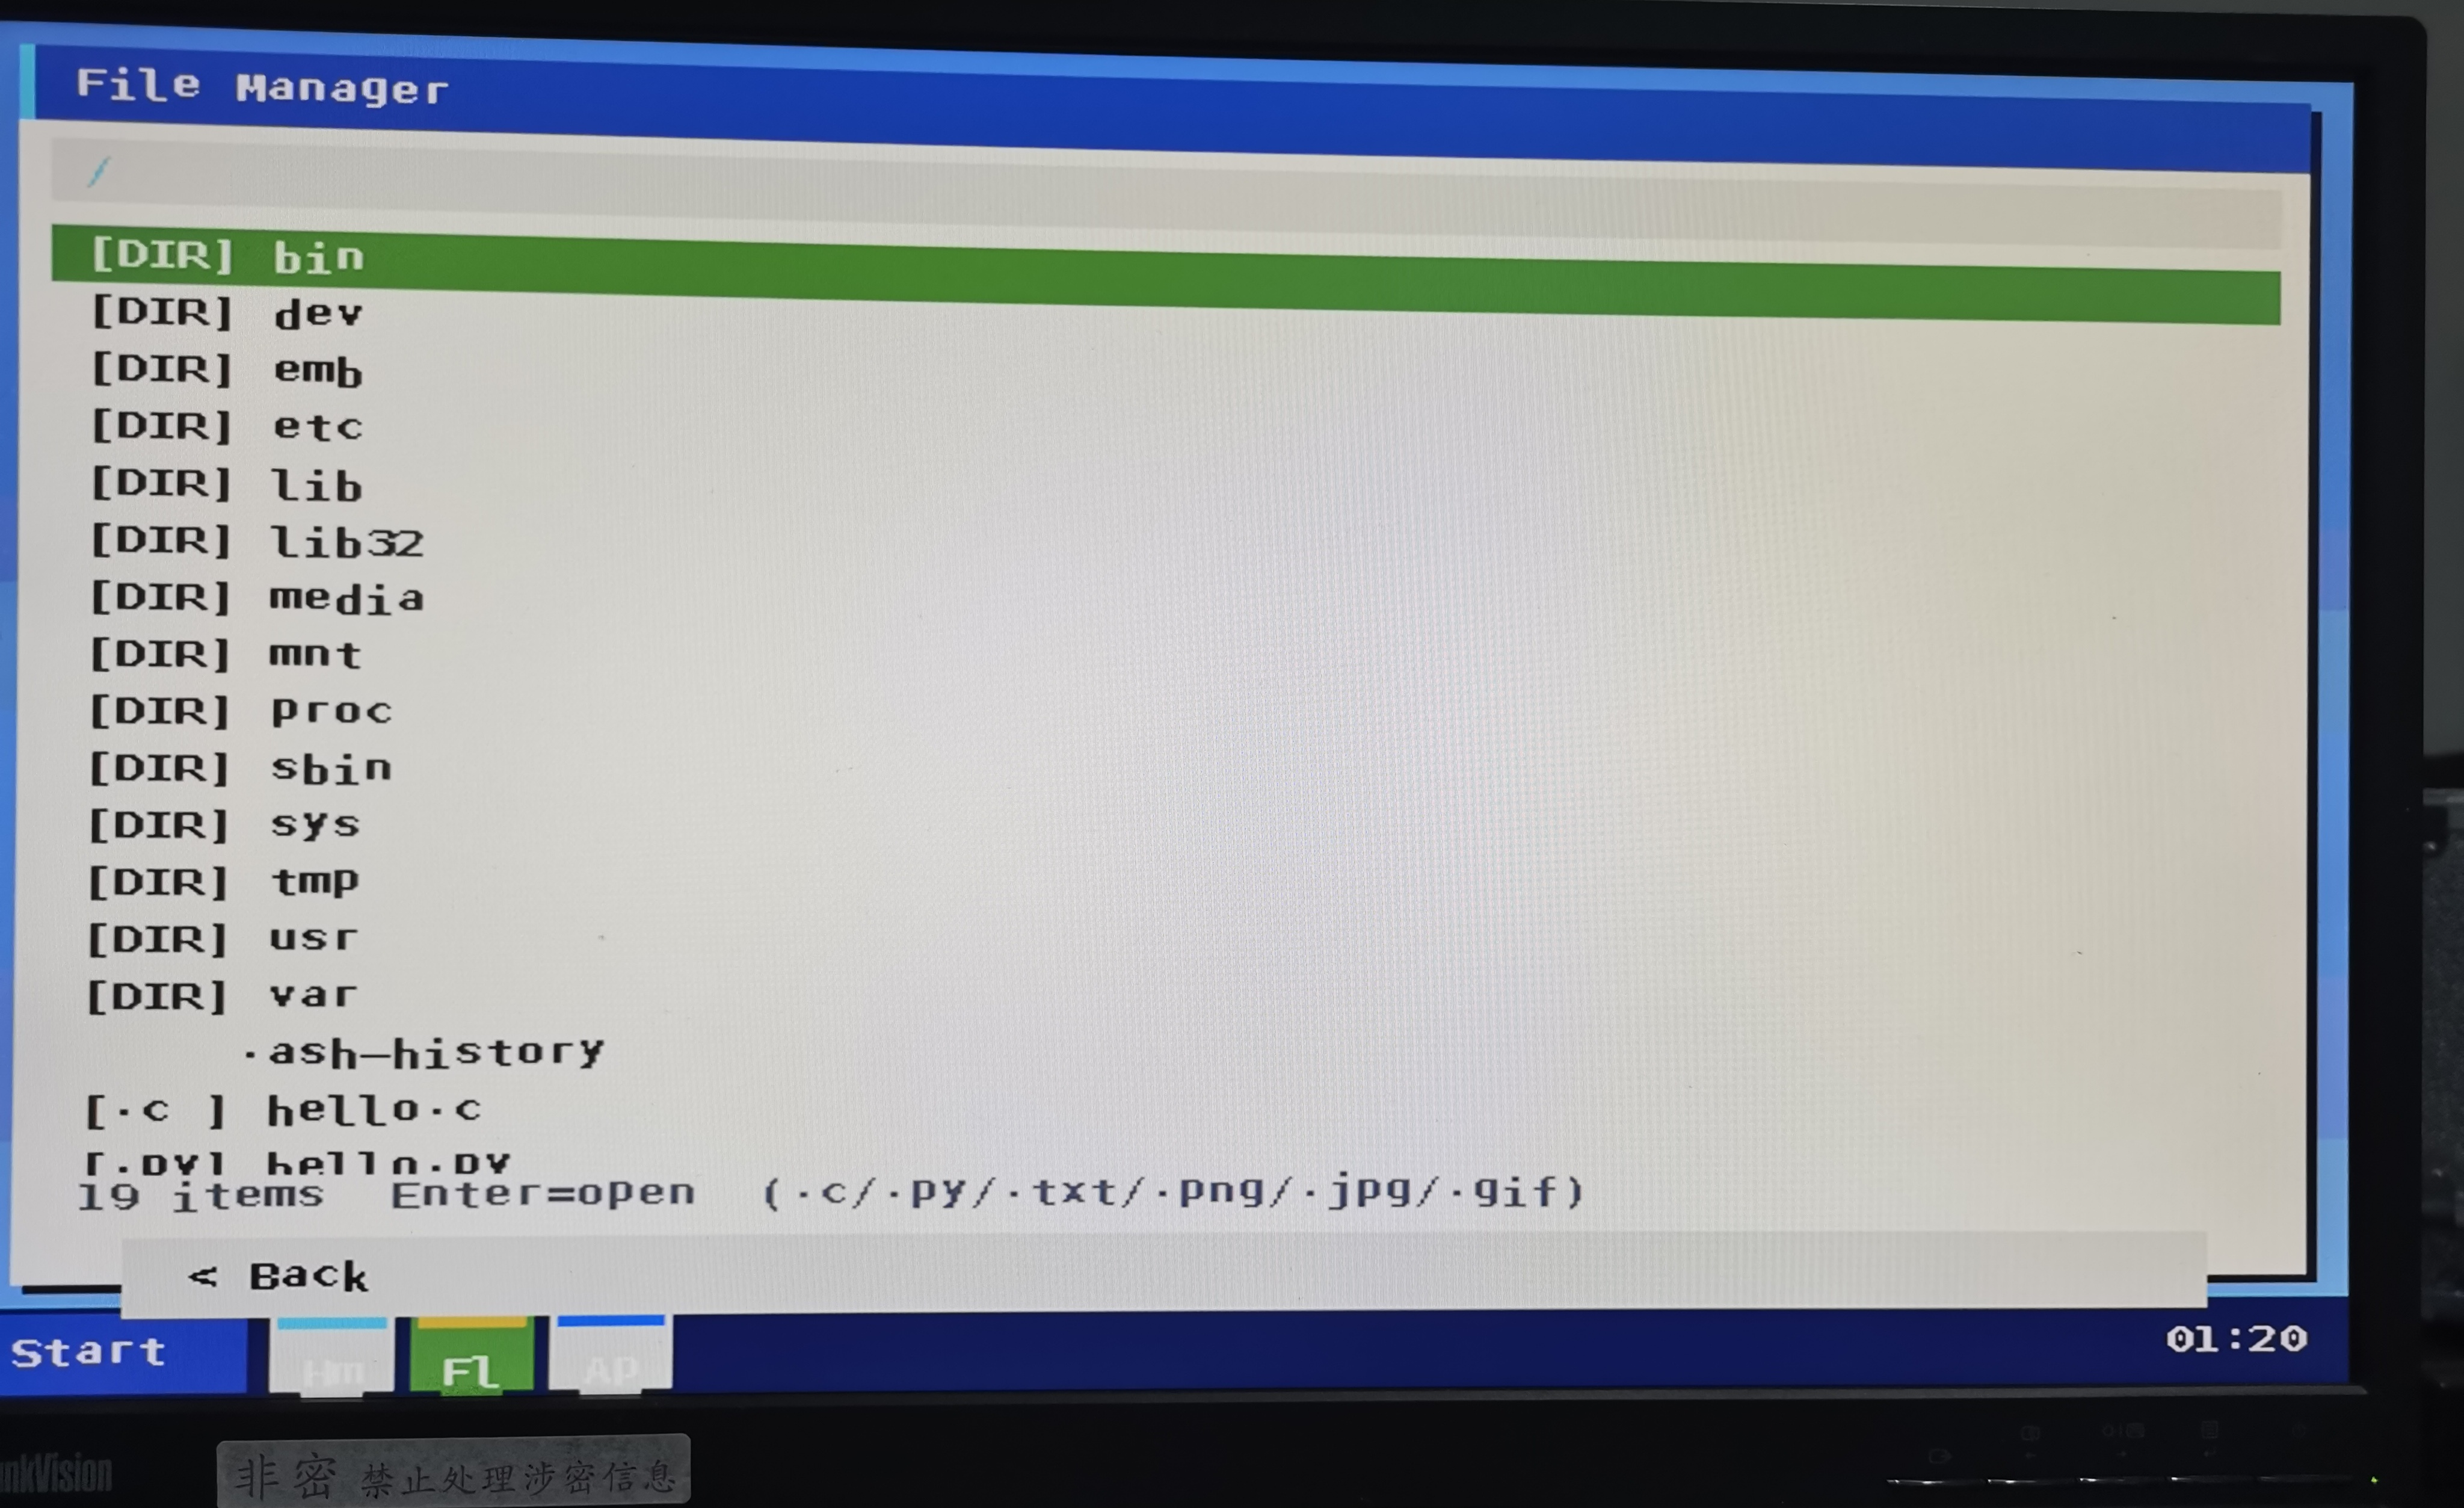
\includegraphics[width=0.95\textwidth]{figure/文件管理系统.jpg}
  \caption{文件管理系统}
  \label{fig:文件管理系统}
\end{figure}

\begin{figure}[H]
  \centering
  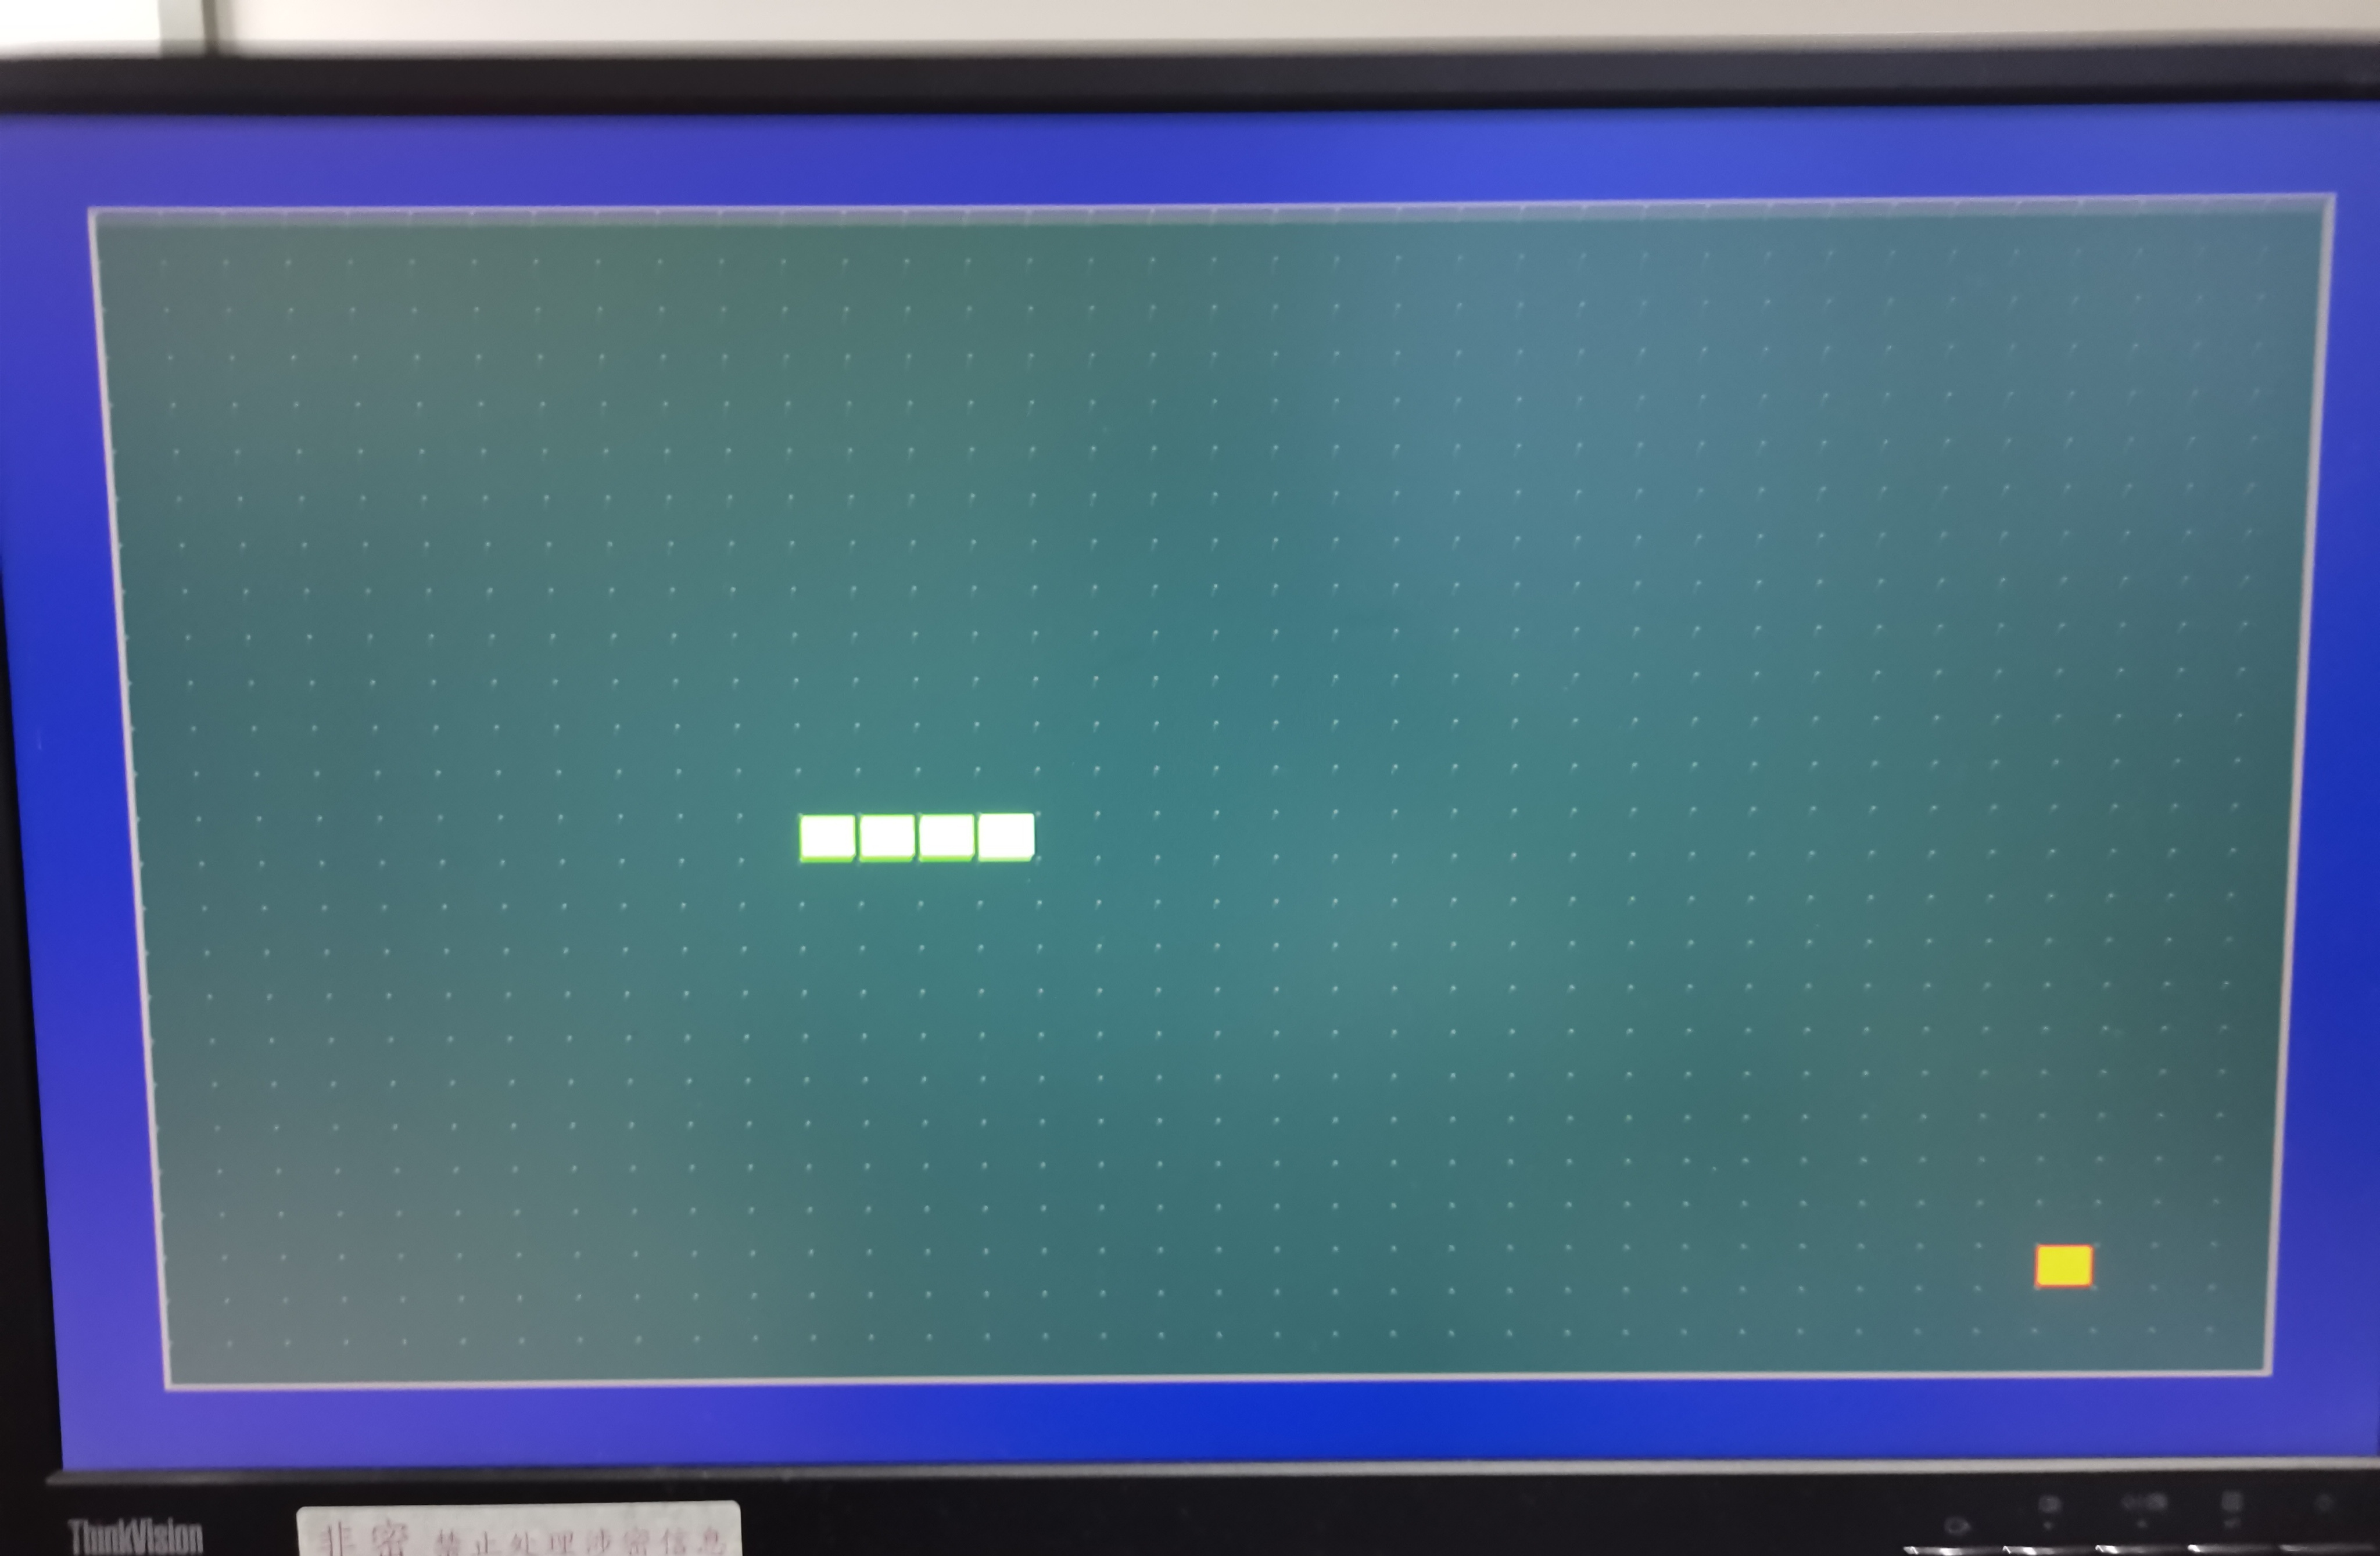
\includegraphics[width=0.95\textwidth]{figure/贪吃蛇.jpg}
  \caption{贪吃蛇}
  \label{fig:贪吃蛇}
\end{figure}

\begin{figure}[H]
  \centering
  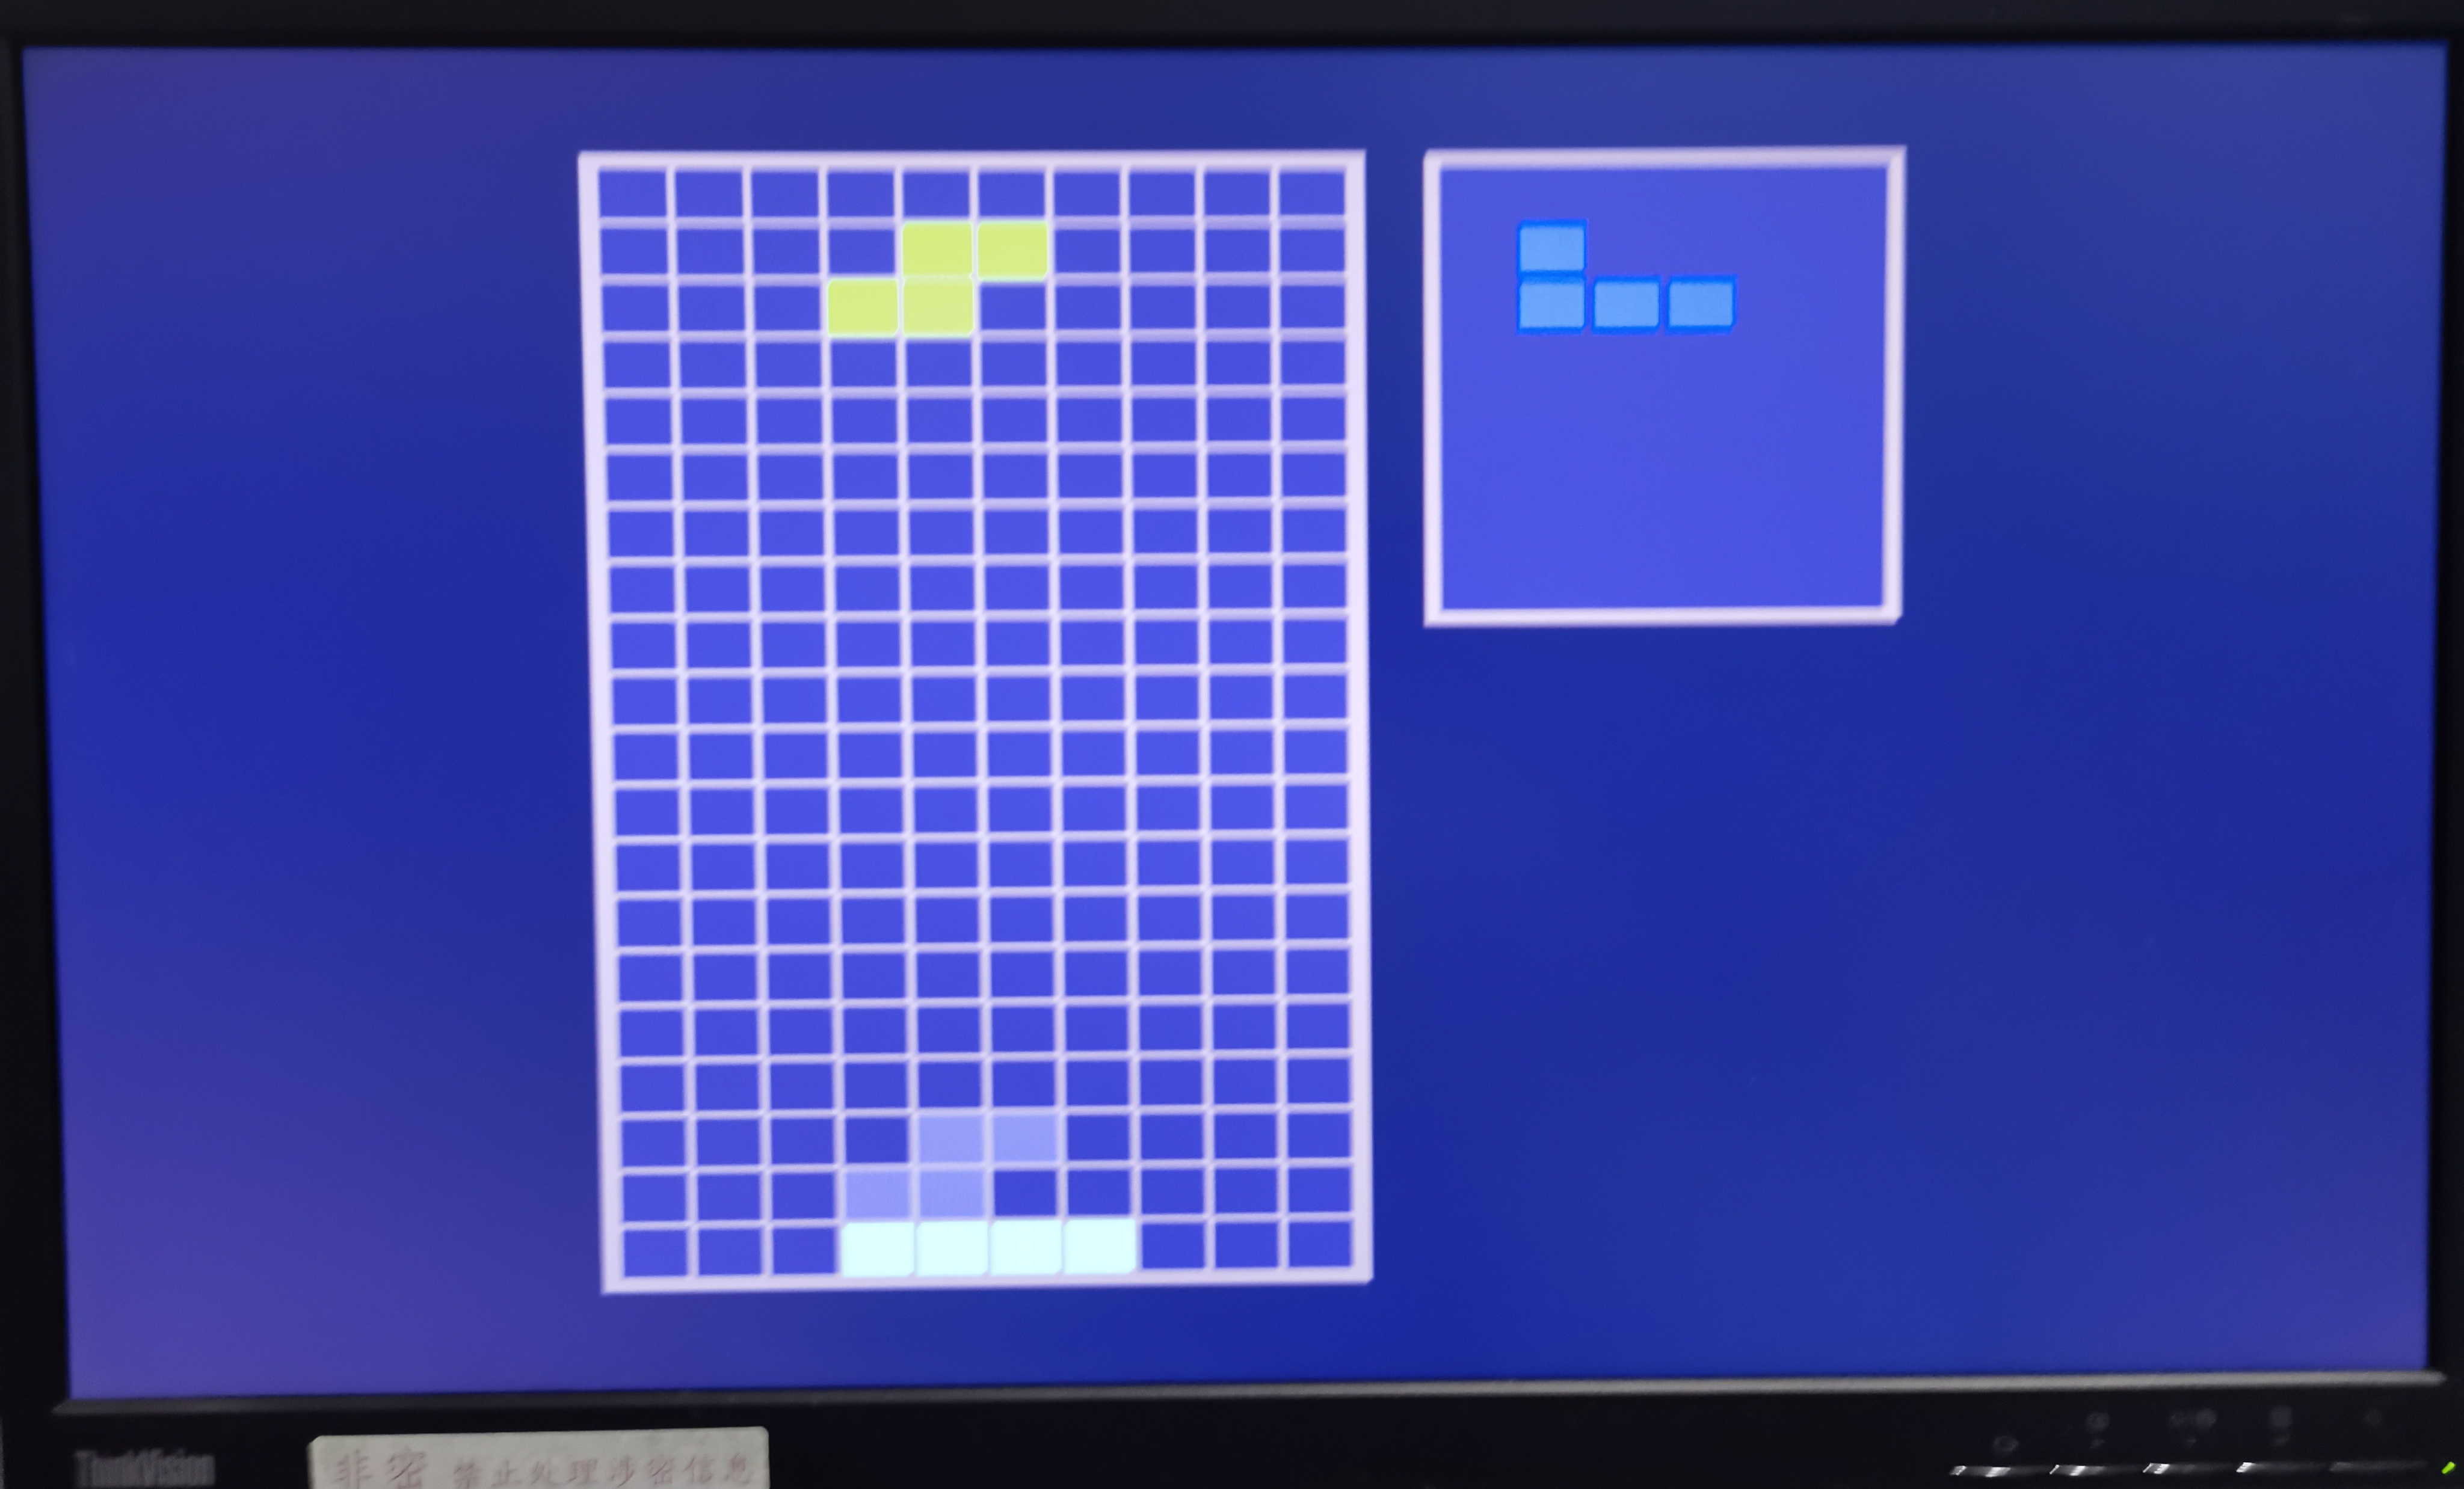
\includegraphics[width=0.95\textwidth]{figure/俄罗斯方块.jpg}
  \caption{俄罗斯方块}
  \label{fig:俄罗斯方块}
\end{figure}

\begin{figure}[H]
  \centering
  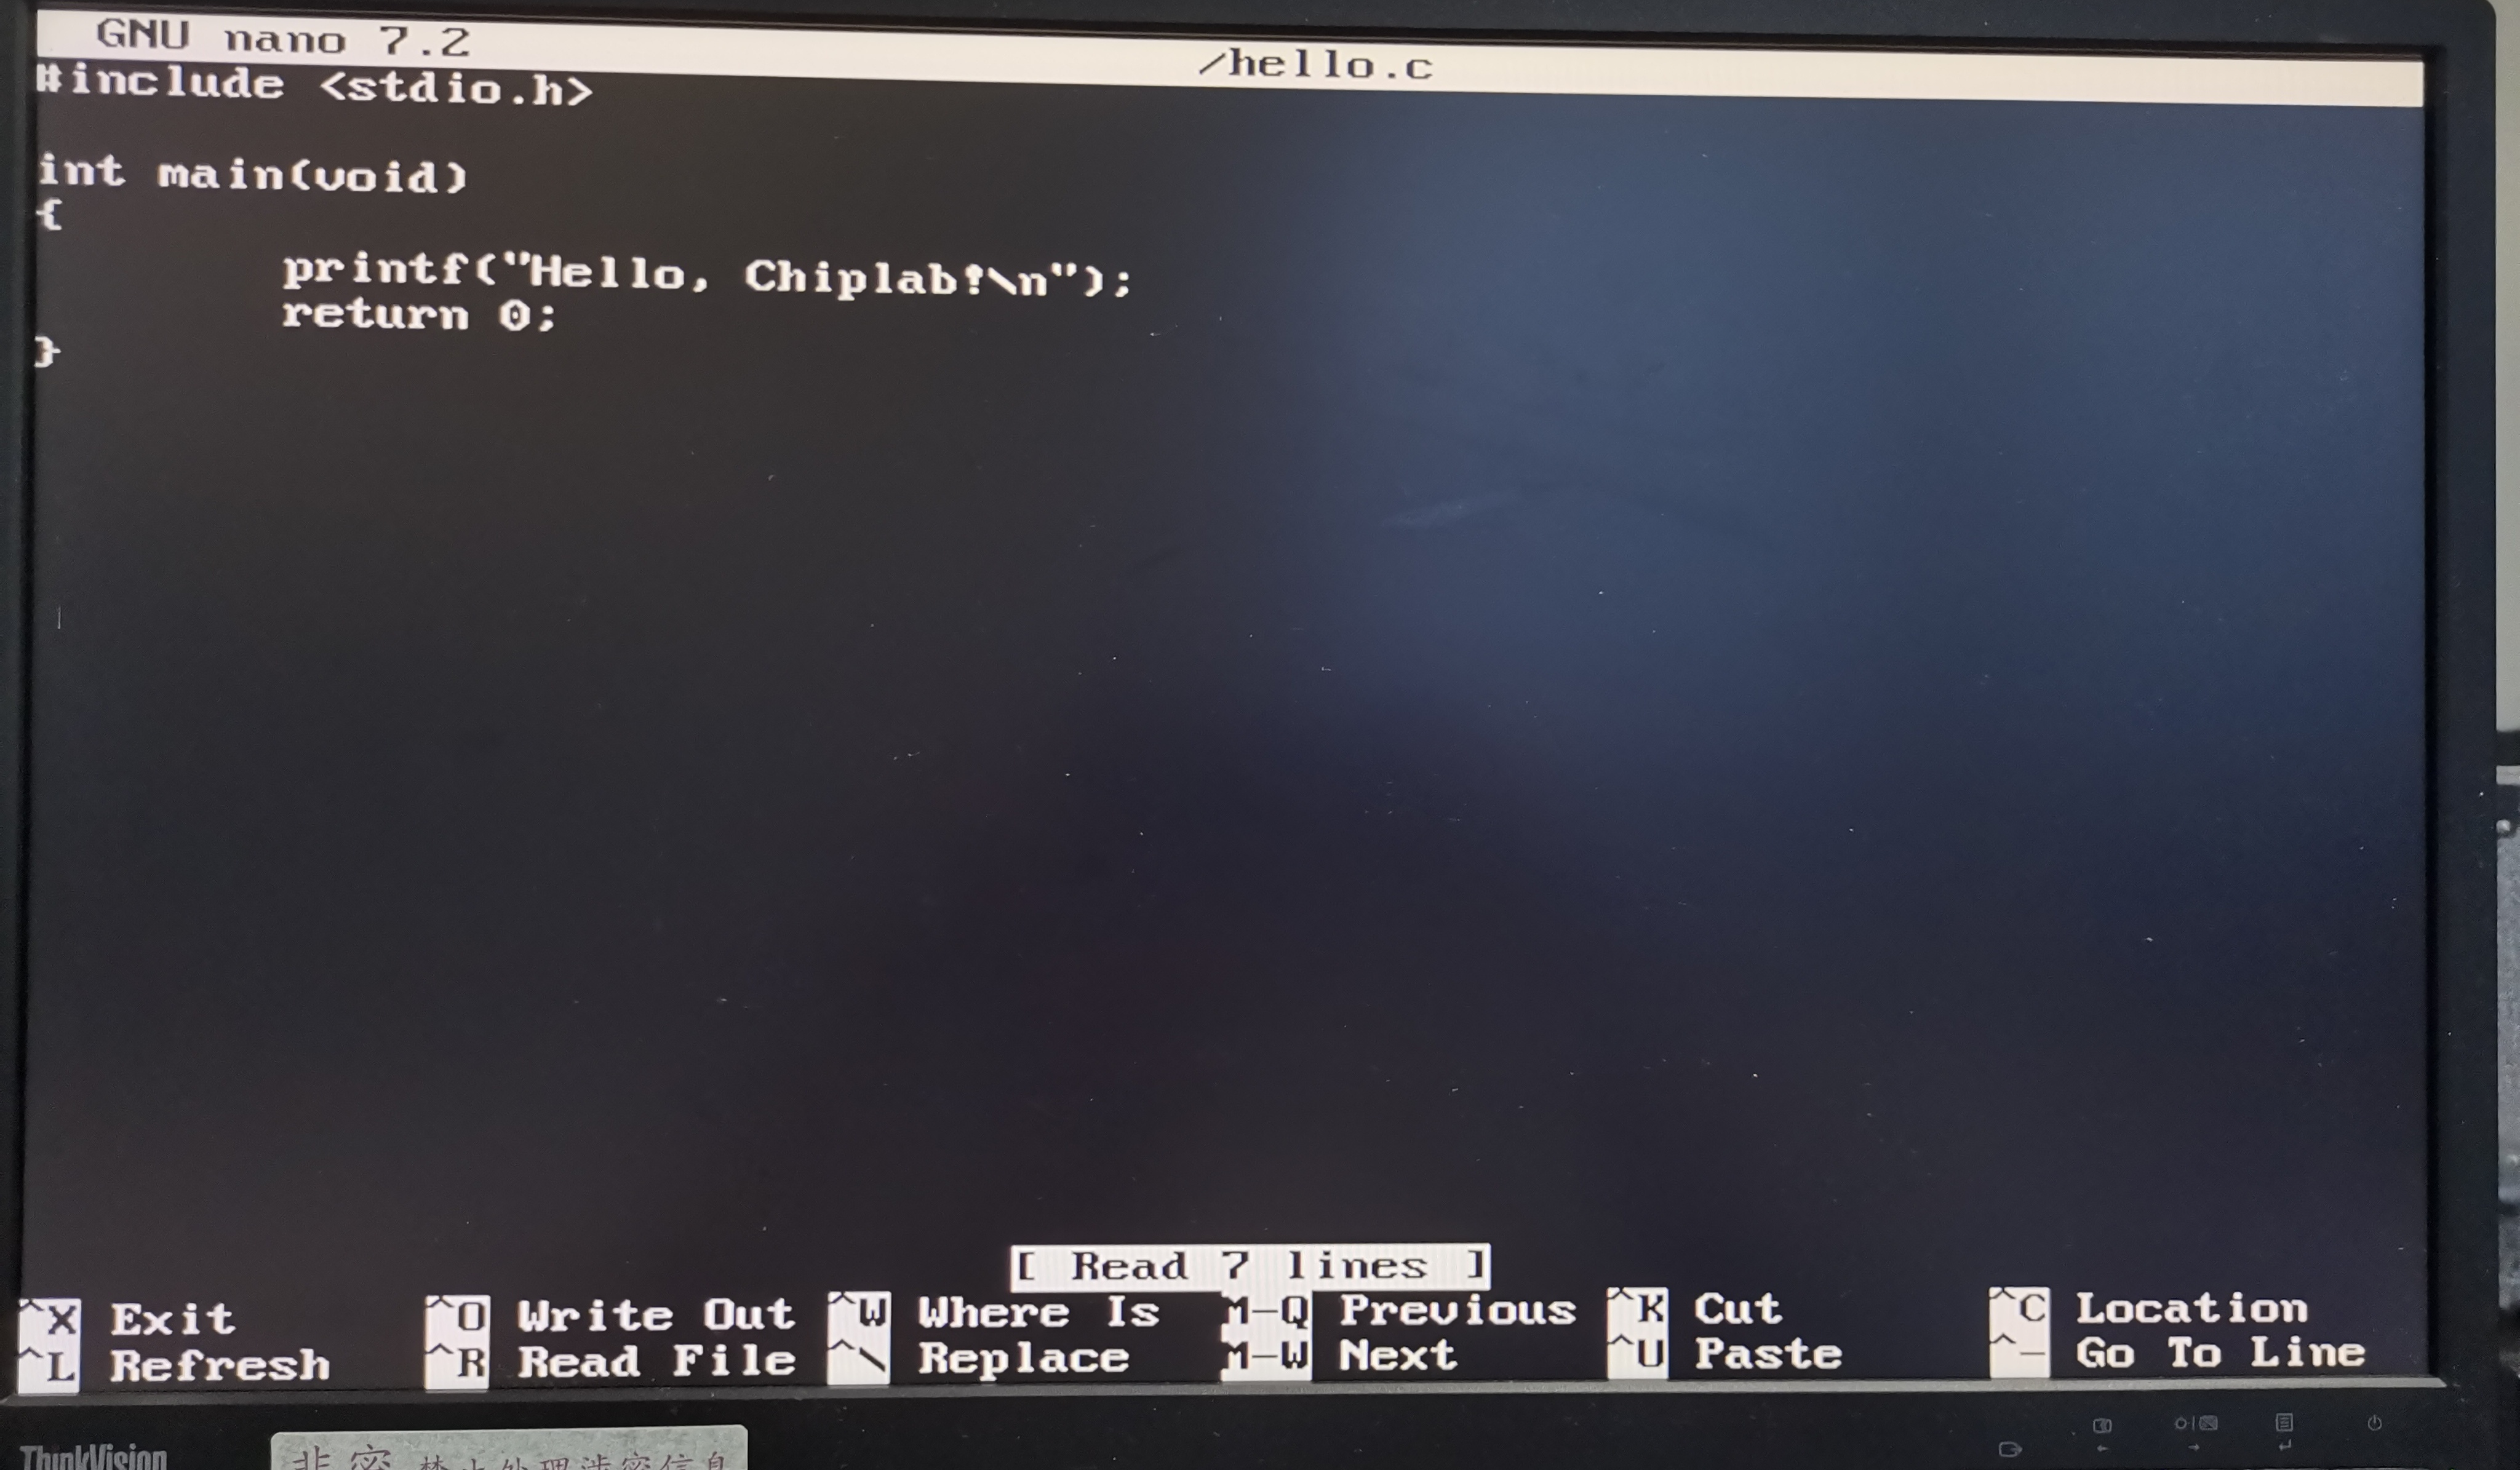
\includegraphics[width=0.95\textwidth]{figure/NANO.jpg}
  \caption{NANO}
  \label{fig:NANO}
\end{figure}

\begin{figure}[H]
  \centering
  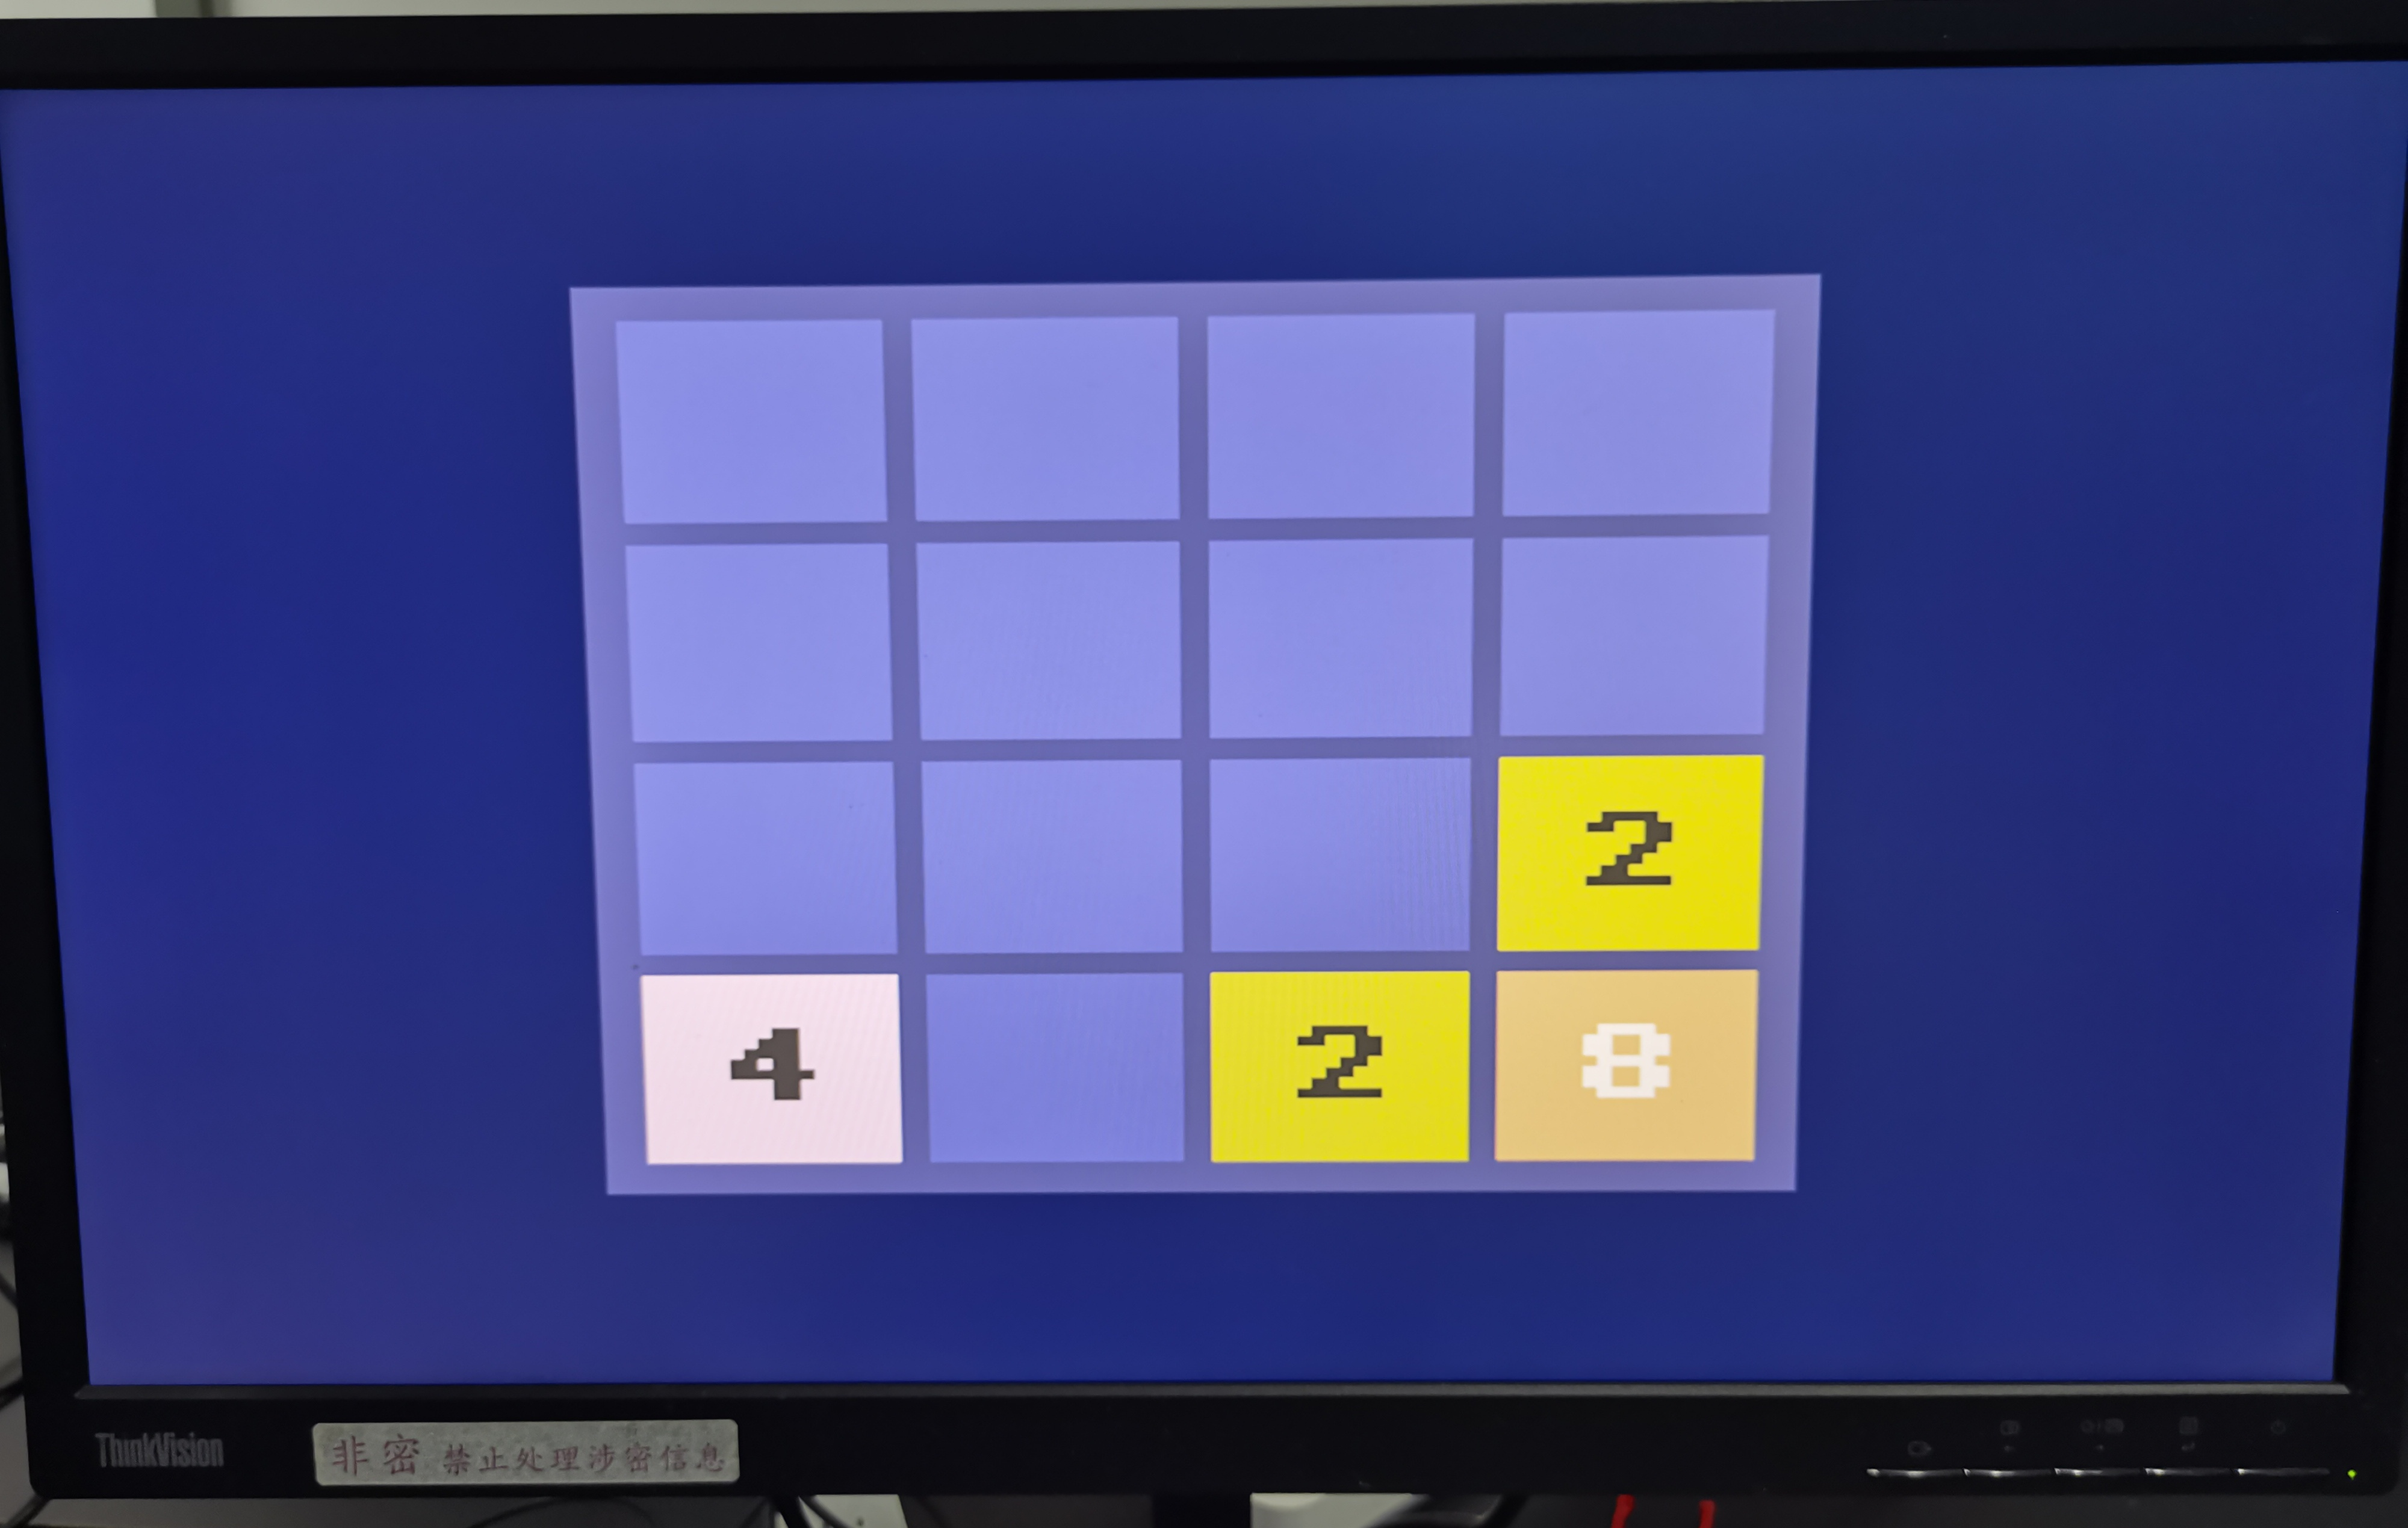
\includegraphics[width=0.95\textwidth]{figure/2048.jpg}
  \caption{2048}
  \label{fig:2048}
\end{figure}

\begin{figure}[H]
  \centering
  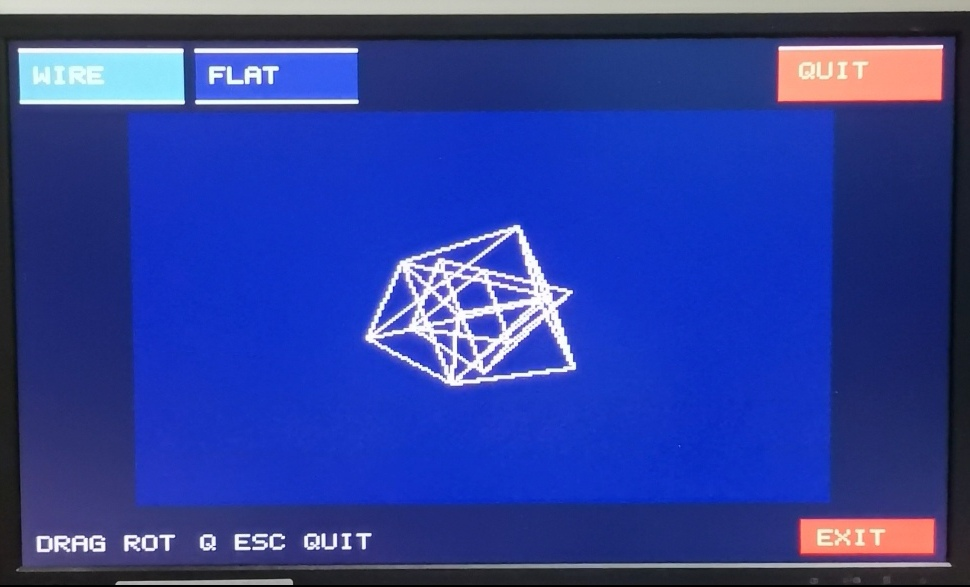
\includegraphics[width=0.95\textwidth]{figure/3D渲染_线条.jpg}
  \caption{3D渲染}
  \label{fig:3D渲染}
\end{figure}















\section{设计结果}

\subsection{设计交付物}

\begin{verbatim}
|- score.xlsx              Excel：功能/性能测试得分
|- design.pdf              PDF：设计文档
|- .gitlab-ci.yml          CI/CD 配置
|-- src/
|    |-- mycpu/            我们的 CPU 完整源码
|    |    |-- xilinx_ip/   我们的 CPU 没有使用 IP 核 
|    |-- vivado_cannot/    无
|    |-- perf_clock.json   性能测试 CPU 主频
|-- bit/                   各项测试生成的 bit 文件
|-- show/                  决赛展示内容
\end{verbatim}

\subsection{CPU 功能与性能结果}

\begin{table}[H]
\centering
\caption{CPU 功能与性能测试结果}
\label{tab:perf}
\small
\begin{tabularx}{\textwidth}{>{\raggedright\arraybackslash}p{4.0cm}>{\raggedright\arraybackslash}p{4.0cm}X}
\toprule
项目 & 结果 & 说明 \\
\midrule
功能分 & \textbf{100.000000} & 58/58 点；最差 seed 通过，3/3 seed 通过 \\
IPC 比值 & \textbf{1.934633120} & IPC ratio \\
系统计数器比值 & \textbf{4.438258572} & system count ratio \\
最高实现频率 & \textbf{75.001875\,MHz} & \texttt{cpu\_clk} WNS $+0.052$\,ns \\
\bottomrule
\end{tabularx}
\end{table}

\subsection{linux启动}

\begin{figure}[H]
  \centering
  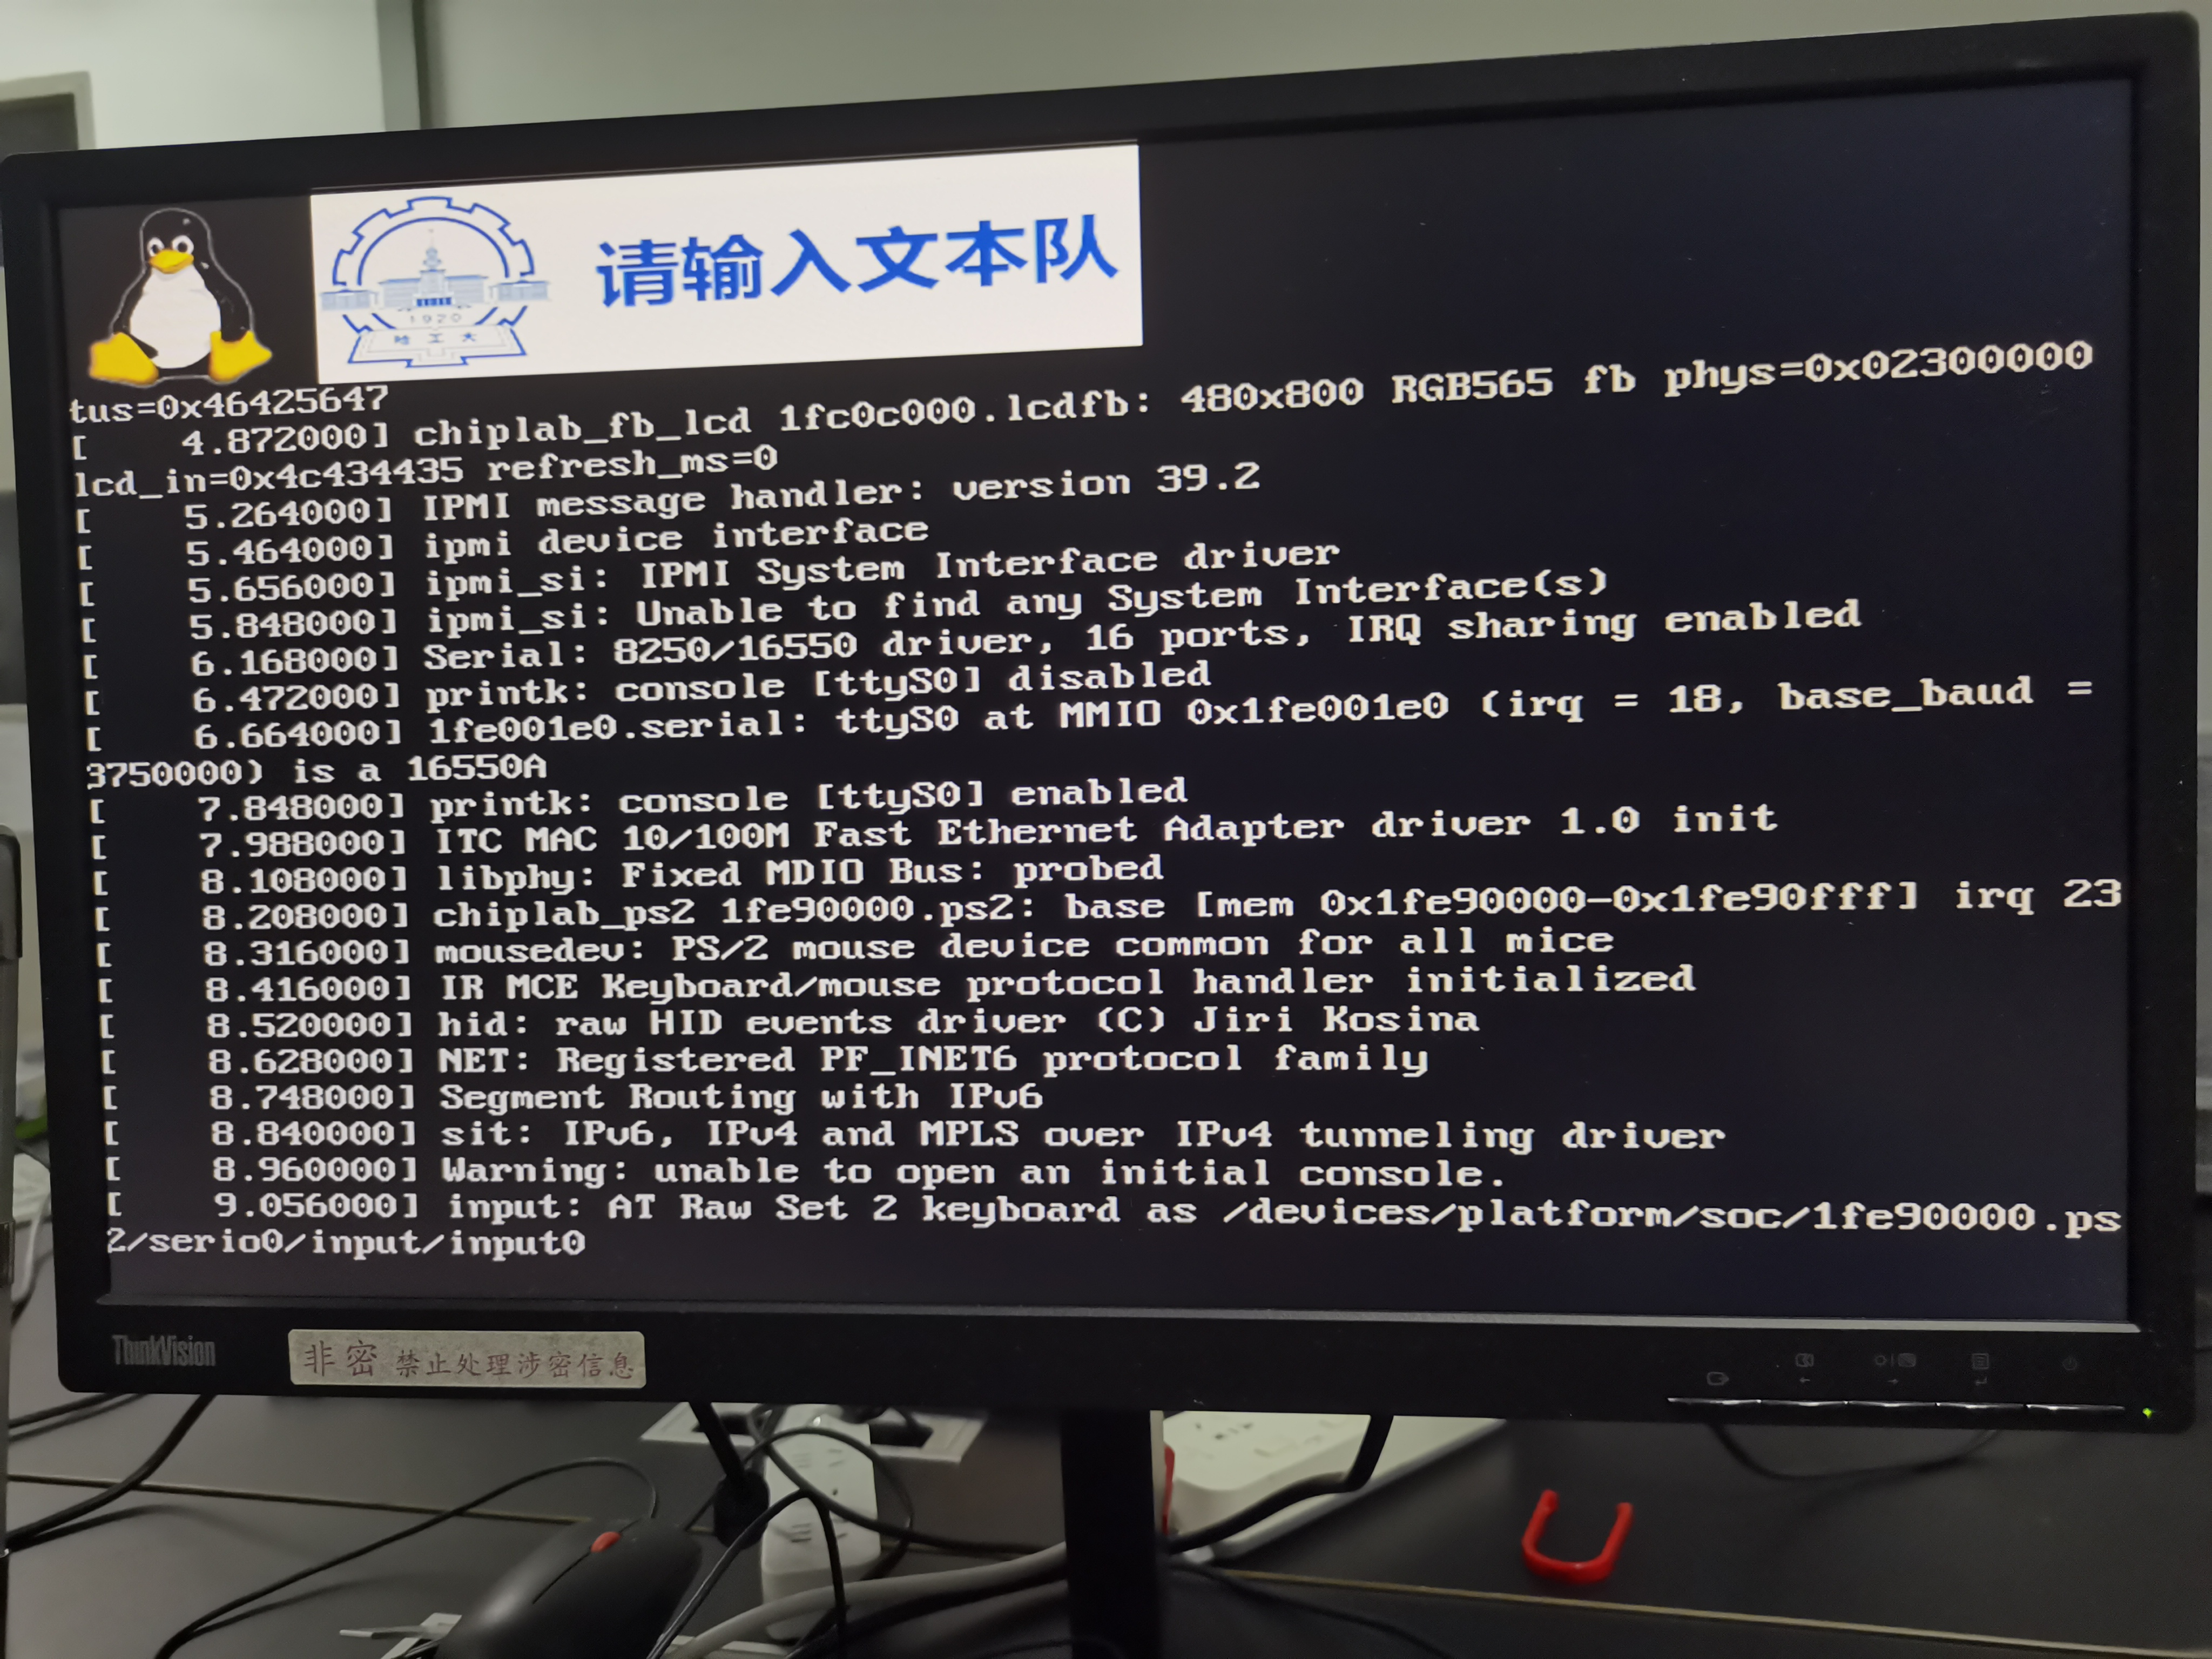
\includegraphics[width=0.95\textwidth]{figure/启动linux.jpg}
  \caption{linux启动}
  \label{fig:linux启动}
\end{figure}


\section{参考设计说明}

\begin{enumerate}
  \item \textbf{前端：满洋学长 / 404 NOT FOUND 队}\\
  我们重点参考了满洋学长的前端与分支预测相关设计（含 TAGE 等思路）
  %真的够吃好几届！
  我们结合本核负载对表项容量、历史长度与训练时机进行了调整，将分支预测率提高到98\%，这对多级流水的IPC有极大好处。\\
  源代码 URL：\url{https://github.com/HITSZ-NSCSCC22/mycpu}

  \item \textbf{*重点思路参考：Cache-HIT-100 队（朱炫翰、蔡源航、房效民、林亮宇）}\\
  %Cache-HIT-100团队给予了我们十分十分大的帮助！！！
  从前端来说，主要参考其解耦前端结构（BPU / FTB / FTQ / IFU / 预译码等）以及相关报告中的取指与预测流水划分，并完成了学长未完成的ubtb。
  
  %从前后端的解耦来说，点明了inst buffer的思路！！当时我们还不是学的很深入
  
  从后端来说，Cache-HIT-100团队已经具备了乱序的能力。只差唤醒。所以我们着重借鉴了ROB、RS等一系列设计，实现了本乱序核。\\
  
  %还有一点非常重要，大队长朱炫翰亲自教了我们要多看前人的设计，像mariver、满洋等！真想让朱学长再带我们冲一次。
  
  源代码 URL：\url{https://gitee.com/zxhzxhPhD/cache-hit-100-so-c}
  
  %不过，这个仓库是私有的，自己联系咱校的大队长朱炫翰�:)

  \item \textbf{后端、soc与linux：马家沟河队 Mariver（cpucore-mariver）}\\
  参考其乱序后端组织思路，包括重命名、分发、保留站/发射、ROB 写回与提交等阶段划分及执行通路设计。因为其为 mips 架构，所以我们迁移适配到 LA32R 与本核接口。
  
  同时他们的soc与linux也给了我们非常大的启发。包括中文输入法、GUI显示、LCD、3D 渲染等。\\
  %而且其ROB的队列设计太棒了！解决了PRF等的设计问题（解决就是我们不用PRF！）\\
  源代码 URL：\url{https://github.com/HIT-MaRiver-mips/cpucore-mariver}\\
  设计报告：\url{https://github.com/HIT-MaRiver-mips/report-mariver}

  \item \textbf{Uboot：JIT}\\
  JIT 团队将 uboot 的 tftp 内核加载速度提高到了 500KB/s ，参考他们的优化补丁，我们将其移植到了 uboot v2026 上\\
  源代码 URL：\url{https://github.com/nscscc24-jit-thu/u-boot-mainline}
  
  \item \textbf{openla500}\\
  主要参考流水线异常处理、地址翻译与 uncache 访问相关思路；乘除单元与 AXI 访问次序方面亦有借鉴。其中处理定时器中断的思路被我们用于解决功能测试第 49 个测试点。\\
  源代码 URL：\url{https://gitee.com/loongson-edu/open-la500}
  
  %\item \textbf{一个娱乐的游戏}\\
  %该游戏列在这里是因为这个给我们给予了许多欢笑与慰藉。没错，这个游戏是我们做的\verb|(*^▽^*)| 。
  %源代码 URL：\url{https://globalgamejam.org/games/2026/baimannailong-9}
  

\end{enumerate}

\section{参考文献}

\begin{enumerate}[leftmargin=2em,itemsep=4pt]
  \item 汪文祥, 邢金璋. CPU设计实战[M]. 北京: 机械工业出版社, 2021.
  \item 姚永斌. 超标量处理器设计[M]. 北京: 清华大学出版社, 2014.
\end{enumerate}


\end{document}
